%%%%%%%%%%%%%%%%%%%%%%%%%%%%%%%%%%%%%%%%%%%%%%%%%%%%%%%%%%%

\chapter{Modello del sistema - gruppo 1}
\label{ref:modSistemaGruppo1}

%%% Il gruppo 1 scriverà il suo modello del sistema. Esso dovrà includere: attori, casi d'uso (descrizione e tabella), scenari, diagrammi dei casi d'uso, diagrammi di sequenza, diagramma delle attività, screen mockups della funzionalità %%%

\section{Attori}
%%%%%%%%%%%%%%%%%% 8.1.1 Sync %%%%%%%%%%%%%%%%
\subsection{\textit{Sync}}
\paragraph{} 
\textit{Sync} rappresenta il sincronizzatore remoto, un web service esterno che si interfaccia con una serie di servizi tra cui \textit{Esse3}, ossia il portale dello studente che offre le funzionalità da replicare nell’applicazione, \textit{Aule Unimol}, e… È un’entità esterna al sistema che si vuole realizzare, pertanto  è classificata come attore.
\begin{center}
	
\includegraphics[height=3in]{imgs/gruppo1/Attore-Sync.pdf}
\end{center}

%%%%%%%%%%%%%%%%%% 8.1.2 Studente %%%%%%%%%%%%%%%%
\subsection{Studente}
\paragraph{} 
Studente regolarmente iscritto all’\textit{Università degli Studi Del Molise}, munito delle credenziali per accedere al portale dello studente \textit{Esse3}, il servizio esterno sul quale si basa l’applicazione. Lo studente utilizza l’applicazione per usufruire in maniera agevole dei servizi offerti dai portali dell’\textit{Università degli Studi del Molise} e monitorare la propria carriera universitaria.
\begin{center}
	
\includegraphics[height=3in]{imgs/gruppo1/Attore-Studente.pdf}
\end{center}

\section{Scenari}

%%%%%%%%%%%%%%%%%% 8.4.1 Visualizza corsi %%%%%%%%%%%%%%%%
\subsection{Visualizza corsi}
\paragraph{Visualizzazione avvenuta con successo.} 
Lo studente Giuseppe, iscritto al terzo anno della facoltà di Informatica, accede alla sezione \textit{Piano di studio} per visualizzare i corsi del piano di studio. Nello specifico, per ogni corso il sistema mostra il nome e, se superato, il voto e la data di verbalizzazione:

\begin{tabbing}
	%La prima righa non viene stampata, serve solo per la spaziatura
	\hspace{1cm}-----------------Esame--------------------------- \= --Voto--- \= --------Data------ \kill
	%Scrivere da qui
	\hspace{1cm} • Programmazione e laboratorio \> 25 \> 01/07/2018 \\
	\hspace{1cm} • Architettura degli elaboratori \> 28 \> 21/01/2018 \\
	\hspace{1cm} • Informatica giuridica \> 30 \> 07/06/2018 \\
	\hspace{1cm} • Matematica \> 24 \> 20/07/2018 \\
	\hspace{1cm} • Basi di dati e sistemi informativi \> 30 \> 15/07/2019 \\
	\hspace{1cm} • Calcolo numerico \> 18 \> 26/03/2019 \\
	\hspace{1cm} • Storia della matematica \> N/D \>\\
	\hspace{1cm} • Informatica territoriale \> N/D \>\\
	\hspace{1cm} • Statistica \> N/D \>\\
	\hspace{1cm} • Intelligenza artificiale \> N/D \>\\
	\hspace{1cm} • Programmazione mobile \> N/D \>\\
\end{tabbing}

%%%%%%%%%%%%%%%%%% 8.4.2 Ricerca corsi %%%%%%%%%%%%%%%%
\subsection{Ricerca corsi}
\paragraph{Ricerca avvenuta con successo.} 
Lo studente Giuseppe, iscritto al terzo anno della facoltà di Informatica, dopo aver visualizzato i corsi del piano di studio, inserisce la parola chiave \textbf{\textit{“Matematica”}}. Il sistema trova i corsi e mostra i risultati:

\begin{tabbing}
	%La prima righa non viene stampata, serve solo per la spaziatura
	\hspace{1cm}-----------------Esame--------------------------- \= --Voto--- \= --------Data------ \kill
	%Scrivere da qui
	\hspace{1cm} • Matematica \> 24 \> 20/07/2018 \\
	\hspace{1cm} • Storia della matematica \> N/D \>\\
\end{tabbing}

\paragraph{La ricerca non restituisce risultati.} 
Lo studente Giuseppe, iscritto al terzo anno della facoltà di Informatica, dopo aver visualizzato i corsi del piano di studio, inserisce la parola chiave \textbf{\textit{“Matemagica”}}. Il sistema non restituisce alcun riscontro e mostra allo studente il messaggio di errore “Nessun corso trovato”.

%%%%%%%%%%%%%%%%%% 8.4.3 Filtra corsi con memorizzazione   %%%%%%%%%%%%%%%%
\subsection{Filtra corsi con memorizzazione }
\paragraph{Filtra per anno.} 
Filtra per anno. Lo studente Giuseppe, iscritto al terzo anno della facoltà di Informatica, dopo aver visualizzato l’elenco dei corsi del piano di studio, applica il filtro per visualizzare gli esami del \textbf{secondo anno}. Il sistema mostra:

\begin{tabbing}
	%La prima righa non viene stampata, serve solo per la spaziatura
	\hspace{1cm}-----------------Esame--------------------------- \= --Voto--- \= --------Data------ \kill
	%Scrivere da qui
	\hspace{1cm} • Basi di dati e sistemi informativi \> 30 \> 15/07/2019 \\
	\hspace{1cm} • Calcolo numerico \> 18 \> 26/03/2019 \\
	\hspace{1cm} • Ingegneria del Software\> N/D \> \\
	\hspace{1cm} • Storia della matematica \> 30L \> 04/02/2019 \\
\end{tabbing}

\paragraph{Filtra esami superati.} 
Lo studente Giuseppe, iscritto al terzo anno della facoltà di Informatica, dopo aver visualizzato l’elenco dei corsi del piano di studio, applica il filtro per visualizzare gli\textbf{ esami superati}. Il sistema mostra:

\begin{tabbing}
	%La prima righa non viene stampata, serve solo per la spaziatura
	\hspace{1cm}-----------------Esame--------------------------- \= --Voto--- \= --------Data------ \kill
	%Scrivere da qui
	\hspace{1cm} • Programmazione e laboratorio \> 25 \> 01/07/2018 \\
	\hspace{1cm} • Architettura degli elaboratori \> 28 \> 21/01/2018 \\
	\hspace{1cm} • Informatica giuridica \> 30 \> 07/06/2018 \\
	\hspace{1cm} • Matematica \> 24 \> 20/07/2018 \\
	\hspace{1cm} • Basi di dati e sistemi informativi \> 30 \> 15/07/2019 \\
	\hspace{1cm} • Calcolo numerico \> 18 \> 26/03/2019 \\
\end{tabbing}

\paragraph{Memorizza filtro.}
 Lo studente Giuseppe, iscritto al terzo anno della facoltà di Informatica, dopo aver visualizzato l’elenco dei corsi del piano di studio ed aver applicato il filtro “esami da sostenere”, sceglie di memorizzarlo. Il sistema mantiene il filtro memorizzato anche in seguito alla chiusura del sistema. Alla successiva apertura dell’app, il sistema filtra di default i corsi per “esami da sostenere”.
 
\paragraph{Nessuna memorizzazione.}Lo studente Giuseppe, iscritto al terzo anno della facoltà di Informatica, dopo aver visualizzato l’elenco dei corsi del piano di studio ed aver applicato il filtro “esami da sostenere”, sceglie di non memorizzare le opzioni inserite. Il sistema applica il filtro selezionato fino alla chiusura del sistema. Alla successiva apertura dell'applicazione, il sistema mostra a Giuseppe tutti i corsi del piano di studio.

\paragraph{Il filtraggio non restituisce alcun risultato.}
Lo studente Giuseppe, iscritto al terzo anno della facoltà di Informatica, dopo aver visualizzato i corsi del piano di studio, applica il filtro “esami da sostenere” che non restituisce alcun risultato. Il sistema mostra allo studente il messaggio di errore “Nessun esame è stato trovato. Si prega di resettare le impostazioni precedentemente inserite!”


%%%%%%%%%%%%%%%%%% 8.4.4 Ordina corsi con memorizzazione%%%%%%%%%%%%%%%%
\subsection{Ordina corsi con memorizzazione}
\paragraph{Ordinamento alfabetico.}
Lo studente Giuseppe, iscritto al terzo anno della facoltà di Informatica, dopo aver visualizzato l’elenco dei corsi del piano di studio, applica l’ordinamento \textbf{alfabetico}. Il sistema mostra:

\begin{tabbing}
	%La prima righa non viene stampata, serve solo per la spaziatura
	\hspace{1cm}-----------------Esame--------------------------- \kill
	%Scrivere da qui
	\hspace{1cm} • Architettura degli elaboratori \\
	\hspace{1cm} • Basi di dati e sistemi informativi \\
	\hspace{1cm} • Calcolo numerico \\
	\hspace{1cm} • Informatica giuridica \\
	\hspace{1cm} • Matematica \\
	\hspace{1cm} • Programmazione e laboratorio \\
	\hspace{1cm} • Storia della matematica \\
\end{tabbing}

\paragraph{Ordinamento per anno.}
Lo studente Giuseppe, iscritto al terzo anno della facoltà di Informatica, dopo aver visualizzato l’elenco dei corsi del piano di studio, applica l’ordinamento per \textbf{anno}. Il sistema mostra:

\begin{tabbing}
	%La prima righa non viene stampata, serve solo per la spaziatura
	\hspace{1cm}-----------------Esame--------------------------- \= --anno---\kill
	%Scrivere da qui
	\hspace{1cm} • Programmazione e laboratorio \> Primo anno \\
	\hspace{1cm} • Matematica \> Primo anno \\
	\hspace{1cm} • Architettura degli elaboratori \> Primo anno \\
	\hspace{1cm} • Fisica \> Secondo anno \\
	\hspace{1cm} • Calcolo numerico \>Secondo anno \\
	\hspace{1cm} • Intelligenza artificiale	 \>Terzo anno \\
\end{tabbing}


\paragraph{Ordinamento per anno crescente.}
Lo studente Giuseppe, iscritto al terzo anno della facoltà di Informatica, dopo aver visualizzato l’elenco dei corsi del piano di studio, applica l’ordinamento per anno. Il sistema mostra:
	
\begin{tabbing}
	%La prima righa non viene stampata, serve solo per la spaziatura
	\hspace{1cm}-----------------Esame--------------------------- \= --anno---\kill
	%Scrivere da qui
	\hspace{1cm} • Programmazione e laboratorio \> Primo anno \\
	\hspace{1cm} • Matematica \> Primo anno \\
	\hspace{1cm} • Architettura degli elaboratori \> Primo anno \\
	\hspace{1cm} • Fisica \> Secondo anno \\
	\hspace{1cm} • Calcolo numerico \>Secondo anno \\
	\hspace{1cm} • Intelligenza artificiale	 \>Terzo anno \\	
\end{tabbing}

\paragraph{Ordinamento per anno decrescente.}
Lo studente Giuseppe iscritto al terzo anno della facoltà di Informatica, dopo aver visualizzato l'elenco dei corsi del piano di studio, applica l'ordinamento in modo crescente della configurazione in base all’anno. Il sistema mostra:

\begin{tabbing}
%La prima righa non viene stampata, serve solo per la spaziatura
\hspace{1cm}-----------------Esame--------------------------- \= --anno---\kill
%Scrivere da qui
\hspace{1cm} • Intelligenza artificiale	 \>Terzo anno \\
\hspace{1cm} • Fisica \> Secondo anno \\
\hspace{1cm} • Calcolo numerico \>Secondo anno \\	
\hspace{1cm} • Programmazione e laboratorio \> Primo anno \\
\hspace{1cm} • Matematica \> Primo anno \\
\hspace{1cm} • Architettura degli elaboratori \> Primo anno \\
\end{tabbing}

\paragraph{Ordinamento per CFU.}
Lo studente Giuseppe, iscritto al terzo anno della facoltà di Informatica, dopo aver visualizzato l’elenco dei corsi del piano di studio, applica l’ordinamento per \textbf{CFU}. Il sistema mostra:

\begin{tabbing}
	%La prima righa non viene stampata, serve solo per la spaziatura
	\hspace{1cm}-----------------Esame--------------------------- \= --CFU---\kill
	%Scrivere da qui
	\hspace{1cm} • Matematica \> 12 CFU \\
	\hspace{1cm} • Intelligenza artificiale	 \> 9 CFU \\
	\hspace{1cm} • Fisica \> 7 CFU \\
	\hspace{1cm} • Architettura degli elaboratori \> 6 CFU  \\
	\hspace{1cm} • Calcolo numerico \> 6 CFU \\	
	\hspace{1cm} • Inglese \> 6 CFU  \\	
	
\end{tabbing}

\paragraph{Ordinamento per CFU crescente.}
Lo studente Giuseppe iscritto al terzo anno della facoltà di Informatica, dopo aver visualizzato l'elenco dei corsi del piano di studio, applica l'ordinamento in modo crescente della configurazione in base ai  \textbf{CFU}. Il sistema mostra:

\begin{tabbing}
	%La prima righa non viene stampata, serve solo per la spaziatura
	\hspace{1cm}-----------------Esame--------------------------- \= --CFU---\kill
	%Scrivere da qui
	\hspace{1cm} • Inglese \> 6 CFU  \\	
	\hspace{1cm} • Calcolo numerico \> 6 CFU \\	
	\hspace{1cm} • Architettura degli elaboratori \> 6 CFU  \\
	\hspace{1cm} • Fisica \> 7 CFU \\
	\hspace{1cm} • Intelligenza artificiale	 \> 9 CFU \\
	\hspace{1cm} • Matematica \> 12 CFU \\
\end{tabbing}

\paragraph{Ordinamento per CFU decrescente.}
Lo studente Giuseppe iscritto al terzo anno della facoltà di Informatica, dopo aver visualizzato l'elenco dei corsi del piano di studio, applica l'ordinamento in modo decrescente della configurazione in base ai CFU. Il sistema mostra:

\begin{tabbing}
	%La prima righa non viene stampata, serve solo per la spaziatura
	\hspace{1cm}-----------------Esame--------------------------- \= --CFU---\kill
	%Scrivere da qui
	\hspace{1cm} • Matematica \> 12 CFU \\
	\hspace{1cm} • Intelligenza artificiale	 \> 9 CFU \\
	\hspace{1cm} • Fisica \> 7 CFU \\
	\hspace{1cm} • Architettura degli elaboratori \> 6 CFU  \\
	\hspace{1cm} • Calcolo numerico \> 6 CFU \\	
	\hspace{1cm} • Inglese \> 6 CFU  \\	
\end{tabbing}

\paragraph{Ordinamento per voto.}
 Lo studente Giuseppe, iscritto al terzo anno della facoltà di Informatica, dopo aver visualizzato l’elenco dei corsi del piano di studio, applica l’ordinamento per \textbf{voto}. Il sistema mostra:
 
 \begin{tabbing}
 	%La prima righa non viene stampata, serve solo per la spaziatura
 	\hspace{1cm}-----------------Esame--------------------------- \= --Voto--- \kill
 	%Scrivere da qui
   \hspace{1cm} • Storia della matematica \> 30L \\
   \hspace{1cm} • Informatica giuridica \> 30  \\
   \hspace{1cm} • Architettura degli elaboratori \> 28  \\
   \hspace{1cm} • Programmazione e laboratorio \> 25 \\
    \hspace{1cm} • Matematica \> 24  \\
     \hspace{1cm} • Calcolo numerico \> 18  \\
 \end{tabbing}
 
\paragraph{Ordinamento per voto crescente.}
Lo studente Giuseppe iscritto al terzo anno della facoltà di Informatica, dopo aver visualizzato l'elenco dei corsi del piano di studio, applica l'ordinamento in modo decrescente della configurazione in base ai voti. Il sistema mostra:

 \begin{tabbing}
	%La prima righa non viene stampata, serve solo per la spaziatura
	\hspace{1cm}-----------------Esame--------------------------- \= --Voto--- \kill
	%Scrivere da qui
	\hspace{1cm} • Calcolo numerico \> 18  \\
	\hspace{1cm} • Matematica \> 24  \\
	\hspace{1cm} • Programmazione e laboratorio \> 25 \\
	\hspace{1cm} • Architettura degli elaboratori \> 28  \\
	\hspace{1cm} • Informatica giuridica \> 30  \\
	\hspace{1cm} • Storia della matematica \> 30L \\
\end{tabbing}

\paragraph{Ordinamento per voto decrescente.}
Lo studente Giuseppe iscritto al terzo anno della facoltà di Informatica, dopo aver visualizzato l'elenco dei corsi del piano di studio, applica l'ordinamento in modo decrescente della configurazione in base ai voti. Il sistema mostra:

 \begin{tabbing}
	%La prima righa non viene stampata, serve solo per la spaziatura
	\hspace{1cm}-----------------Esame--------------------------- \= --Voto--- \kill
	%Scrivere da qui
	\hspace{1cm} • Storia della matematica \> 30L \\
	\hspace{1cm} • Informatica giuridica \> 30  \\
	\hspace{1cm} • Architettura degli elaboratori \> 28  \\
	\hspace{1cm} • Programmazione e laboratorio \> 25 \\
	\hspace{1cm} • Matematica \> 24  \\
	\hspace{1cm} • Calcolo numerico \> 18  \\
\end{tabbing}

\paragraph{Memorizza ordinamento.}
Lo studente Giuseppe, iscritto al terzo anno della facoltà di Informatica, dopo aver visualizzato l’elenco dei corsi del piano di studio ed aver applicato un ordinamento, sceglie di memorizzare le sue preferenze di ordinamento. Alla successiva apertura dell’applicazione, il sistema ordina i corsi sulla base dell'ultimo ordinamento memorizzato.

\paragraph{Nessuna memorizzazione.}
Lo studente Giuseppe, iscritto al terzo anno della facoltà di Informatica, dopo aver visualizzato l’elenco dei corsi del piano di studio ed aver applicato un ordinamento, sceglie di non memorizzare le sue preferenze di ordinamento. Il sistema mostra allo studente il messaggio “Le impostazioni non sono state salvate”. 

%%%%%%%%%%%%%%%%%% 8.4.5 Ordina corsi con memorizzazione%%%%%%%%%%%%%%%%
\subsection{Visualizza dettagli corso}
\paragraph{Visualizzazione dettagli di un corso superato.}
Lo studente Giuseppe, iscritto al terzo anno della facoltà di Informatica, sceglie di visualizzare i dettagli del corso superato di Informatica giuridica. Il sistema mostra allo studente i seguenti dettagli:

 \begin{tabbing}
	%La prima righa non viene stampata, serve solo per la spaziatura
	\hspace{1cm}-----------------info1--------------------------- \= --inforegistrata1--- \= --info2--\=--inofregistarta2 \kill
	%Scrivere da qui
	\hspace{1cm} • \textbf{Descrizione} Informatica giuridica \> \textbf{Docente} Troncarelli Barbara\\
	\hspace{1cm} • \textbf{Anno} 1 \> \textbf{CFU} 6   \\
	\hspace{1cm} • \textbf{Data esame} 19/06/2018 \> \textbf{Voto} 25 \\
\end{tabbing}

\paragraph{Visualizzazione dettagli di un corso non superato.}
Lo studente Giuseppe, iscritto al terzo anno della facoltà di Informatica, sceglie di visualizzare i dettagli del corso non superato di Ingegneria del software. Il sistema mostra allo studente i seguenti dettagli:

 \begin{tabbing}
	%La prima righa non viene stampata, serve solo per la spaziatura
	\hspace{1cm}-----------------info1--------------------------- \= --inforegistrata1--- \= --info2--\=--inofregistarta2 \kill
	%Scrivere da qui
	\hspace{1cm} • \textbf{Descrizione} Matematica \> \textbf{Docente} Giovanni  Capobianco\\
	\hspace{1cm} • \textbf{Anno} 1 \> \textbf{CFU} 12  \\
\end{tabbing}

%%%%%%%%%%%%%%%%%% 8.4.6  Visualizza appelli disponibili 
%%%%%%%%%%%%%%%%
\subsection{Visualizza appelli disponibili}
\paragraph{Visualizzazione avvenuta con successo.}
Lo studente Giuseppe, iscritto al terzo anno della facoltà di Informatica, sceglie di visualizzare gli appelli disponibili. Il sistema mostra:

 \begin{tabbing}
	%La prima righa non viene stampata, serve solo per la spaziatura
	\hspace{1cm}-----------------info1--------------------------- \= --inforegistrata1--- \= --info2--\=--inofregistarta2 \kill
	%Scrivere da qui
	\hspace{1cm} • \textbf{Descrizione} Basi di dati \> \textbf{Docente} Pareschi Remo
	  \\
	\hspace{1cm} •  \textbf{CFU} 12  \> \textbf{Data} 15/06/2019 \\
\end{tabbing}

\paragraph{Nessun appello disponibile.}
Lo studente Giuseppe, iscritto al terzo anno della facoltà di Informatica, sceglie di visualizzare gli appelli disponibili. Il sistema non restituisce alcun appello disponibile e mostra il messaggio di errore “Nessun appello disponibile”.

%%%%%%%%%%%%%%%%%% 8.4.7  Visualizza appelli prenotati
%%%%%%%%%%%%%%%%
\subsection{Visualizza appelli prenotati}
\paragraph{Visualizzazione avvenuta con successo.}
Lo studente Giuseppe, iscritto al terzo anno della facoltà di Informatica, visualizza gli appelli prenotati. Il sistema mostra i dati relativi agli appelli prenotati: 

 \begin{tabbing}
	%La prima righa non viene stampata, serve solo per la spaziatura
	\hspace{1cm}-----------------esame---------------------------\=--Data---\= --tipologia--\kill
	%Scrivere da qui
	\hspace{1cm} • Fisica \> 01/03/2019 \> Orale \\
\end{tabbing}

\paragraph{Nessun appello prenotato.}
Lo studente Giuseppe, iscritto al terzo anno della facoltà di Informatica, visualizza gli appelli prenotati. Il sistema non restituisce alcun appello prenotato e mostra il messaggio di errore “Nessun appello prenotato”. 

%%%%%%%%%%%%%%%%%% 8.4.8  Visualizza appelli prenotati
%%%%%%%%%%%%%%%%

\subsection{Ricerca appelli disponibili}
\paragraph{Ricerca avvenuta con successo.}
Lo studente Giuseppe, iscritto al terzo anno della facoltà di Informatica, dopo aver visualizzato gli appelli disponibili, inserisce la parola chiave \textbf{\textit{“Matematica”}}. Il sistema trova gli appelli disponibili e mostra i risultati:

\begin{tabbing}
	%La prima righa non viene stampata, serve solo per la spaziatura
	\hspace{1cm}-----------------esame---------------------------\=--Data---\kill
	%Scrivere da qui
	\hspace{1cm} • Matematica  \> 16/02/2019  \\
	\hspace{1cm} • Storia della Matematica \> 18/01/2019 \\
\end{tabbing}

\paragraph{La ricerca non restituisce risultati.}
Lo studente Giuseppe, iscritto al terzo anno della facoltà di Informatica, dopo aver visualizzato gli appelli disponibili, inserisce la parola chiave \textbf{\textit{“Matemagica”}}. Il sistema non restituisce alcun riscontro e mostra allo studente il messaggio di errore “Nessun appello trovato”.

%%%%%%%%%%%%%%%%%% 8.4.9  Filtra appelli disponibili con memorizzazione
%%%%%%%%%%%%%%%%

\subsection{Filtra appelli disponibili con memorizzazione}
\paragraph{Filtra per tipologia d’esame: scritto.}
Lo studente Giuseppe, iscritto al terzo anno della facoltà di Informatica, dopo aver visualizzato l’elenco degli appelli disponibili, sceglie di filtrare gli esami per tipologia \textbf{“scritto”}. Il sistema mostra:  

 \begin{tabbing}
	%La prima righa non viene stampata, serve solo per la spaziatura
	\hspace{1cm}-----------------esame---------------------------\=--Data---\= --tipologia--\kill
	%Scrivere da qui
	\hspace{1cm} • Calcolo numerico  \> 26/03/2019 \> Scritto \\
	\hspace{1cm} • Ingegneria del Software \> 01/04/2019 \> Scritto-Orale  \\
\end{tabbing}

\paragraph{Filtra per tipologia d’esame: orale.}
Lo studente Giuseppe, iscritto al terzo anno della facoltà di Informatica, dopo aver visualizzato l’elenco degli appelli disponibili, sceglie di filtrare gli appelli per tipologia di esame \textbf{“orale”}. Il sistema mostra:

 \begin{tabbing}
	%La prima righa non viene stampata, serve solo per la spaziatura
	\hspace{1cm}-----------------esame---------------------------\=--Data---\= --tipologia--\kill
	%Scrivere da qui
	\hspace{1cm} • Informatica giuridica  \> 10/04/2019\> Orale \\
	\hspace{1cm} • Matematica\> 18/04/2019 \> Orale-Scritto  \\
\end{tabbing}

\paragraph{Filtra per anno.}
Lo studente Giuseppe, iscritto al terzo anno della facoltà di Informatica, dopo aver visualizzato l’elenco degli appelli disponibili, sceglie di filtrare in base all'anno in cui è previsto il corso e sceglie di filtrare gli appelli per visualizzare solo quelli afferenti al \textbf{secondo anno}. Il sistema mostra:

\begin{tabbing}
	%La prima righa non viene stampata, serve solo per la spaziatura
	\hspace{1cm}-----------------Esame--------------------------- \= --Voto--- \= --------Data------ \kill
	%Scrivere da qui
	\hspace{1cm} • Basi di dati e sistemi informativi \> 30 \> 15/07/2019 \\
	\hspace{1cm} • Calcolo numerico \> 18 \> 26/06/2019 \\
	\hspace{1cm} • Fisica \> 28 \> 29/06/2019 \\
	\hspace{1cm} • Ingegneria del Software \> N/D \> 7/06/2019  \\
\end{tabbing}

\paragraph{Memorizza filtro.}
Lo studente Giuseppe, iscritto al terzo anno della facoltà di Informatica, dopo aver visualizzato l’elenco degli appelli disponibili ed aver applicato il filtro “anno”, sceglie di memorizzarlo. Il sistema mantiene il filtro memorizzato anche in seguito alla chiusura del sistema . Alla successiva apertura dell’app, il sistema filtra di default gli appelli per “anno”.

\paragraph{Nessuna memorizzzazione.}
Lo studente Giuseppe, iscritto al terzo anno della facoltà di Informatica, dopo aver visualizzato l’elenco degli appelli disponibili ed aver applicato un filtro, sceglie di non memorizzare le opzioni inserite. Alla successiva apertura dell'applicazione, il sistema mostra a Giuseppe tutti gli appelli disponibili.

\paragraph{Il filtraggio non restituisce alcun risultato.}
 Lo studente Giuseppe, iscritto al terzo anno della facoltà di Informatica, dopo aver scelto di filtrare gli appelli disponibili in base al parametro selezionato, non riceve risultati dal sistema. Il sistema mostra il messaggio “Nessun appello è stato trovato. Si prega di resettare le impostazioni precedentemente inserite!”
 
 %%%%%%%%%%%%%%%%%% 8.4.10  Ordina appelli disponibili con memorizzazione
 %%%%%%%%%%%%%%%%
 
\subsection{Ordina appelli disponibili con memorizzazione}
\paragraph{Ordinamento alfabetico.}
Lo studente Giuseppe, iscritto al terzo anno della facoltà di Informatica, decide di ordinare la lista degli appelli disponibili usando il criterio di ordinamento alfabetico degli appelli. Ad ordinamento effettuato, il sistema mostra i seguenti esami:

\begin{tabbing}
	%La prima righa non viene stampata, serve solo per la spaziatura
	\hspace{1cm}-----------------Esame--------------------------- \= --Data--- \= --------Docente------ \kill
	%Scrivere da qui
	\hspace{1cm} • Algoritmi e Strutture Dati \> 07/04/2019 \> G. Parlato \\
	\hspace{1cm} • Calcolo numerico \> 05/04/2019  \> G. Capobianco \\
	\hspace{1cm} • Fisica \> 06/04/2019 \> G. M. Piacentino  \\
	\hspace{1cm} • Ingegneria del Software \> 04/04/2019   \> F. Fasano \\
\end{tabbing}

\paragraph{Ordinamento per data.}
 Lo studente Giuseppe, iscritto al terzo anno della facoltà di Informatica, decide di ordinare la lista degli appelli disponibili usando il criterio di ordinamento per data. Ad ordinamento effettuato, il sistema mostra i seguenti esami:
 
\begin{tabbing}
	%La prima righa non viene stampata, serve solo per la spaziatura
	\hspace{1cm}-----------------Esame--------------------------- \= --Data--- \= --------Docente------ \kill
	%Scrivere da qui
	\hspace{1cm} • Ingegneria del Software \> 04/04/2019   \> F. Fasano \\
	\hspace{1cm} • Calcolo numerico \> 05/04/2019  \> G. Capobianco \\
	\hspace{1cm} • Fisica \> 06/04/2019 \> G. M. Piacentino  \\
	\hspace{1cm} • Algoritmi e Strutture Dati \> 07/04/2019 \> G. Parlato \\
\end{tabbing} 

\paragraph{Ordinamento per docente.}
Lo studente Giuseppe, iscritto al terzo anno della facoltà di Informatica, decide di ordinare la lista degli appelli disponibili usando il criterio di ordinamento per cognome del docente. Ad ordinamento effettuato, il sistema mostra i seguenti esami:

\begin{tabbing}
	%La prima righa non viene stampata, serve solo per la spaziatura
	\hspace{1cm}-----------------Esame--------------------------- \= --Data--- \= --------Docente------ \kill
	%Scrivere da qui
	\hspace{1cm} • Calcolo numerico \> 05/04/2019  \> G. Capobianco \\
	\hspace{1cm} • Ingegneria del Software \> 04/04/2019   \> F. Fasano \\
	\hspace{1cm} • Algoritmi e Strutture Dati \> 07/04/2019 \> G. Parlato \\	
	\hspace{1cm} • Fisica \> 06/04/2019 \> G. M. Piacentino  \\
\end{tabbing} 

\paragraph{Memorizza ordinamento.}
Lo studente Giuseppe, iscritto al terzo anno della facoltà di Informatica, dopo aver visualizzato l’elenco degli appelli disponibili ed aver applicato un ordinamento per data, sceglie di memorizzare le sue preferenze di ordinamento. Alla successiva apertura dell’applicazione, il sistema ordina gli appelli disponibili sulla base dell'ultimo ordinamento memorizzato.

\paragraph{Nessuna memorizzazione.}
Lo studente Giuseppe, iscritto al terzo anno della facoltà di Informatica, dopo aver visualizzato l’elenco degli appelli disponibili ed aver applicato un ordinamento, sceglie di non memorizzare le sue preferenze di ordinamento. Il sistema mostra allo studente il messaggio “Le impostazioni non sono state salvate”.

 %%%%%%%%%%%%%%%%%% 8.4.11  Prenota appello %%%%%%%%%%%%%%%%

\subsection{Prenota appello}
\paragraph{Prenotazione effettuata con successo.}
Lo studente Giuseppe, iscritto al terzo anno della facoltà di Informatica, dopo aver visualizzato la lista degli appelli disponibili, sceglie di prenotare l’appello di \textit{Fisica} e lo seleziona dalla lista. Il sistema effettua la prenotazione all’appello e mostra il messaggio “La prenotazione è stata confermata”.

\paragraph{Prenotazione fallita.}
Lo studente Giuseppe, iscritto al terzo anno della facoltà di Informatica, dopo aver visualizzato la lista degli appelli disponibili, sceglie di prenotare l’appello di \textit{Fisica} e lo seleziona dalla lista. Il sistema prova ad effettuare la prenotazione ma l’operazione non ha successo, per cui mostra il messaggio di errore “Impossibile effettuare la prenotazione”.

 %%%%%%%%%%%%%%%%%% 8.4.12 Cancella prenotazione %%%%%%%%%%%%%%%%

\subsection{Cancella prenotazione}
\paragraph{Cancellazione della prenotazione effettuata con successo.}
Lo studente Giuseppe, iscritto al terzo anno della facoltà di Informatica, dopo aver visualizzato la lista degli appelli prenotati, sceglie di cancellare la prenotazione all’appello di \textit{Ingegneria del software} e lo seleziona dalla lista. Il sistema annulla la prenotazione all’appello e mostra il messaggio “La prenotazione è stata annullata con successo”.

\paragraph{Cancellazione della prenotazione effettuata con successo.}
Lo studente Giuseppe, iscritto al terzo anno della facoltà di Informatica, dopo aver visualizzato la lista degli appelli prenotati, sceglie di cancellare la prenotazione all’appello di \textit{Ingegneria del software} previsto e lo seleziona dalla lista. Il sistema prova a cancellare la prenotazione, ma l’operazione non ha successo, per cui il sistema mostra il messaggio di errore “Impossibile annullare la prenotazione”.

%%%%%%%%%%%%%%%%%% 8.4.13  Visualizza elenco file %%%%%%%%%%%%%%%%
\subsection{Visualizza elenco file}
\paragraph{Visualizzazione elenco file avvenuta con successo.}
Lo studente Giuseppe, iscritto al terzo anno della facoltà di Informatica, dopo aver visualizzato la lista dei corsi, seleziona il corso di \textit{Informatica giuridica} e chiede di visualizzarne il materiale didattico. Il sistema mostra allo studente i seguenti file: 

\begin{tabbing}
	%La prima righa non viene stampata, serve solo per la spaziatura
	\hspace{1cm}-----------------File---------------------------\kill
	%Scrivere da qui
	\hspace{1cm} • Interventi in aula.pdf  \\
	\hspace{1cm} • Link utili.pdf  \\
	\hspace{1cm} • Programma di dettaglio.pdf  \\	
	\hspace{1cm} • Slides.pdf  \\
\end{tabbing} 

\paragraph{Nessun file.}
 Lo studente Giuseppe, iscritto al terzo anno della facoltà di Informatica, dopo aver visualizzato la lista dei corsi, seleziona il corso di Evoluzione del calcolo automatico  e chiede di visualizzarne il materiale didattico. Il sistema cerca i file di \textit{Evoluzione del calcolo automatico}, ma non trova nessun file, quindi mostra il messaggio “Nessun file disponibile”
 
%%%%%%%%%%%%%%%%%% 8.4.14  Ricerca file %%%%%%%%%%%%%%%%
\subsection{Ricerca file}
\paragraph{Ricerca avvenuta con successo.}
Lo studente Giuseppe, iscritto al terzo anno della  facoltà di Informatica, dopo aver visualizzato l’elenco del materiale didattico del corso di Informatica giuridica, inserisce la parola chiave \textbf{“Slides”}. Il sistema trova il file e mostra i risultati:   

\begin{tabbing}
	%La prima righa non viene stampata, serve solo per la spaziatura
	\hspace{1cm}-----------------File---------------------------\kill
	%Scrivere da qui
	\hspace{1cm} • Slides.pdf  \\
\end{tabbing} 

\paragraph{La ricerca non restituisce risultati.}
Lo studente Giuseppe, iscritto al terzo anno della facoltà di Informatica, dopo aver visualizzato l’elenco del materiale didattico del corso di Informatica giuridica, inserisce la parola chiave “Sliders”. Il sistema non restituisce alcun riscontro e mostra allo studente il messaggio di errore “Nessun file trovato”.

%%%%%%%%%%%%%%%%%% 8.4.15  Visualizza dettagli file %%%%%%%%%%%%%%%%
\subsection{ Visualizza dettagli file}
\paragraph{Visualizzazione dettagli file avvenuta con successo.}
Lo studente Giuseppe, iscritto al terzo anno della facoltà di Informatica, dopo aver visualizzato l’elenco del materiale didattico del corso di \textit{Informatica giuridica}, seleziona il file \textit{Slides.pdf}. Il sistema elabora la richiesta e mostra allo studente i seguenti dettagli relativi al file selezionato:

\begin{tabbing}
	%La prima righa non viene stampata, serve solo per la spaziatura
	\hspace{1cm}-----------------Info---------------------------\= infoRegistrate\kill
	%Scrivere da qui
	\hspace{1cm} • \textbf{Nome file} \> Slides.pdf  \\
	\hspace{1cm} • \textbf{Docente/i} \> Troncarelli Barbara  \\
	\hspace{1cm} • \textbf{Data} \> 10/02/2019  \\
	\hspace{1cm} • \textbf{Note} \> In allegato il materiale didattico presentato nelle lezioni dell'anno accademico 2017-18  \\
\end{tabbing} 

%%%%%%%%%%%%%%%%%% 8.4.16  Apri file  %%%%%%%%%%%%%%%%
\subsection{ Apri file}
\paragraph{Apertura del file avvenuta con successo.}
Lo studente Giuseppe, iscritto al terzo anno della facoltà di Informatica, dopo aver visualizzato i dettagli relativi al file \textit{Slides.pdf}, sceglie di aprirlo dalla schermata che ne mostra i dettagli. Il sistema cerca il file all'interno dello \textit{storage}, mostrando il suo contenuto allo studente.

\paragraph{File non presente nello \textbf{storage}.}
Lo studente Giuseppe, iscritto al terzo anno della facoltà di Informatica, dopo aver visualizzato i dettagli relativi al file \textit{Slides.pdf}, sceglie di aprirlo dalla schermata che ne mostra i dettagli. Il sistema cerca il file all'interno dello storage e, non trovandolo, mostra il messaggio “Il file non è presente sul dispositivo. Vuoi scaricarlo ora?”. Giuseppe conferma, il sistema scarica il file e successivamente lo apre.

%%%%%%%%%%%%%%%%%% 8.4.17  Rimuovi file  %%%%%%%%%%%%%%%%
\subsection{Rimuovi file}
\paragraph{Rimozione del file avvenuta con successo.}
Lo studente Giuseppe, iscritto al terzo anno della facoltà di Informatica, dopo aver visualizzato i dettagli relativi al file \textit{Slides.pdf}, chiede al sistema di rimuoverlo. Il sistema cerca il file all'interno dello \textit{storage} e lo rimuove, successivamente mostra il messaggio “File rimosso con successo”.
	
\paragraph{File non presente nello \textbf{storage}.}
Lo studente Giuseppe, iscritto al terzo anno della facoltà di Informatica, dopo aver visualizzato i dettagli relativi al file \textit{Slides.pdf}, chiede al sistema di rimuoverlo. Il sistema cerca il file all'interno delloe e, non trovandolo, mostra il messaggio di errore “Impossibile rimuovere file”.



\newpage


\begin{table} [tb]
	\section{Casi d'uso}
	\subsection{Visualizza corsi}
	Questo caso d’uso consentirà allo studente di visualizzare i corsi afferenti al suo piano di studio e includerà il caso d’uso \textit{getJson} passandogli l’ID del servizio per ottenere la lista di tutti i corsi. Quest’ultimo elaborerà la richiesta e restituirà i dati relativi ai corsi del piano di studio, dopodiché il sistema li mostrerà allo studente. Segue il diagramma dei casi d'uso corrispondente a questo caso d'uso: referenza
	 
	%\normalsize % Dimensione testo normale
	\small % Dimensione testo piccola
	%\footnotesize % Dimensione testo piccolissima
	%\scriptsize % Dimensione del testo ulteriormente più piccola
	%\caption{} % Didascalia tabella
	%\label{} % Etichetta per riferimenti incrociati
	\begin{tabular}{| p{\useCaseLeft} | p{\useCaseNum} | p{\useCaseTwoCol} | p{\useCaseTwoCol} |}
		\hline
		\textbf{Nome caso d'uso} & \multicolumn{3}{p{\useCaseMulticol} |}{\textbf{Visualizza corsi}} \\
		\hline
		\textbf{Attori partecipanti} & \multicolumn{3}{p{\useCaseMulticol} |}{Iniziato da \textit{Studente}.} \\
		\hline
		\textbf{Condizioni d'ingresso} & \multicolumn{3}{p{\useCaseMulticol} |}{Lo studente si trova nella sezione \textit{Piano di studio.}} \\
		\hline
		\textbf{Flusso degli eventi} & \textbf{\#} & \textbf{Studente} & \textbf{Sistema} \\
		\hline
		\textbf{} & \textbf{1} & Visualizza l’ultima copia dei corsi salvata nello \textit{storage.} & \textbf{} \\
		\hline
		\textbf{} & \textbf{2} & \textbf{} & Include il caso d’uso \textit{getJson} passandogli l’ID del servizio per la visualizzazione dei corsi. \\
		\hline
		\textbf{} & \textbf{3} & \textbf{} & Ottiene i corsi del piano di studio aggiornati e li mostra a video. \\
		\hline
		\textbf{Eccezioni} & \multicolumn{3}{p{\useCaseMulticol} |}{} \\
		\hline
		\textbf{Condizioni d'uscita} & \multicolumn{3}{p{\useCaseMulticol} |}{Lo studente visualizza i corsi aggiornati del piano di studio.} \\
		\hline
	\end{tabular}
\end{table}
\newpage


\begin{table}[tb]
	\subsection{Ricerca corsi}
	Questo caso d’uso consentirà allo studente di ricercare i corsi utilizzando delle parole chiave. Il sistema, dopo aver eseguito la ricerca, mostrerà i corsi trovati. Segue il diagramma dei casi d'uso corrispondente a questo caso d'uso: referenza
	%\normalsize % Dimensione testo normale
	\small % Dimensione testo piccola
	%\footnotesize % Dimensione testo piccolissima
	%\scriptsize % Dimensione del testo ulteriormente più piccola
	%\caption{} % Didascalia tabella
	%\label{} % Etichetta per riferimenti incrociati
	\begin{tabular}{| p{\useCaseLeft} | p{\useCaseNum} | p{\useCaseTwoCol} | p{\useCaseTwoCol} |}
		\hline
		\textbf{Nome caso d'uso} & \multicolumn{3}{p{\useCaseMulticol} |}{\textbf{Ricerca corsi}} \\
		\hline
		\textbf{Attori partecipanti} & \multicolumn{3}{p{\useCaseMulticol} |}{Iniziato da \textit{Studente}.} \\
		\hline
		\textbf{Condizioni d'ingresso} & \multicolumn{3}{p{\useCaseMulticol} |}{Lo studente visualizza i corsi del piano di studio.} \\
		\hline
		\textbf{Flusso degli eventi} & \textbf{\#} & \textbf{Studente} & \textbf{Sistema} \\
		\hline
		\textbf{} & \textbf{1} & Inserisce delle parole chiave. & \textbf{} \\
		\hline
		\textbf{} & \textbf{2} & \textbf{} & Esegue la ricerca. \\
		\hline
		\textbf{} & \textbf{3} & \textbf{} & Mostra i corsi che corrispondono alle parole chiave. \\
		\hline
		\textbf{Eccezioni} & \multicolumn{3}{p{\useCaseMulticol} |}{\textbf{2.1} Nessun risultato} \\
		\hline
		\textbf{Condizioni d'uscita} & \multicolumn{3}{p{\useCaseMulticol} |}{Lo studente visualizza i corsi trovati.} \\
		\hline
	\end{tabular}
\end{table}
\newpage


\begin{table}[tb]
	\subsection{Filtra corsi con memorizzazione}
	Questo caso d’uso consentirà allo studente di filtrare i corsi in base ad uno o più filtri. Il sistema, dopo aver filtrato l’elenco, mostrerà la lista di corsi filtrati. Lo studente avrà la possibilità di memorizzare i filtri nello \textit{storage} per visualizzare i dati filtrati ad ogni nuovo accesso alla sezione. Segue il diagramma dei casi d'uso corrispondente a questo caso d'uso: referenza
	%\normalsize % Dimensione testo normale
	\small % Dimensione testo piccola
	%\footnotesize % Dimensione testo piccolissima
	%\scriptsize % Dimensione del testo ulteriormente più piccola
	%\caption{} % Didascalia tabella
	%\label{} % Etichetta per riferimenti incrociati
	\begin{tabular}{| p{\useCaseLeft} | p{\useCaseNum} | p{\useCaseTwoCol} | p{\useCaseTwoCol} |}
		\hline
		\textbf{Nome caso d'uso} & \multicolumn{3}{p{\useCaseMulticol} |}{\textbf{Filtra corsi con memorizzazione}} \\
		\hline
		\textbf{Attori partecipanti} & \multicolumn{3}{p{\useCaseMulticol} |}{Iniziato da \textit{Studente}.} \\
		\hline
		\textbf{Condizioni d'ingresso} & \multicolumn{3}{p{\useCaseMulticol} |}{Lo studente visualizza i corsi del piano di studio.} \\
		\hline
		\textbf{Flusso degli eventi} & \textbf{\#} & \textbf{Studente} & \textbf{Sistema} \\
		\hline
		\textbf{} & \textbf{1} & Inserisce uno o più filtri. & \textbf{} \\
		\hline
		\textbf{} & \textbf{2} & \textbf{} & Filtra l’elenco dei corsi. \\
		\hline
		\textbf{} & \textbf{3} & \textbf{} & Mostra i corsi filtrati. \\
		\hline
		\textbf{} & \textbf{4} & Sceglie di salvare i filtri. & \textbf{} \\
		\hline
		\textbf{} & \textbf{5} &  \textbf{} & Memorizza i filtri nello \textit{storage}.\\
		\hline
		\textbf{Eccezioni} & \multicolumn{3}{p{\useCaseMulticol} |}{\textbf{4.1} Nessuna memorizzazione.\newline \textbf{5.1} Nessun risultato.} \\
		\hline
		\textbf{Condizioni d'uscita} & \multicolumn{3}{p{\useCaseMulticol} |}{Lo studente visualizza i corsi filtrati ed eventualmente salva i filtri. } \\
		\hline
	\end{tabular}
\end{table}
\newpage


\begin{table}[tb]
	\subsection{Ordina corsi con memorizzazione}
	Questo caso d’uso consentirà allo studente di ordinare i corsi in base ad un criterio di ordinamento. Il sistema, dopo aver ordinato l’elenco, mostrerà la lista di corsi ordinati. Lo studente avrà la possibilità di memorizzare il criterio di ordinamento nello \textit{storage}. Segue il diagramma dei casi d'uso corrispondente a questo caso d'uso: referenza
	%\normalsize % Dimensione testo normale
	\small % Dimensione testo piccola
	%\footnotesize % Dimensione testo piccolissima
	%\scriptsize % Dimensione del testo ulteriormente più piccola
	%\caption{} % Didascalia tabella
	%\label{} % Etichetta per riferimenti incrociati
	\begin{tabular}{| p{\useCaseLeft} | p{\useCaseNum} | p{\useCaseTwoCol} | p{\useCaseTwoCol} |}
		\hline
		\textbf{Nome caso d'uso} & \multicolumn{3}{p{\useCaseMulticol} |}{\textbf{Ordina corsi con memorizzazione}} \\
		\hline
		\textbf{Attori partecipanti} & \multicolumn{3}{p{\useCaseMulticol} |}{Iniziato da \textit{Studente}.} \\
		\hline
		\textbf{Condizioni d'ingresso} & \multicolumn{3}{p{\useCaseMulticol} |}{Lo studente visualizza i corsi del piano di studio.} \\
		\hline
		\textbf{Flusso degli eventi} & \textbf{\#} & \textbf{Studente} & \textbf{Sistema} \\
		\hline
		\textbf{} & \textbf{1} & Inserisce un criterio di ordinamento. & \textbf{} \\
		\hline
		\textbf{} & \textbf{2} & \textbf{} & Ordina l’elenco dei corsi. \\
		\hline
		\textbf{} & \textbf{3} & \textbf{} & Mostra i corsi ordinati. \\
		\hline
		\textbf{} & \textbf{4} & Sceglie di salvare il criterio di ordinamento selezionato. & \textbf{} \\
		\hline
		\textbf{} & \textbf{5} &  \textbf{} & Memorizza nello \textit{storage} il criterio di ordinamento.\\
		\hline
		\textbf{Eccezioni} & \multicolumn{3}{p{\useCaseMulticol} |}{\textbf{3.1} Nessuna memorizzazione.} \\
		\hline
		\textbf{Condizioni d'uscita} & \multicolumn{3}{p{\useCaseMulticol} |}{Lo studente visualizza i corsi ordinati ed eventualmente salva il criterio di ordinamento.} \\
		\hline
	\end{tabular}
\end{table}
\newpage


\begin{table}[tb]
	\subsection{Visualizza dettagli corso }
	Questo caso d’uso consentirà allo studente di visualizzare i dettagli di un corso e includerà il caso d’uso \textit{getJson} passandogli l’ID del servizio per ottenere i dettagli del corso selezionato. Quest’ultimo elaborerà la richiesta e restituirà i dati relativi al corso selezionato. Il sistema mostrerà allo studente i dettagli del corso selezionato. Segue il diagramma dei casi d'uso corrispondente a questo caso d'uso: referenza
	%\normalsize % Dimensione testo normale
	\small % Dimensione testo piccola
	%\footnotesize % Dimensione testo piccolissima
	%\scriptsize % Dimensione del testo ulteriormente più piccola
	%\caption{} % Didascalia tabella
	%\label{} % Etichetta per riferimenti incrociati
	\begin{tabular}{| p{\useCaseLeft} | p{\useCaseNum} | p{\useCaseTwoCol} | p{\useCaseTwoCol} |}
		\hline
		\textbf{Nome caso d'uso} & \multicolumn{3}{p{\useCaseMulticol} |}{\textbf{Visualizza dettagli corso}} \\
		\hline
		\textbf{Attori partecipanti} & \multicolumn{3}{p{\useCaseMulticol} |}{Iniziato da \textit{Studente}.} \\
		\hline
		\textbf{Condizioni d'ingresso} & \multicolumn{3}{p{\useCaseMulticol} |}{Lo studente visualizza i corsi del piano di studio.} \\
		\hline
		\textbf{Flusso degli eventi} & \textbf{\#} & \textbf{Studente} & \textbf{Sistema} \\
		\hline
		\textbf{} & \textbf{1} & Seleziona un corso di cui visualizzare i dettagli. & \textbf{} \\
		\hline
		\textbf{} & \textbf{2} & \textbf{} & Include il caso d’uso \textit{getJson} passandogli l’ID del servizio. \\
		\hline
		\textbf{} & \textbf{3} & \textbf{} & Mostra i dettagli relativi al corso selezionato. \\
		\hline
		\textbf{Eccezioni} & \multicolumn{3}{p{\useCaseMulticol} |}{} \\
		\hline
		\textbf{Condizioni d'uscita} & \multicolumn{3}{p{\useCaseMulticol} |}{Lo studente visualizza i dettagli relativi al corso selezionato.} \\
		\hline
	\end{tabular}
\end{table}
\newpage


\begin{table}[tb]
	\subsection{Visualizza appelli disponibili}
	Questo caso d’uso consentirà allo studente di visualizzare gli appelli disponibili afferenti ai corsi del suo piano di studio e includerà il caso d’uso \textit{getJson} passandogli l’ID del servizio per ottenere una lista contenente tutti gli appelli disponibili. Quest’ultimo elaborerà la richiesta e restituirà i dati relativi agli appelli disponibili. Il sistema mostrerà allo studente gli appelli disponibili. Segue il diagramma dei casi d'uso corrispondente a questo caso d'uso: referenza
	%\normalsize % Dimensione testo normale
	\small % Dimensione testo piccola
	%\footnotesize % Dimensione testo piccolissima
	%\scriptsize % Dimensione del testo ulteriormente più piccola
	%\caption{} % Didascalia tabella
	%\label{} % Etichetta per riferimenti incrociati
	\begin{tabular}{| p{\useCaseLeft} | p{\useCaseNum} | p{\useCaseTwoCol} | p{\useCaseTwoCol} |}
		\hline
		\textbf{Nome caso d'uso} & \multicolumn{3}{p{\useCaseMulticol} |}{\textbf{Visualizza appelli disponibili}} \\
		\hline
		\textbf{Attori partecipanti} & \multicolumn{3}{p{\useCaseMulticol} |}{Iniziato da \textit{Studente}.} \\
		\hline
		\textbf{Condizioni d'ingresso} & \multicolumn{3}{p{\useCaseMulticol} |}{Lo studente si trova nella sezione \textit{Appelli}.} \\
		\hline
		\textbf{Flusso degli eventi} & \textbf{\#} & \textbf{Studente} & \textbf{Sistema} \\
		\hline
		\textbf{} & \textbf{1} & Visualizza l’ultima copia degli appelli disponibili salvata nello \textit{storage}. & \textbf{} \\
		\hline
		\textbf{} & \textbf{2} & \textbf{} & Include il caso d’uso \textit{getJson} passandogli l’ID del servizio. \\
		\hline
		\textbf{} & \textbf{3} & \textbf{} & Ottiene gli appelli disponibili aggiornati e li mostra a video. \\
		\hline
		\textbf{Eccezioni} & \multicolumn{3}{p{\useCaseMulticol} |}{\textbf{2.1} Nessun appello disponibile.} \\
		\hline
		\textbf{Condizioni d'uscita} & \multicolumn{3}{p{\useCaseMulticol} |}{Lo studente visualizza gli appelli disponibili aggiornati.} \\
		\hline
	\end{tabular}
\end{table}

\newpage

\begin{table}[tb]
	\subsection{Visualizza appelli prenotati}
	Questo caso d’uso consentirà allo studente di visualizzare gli appelli ai quali si è prenotato per sostenere degli esami e includerà il caso d’uso \textit{getJson} passandogli l’ID del servizio per ottenere una lista contenente tutti gli appelli prenotati. Quest’ultimo elaborerà la richiesta e restituirà i dati relativi agli appelli prenotati. Il sistema mostrerà allo studente gli appelli prenotati. Segue il diagramma dei casi d'uso corrispondente a questo caso d'uso: referenza
	
	%\normalsize % Dimensione testo normale
	\small % Dimensione testo piccola
	%\footnotesize % Dimensione testo piccolissima
	%\scriptsize % Dimensione del testo ulteriormente più piccola
	%\caption{} % Didascalia tabella
	%\label{} % Etichetta per riferimenti incrociati
	\begin{tabular}{| p{\useCaseLeft} | p{\useCaseNum} | p{\useCaseTwoCol} | p{\useCaseTwoCol} |}
		\hline
		\textbf{Nome caso d'uso} & \multicolumn{3}{p{\useCaseMulticol} |}{\textbf{Visualizza appelli prenotati}} \\
		\hline
		\textbf{Attori partecipanti} & \multicolumn{3}{p{\useCaseMulticol} |}{Iniziato da \textit{Studente}.} \\
		\hline
		\textbf{Condizioni d'ingresso} & \multicolumn{3}{p{\useCaseMulticol} |}{} \\
		\hline
		\textbf{Flusso degli eventi} & \textbf{\#} & \textbf{Studente} & \textbf{Sistema} \\
		\hline
		\textbf{} & \textbf{1} & Visualizza l’ultima copia degli appelli prenotati salvata nello \textit{storage}. & \textbf{} \\
		\hline
		\textbf{} & \textbf{2} & \textbf{} & Include il caso d’uso \textit{getJson} passandogli l’ID del servizio. \\
		\hline
		\textbf{} & \textbf{3} & \textbf{} & Ottiene gli appelli prenotati aggiornati e li mostra a video. \\
		\hline
		\textbf{Eccezioni} & \multicolumn{3}{p{\useCaseMulticol} |}{\textbf{2.1} Nessun appello prenotato.} \\
		\hline
		\textbf{Condizioni d'uscita} & \multicolumn{3}{p{\useCaseMulticol} |}{Lo studente visualizza gli appelli pronotati aggiornati.} \\
		\hline
	\end{tabular}
\end{table}

\newpage


\begin{table}[tb]
	\subsection{Ricerca appelli disponibili }
	Questo caso d’uso consentirà allo studente di ricercare degli appelli utilizzando delle parole chiave. Il sistema, dopo aver eseguito la ricerca, mostrerà gli appelli trovati. Segue il diagramma dei casi d'uso corrispondente a questo caso d'uso: referenza
	%\normalsize % Dimensione testo normale
	\small % Dimensione testo piccola
	%\footnotesize % Dimensione testo piccolissima
	%\scriptsize % Dimensione del testo ulteriormente più piccola
	%\caption{} % Didascalia tabella
	%\label{} % Etichetta per riferimenti incrociati
	\begin{tabular}{| p{\useCaseLeft} | p{\useCaseNum} | p{\useCaseTwoCol} | p{\useCaseTwoCol} |}
		\hline
		\textbf{Nome caso d'uso} & \multicolumn{3}{p{\useCaseMulticol} |}{\textbf{Ricerca appelli disponibili}} \\
		\hline
		\textbf{Attori partecipanti} & \multicolumn{3}{p{\useCaseMulticol} |}{Iniziato da \textit{Studente}.} \\
		\hline
		\textbf{Condizioni d'ingresso} & \multicolumn{3}{p{\useCaseMulticol} |}{Lo studente visualizza l’elenco degli appelli disponibili.} \\
		\hline
		\textbf{Flusso degli eventi} & \textbf{\#} & \textbf{Studente} & \textbf{Sistema} \\
		\hline
		\textbf{} & \textbf{1} & Inserisce delle parole chiave. & \textbf{} \\
		\hline
		\textbf{} & \textbf{2} & \textbf{} & Esegue la ricerca. \\
		\hline
		\textbf{} & \textbf{3} & \textbf{} & Mostra gli appelli disponibili che corrispondono alle parole chiave. \\
		\hline
		\textbf{Eccezioni} & \multicolumn{3}{p{\useCaseMulticol} |}{\textbf{2.1} Nessun risultato.} \\
		\hline
		\textbf{Condizioni d'uscita} & \multicolumn{3}{p{\useCaseMulticol} |}{Lo studente visualizza gli appelli disponibili trovati.} \\
		\hline
	\end{tabular}
\end{table}

\newpage


\begin{table}[tb]
	\subsection{Filtra appelli disponibili con memorizzazione }
	Questo caso d’uso consentirà allo studente di filtrare gli appelli disponibili in base di ad uno o più filtri. Il sistema, dopo aver filtrato l’elenco, mostrerà gli appelli disponibili filtrati. Lo studente avrà la possibilità di memorizzare i filtri nello \textit{storage}. Segue il diagramma dei casi d'uso corrispondente a questo caso d'uso: referenza
	%\normalsize % Dimensione testo normale
	\small % Dimensione testo piccola
	%\footnotesize % Dimensione testo piccolissima
	%\scriptsize % Dimensione del testo ulteriormente più piccola
	%\caption{} % Didascalia tabella
	%\label{} % Etichetta per riferimenti incrociati
	\begin{tabular}{| p{\useCaseLeft} | p{\useCaseNum} | p{\useCaseTwoCol} | p{\useCaseTwoCol} |}
		\hline
		\textbf{Nome caso d'uso} & \multicolumn{3}{p{\useCaseMulticol} |}{\textbf{Filtra appelli disponibili con memorizzazione}} \\
		\hline
		\textbf{Attori partecipanti} & \multicolumn{3}{p{\useCaseMulticol} |}{Iniziato da \textit{Studente}.} \\
		\hline
		\textbf{Condizioni d'ingresso} & \multicolumn{3}{p{\useCaseMulticol} |}{Lo studente visualizza gli appelli disponibili.} \\
		\hline
		\textbf{Flusso degli eventi} & \textbf{\#} & \textbf{Studente} & \textbf{Sistema} \\
		\hline
		\textbf{} & \textbf{1} & Inserisce i filtri. & \textbf{} \\
		\hline
		\textbf{} & \textbf{2} & \textbf{} &Filtra l’elenco degli appelli disponibili. \\
		\hline
		\textbf{} & \textbf{3} & \textbf{} & Mostra gli appelli disponibili filtrati. \\
		\hline
		\textbf{} & \textbf{4} & Sceglie di salvare i filtri. & \textbf{} \\
		\hline
		\textbf{} & \textbf{5} & \textbf{} & Memorizza i filtri nello storage. \\
		\hline
		\textbf{Eccezioni} & \multicolumn{3}{p{\useCaseMulticol} |}{\textbf{2.1} Nessun risultato.\newline \textbf{4.1} Nessuna memorizzazione.} \\
		\hline
		\textbf{Condizioni d'uscita} & \multicolumn{3}{p{\useCaseMulticol} |}{Lo studente visualizza gli appelli disponibili filtrati ed eventualmente salva i filtri.} \\
		\hline
	\end{tabular}
\end{table}
\newpage


\begin{table}[tb]
	\subsection{Ordina appelli disponibili con memorizzazione }
	Questo caso d’uso consentirà allo studente di ordinare gli appelli disponibili in base ad un criterio di ordinamento, dopodiché il sistema mostrerà gli appelli disponibili ordinati. Lo studente avrà la possibilità di memorizzare il criterio di ordinamento nello \textit{storage}. Segue il diagramma dei casi d'uso corrispondente a questo caso d'uso: referenza
	%\normalsize % Dimensione testo normale
	\small % Dimensione testo piccola
	%\footnotesize % Dimensione testo piccolissima
	%\scriptsize % Dimensione del testo ulteriormente più piccola
	%\caption{} % Didascalia tabella
	%\label{} % Etichetta per riferimenti incrociati
	\begin{tabular}{| p{\useCaseLeft} | p{\useCaseNum} | p{\useCaseTwoCol} | p{\useCaseTwoCol} |}
		\hline
		\textbf{Nome caso d'uso} & \multicolumn{3}{p{\useCaseMulticol} |}{\textbf{Ordina appelli disponibili con memorizzazione}} \\
		\hline
		\textbf{Attori partecipanti} & \multicolumn{3}{p{\useCaseMulticol} |}{Iniziato da \textit{Studente}.} \\
		\hline
		\textbf{Condizioni d'ingresso} & \multicolumn{3}{p{\useCaseMulticol} |}{Lo studente visualizza gli appelli disponibili.} \\
		\hline
		\textbf{Flusso degli eventi} & \textbf{\#} & \textbf{Studente} & \textbf{Sistema} \\
		\hline
		\textbf{} & \textbf{1} & Inserisce un criterio di ordinamento. & \textbf{} \\
		\hline
		\textbf{} & \textbf{2} & \textbf{} &Ordina l’elenco degli appelli disponibili. \\
		\hline
		\textbf{} & \textbf{3} & \textbf{} & Mostra gli appelli disponibili ordinati. \\
		\hline
		\textbf{} & \textbf{4} & Sceglie di salvare i criteri di ordinamento & \textbf{} \\
		\hline
		\textbf{} & \textbf{5} & \textbf{} & Memorizza il criterio di ordinamento. \\
		\hline
		\textbf{Eccezioni} & \multicolumn{3}{p{\useCaseMulticol} |}{ \textbf{4.1} Nessuna memorizzazione.} \\
		\hline
		\textbf{Condizioni d'uscita} & \multicolumn{3}{p{\useCaseMulticol} |}{Lo studente visualizza gli appelli disponibili ordinati  ed eventualmente salva i criterio di ordinamento.} \\
		\hline
	\end{tabular}
\end{table}
\newpage




\begin{table}[tb]
	\subsection{ Prenota appello }
	Questo caso d’uso consentirà allo studente di prenotarsi a un appello. Il sistema inoltra la richiesta di prenotazione al sincronizzatore remoto, il quale conferma il successo dell’operazione. In seguito all'avvenuta prenotazione, includerà il caso d’uso \textit{getJson} passandogli l’ID del servizio della prenotazione appelli per ottenere una lista contenente tutti gli appelli disponibili e prenotati aggiornati. Il caso d’uso \textit{getJson} elaborerà la richiesta e restituirà i dati relativi agli appelli disponibili e prenotati, dopodiché il sistema mostrerà allo studente la conferma della prenotazione. Segue il diagramma dei casi d'uso corrispondente a questo caso d'uso: referenza
	%\normalsize % Dimensione testo normale
	\small % Dimensione testo piccola
	%\footnotesize % Dimensione testo piccolissima
	%\scriptsize % Dimensione del testo ulteriormente più piccola
	
	\label{tab:template-tab-casiduso-tre-attori} % Etichetta per riferimenti incrociati
	\begin{tabular}{| p{\useCaseLeft} | p{\useCaseNum} | p{\useCaseThreeCol} | p{\useCaseThreeCol} | p{\useCaseThreeCol} |}
		\hline
		\textbf{Nome caso d'uso} & \multicolumn{4}{p{\useCaseMulticol} |}{\textbf{Prenota appello}} \\
		\hline
		\textbf{Attori partecipanti} & \multicolumn{4}{p{\useCaseMulticol} |}{Iniziato da \textit{Studente}. Partecipa \textit{Sync}} \\
		\hline
		\textbf{Condizioni d'ingresso} & \multicolumn{4}{p{\useCaseMulticol} |}{Lo studente visualizza l’elenco degli appelli.} \\
		\hline
		\textbf{Flusso degli eventi} & \textbf{\#} & \textbf{Studente} & \textbf{Sistema} & \textbf{Sync} \\
		\hline
		\textbf{} & \textbf{1}& Seleziona l’appello a cui prenotarsi.  & \textbf{} & \textbf{} \\
		\hline
		\textbf{} & \textbf{2} & \textbf{} & Inoltra richiesta al \textit{Sync} & \textbf{} \\
		\hline
		\textbf{} & \textbf{3} & \textbf{} & \textbf{} & Il\textit{Sync} elabora la richiesta e conferma il successo dell’operazione.\\
		\hline
			\textbf{} & \textbf{4} & \textbf{} & Include il caso d’uso \textit{getJson} passandogli l’ID del servizio della prenotazione appelli. & \textbf{}\\
		\hline
			\textbf{} & \textbf{5} & \textbf{} & Mostra conferma della prenotazione. & \textbf{}\\
		\hline
		\textbf{Eccezioni} & \multicolumn{4}{p{\useCaseMulticol} |}{\textbf{3.1} Prenotazione fallita.} \\
		\hline
		\textbf{Condizioni d'uscita} & \multicolumn{4}{p{\useCaseMulticol} |}{Lo studente visualizza la conferma della prenotazione e l’appello tra gli appelli prenotati.} \\
		\hline
	\end{tabular}
\end{table}

\newpage
	

	
	
	\begin{table}[tb]
			\subsection{ Cancella prenotazione  }
		Questo caso d’uso consentirà allo studente di cancellare la prenotazione di un appello. Il sistema inoltra la richiesta di cancellazione della prenotazione al sincronizzatore remoto, il quale conferma il successo dell’operazione. In seguito all'avvenuta cancellazione, il sistema includerà il caso d’uso \textit{getJson} passandogli l’ID del servizio per ottenere una lista contenente tutti gli appelli disponibili e prenotati aggiornati. Il caso d’uso \textit{getJson} elaborerà la richiesta e restituirà i dati relativi agli appelli disponibili e prenotati. Il sistema mostrerà allo studente la conferma dell’avvenuta cancellazione. Segue il diagramma dei casi d'uso corrispondente a questo caso d'uso: referenza
		%\normalsize % Dimensione testo normale
		\small % Dimensione testo piccola
		%\footnotesize % Dimensione testo piccolissima
		%\scriptsize % Dimensione del testo ulteriormente più piccola
		
		\label{tab:template-tab-casiduso-tre-attori} % Etichetta per riferimenti incrociati
		\begin{tabular}{| p{\useCaseLeft} | p{\useCaseNum} | p{\useCaseThreeCol} | p{\useCaseThreeCol} | p{\useCaseThreeCol} |}
			\hline
			\textbf{Nome caso d'uso} & \multicolumn{4}{p{\useCaseMulticol} |}{\textbf{Cancella prenotazione}} \\
			\hline
			\textbf{Attori partecipanti} & \multicolumn{4}{p{\useCaseMulticol} |}{Iniziato da \textit{Studente}. Partecipa \textit{Sync}} \\
			\hline
			\textbf{Condizioni d'ingresso} & \multicolumn{4}{p{\useCaseMulticol} |}{Lo studente visualizza gli appelli prenotati.} \\
			\hline
			\textbf{Flusso degli eventi} & \textbf{\#} & \textbf{Studente} & \textbf{Sistema} & \textbf{Sync} \\
			\hline
			\textbf{} & \textbf{1}& Seleziona la prenotazione da cancellare.  & \textbf{} & \textbf{} \\
			\hline
			\textbf{} & \textbf{2} & \textbf{} & Inoltra richiesta al \textit{Sync} & \textbf{} \\
			\hline
			\textbf{} & \textbf{3} & \textbf{} & \textbf{} & Il\textit{Sync} elabora la richiesta e conferma il successo dell’operazione.\\
			\hline
			\textbf{} & \textbf{4} & \textbf{} & Include il caso d’uso \textit{getJson} passandogli l’ID del servizio. & \textbf{}\\
			\hline
			\textbf{} & \textbf{5} & \textbf{} & Mostra conferma della cancellazione. & \textbf{}\\
			\hline
			\textbf{Eccezioni} & \multicolumn{4}{p{\useCaseMulticol} |}{\textbf{3.1} Cancellazione fallita.} \\
			\hline
			\textbf{Condizioni d'uscita} & \multicolumn{4}{p{\useCaseMulticol} |}{Lo studente visualizza la cancellazione della prenotazione, mentra l’appello cancellato torna tra gli appelli disponibili.} \\
			\hline
		\end{tabular}
	\end{table}
\newpage
	

	
	\begin{table}[tb]
			\subsection{Visualizza elenco file}
		Questo caso d’uso consentirà allo studente di visualizzare l’elenco dei file afferenti ad un corso. Il sistema includerà il caso d’uso \textit{getJson} passandogli l’ID del servizio per ottenere una lista di file, il quale elaborerà la richiesta e restituirà i dati relativi ai file. Il sistema mostrerà allo studente l’elenco dei file. Segue il diagramma dei casi d'uso corrispondente a questo caso d'uso: referenza
		%\normalsize % Dimensione testo normale
		\small % Dimensione testo piccola
		%\footnotesize % Dimensione testo piccolissima
		%\scriptsize % Dimensione del testo ulteriormente più piccola
		%\caption{} % Didascalia tabella
		%\label{} % Etichetta per riferimenti incrociati
		\begin{tabular}{| p{\useCaseLeft} | p{\useCaseNum} | p{\useCaseTwoCol} | p{\useCaseTwoCol} |}
			\hline
			\textbf{Nome caso d'uso} & \multicolumn{3}{p{\useCaseMulticol} |}{\textbf{Visualizza elenco file}} \\
			\hline
			\textbf{Attori partecipanti} & \multicolumn{3}{p{\useCaseMulticol} |}{Iniziato da \textit{Studente}.} \\
			\hline
			\textbf{Condizioni d'ingresso} & \multicolumn{3}{p{\useCaseMulticol} |}{} \\
			\hline
			\textbf{Flusso degli eventi} & \textbf{\#} & \textbf{Studente} & \textbf{Sistema} \\
			\hline
			\textbf{} & \textbf{1} & Visualizza l’ultima copia dei file salvata nello \textit{storage}. & \textbf{} \\
			\hline
			\textbf{} & \textbf{2} & \textbf{} & Include il caso d’uso \textit{getJson} passandogli l’ID del servizio. \\
			\hline
			\textbf{} & \textbf{3} & \textbf{} & Mostra allo studente l’elenco dei file. \\
			\hline
			\textbf{Eccezioni} & \multicolumn{3}{p{\useCaseMulticol} |}{\textbf{2.1} Nessun file.} \\
			\hline
			\textbf{Condizioni d'uscita} & \multicolumn{3}{p{\useCaseMulticol} |}{Lo studente visualizza l’elenco aggiornato dei file.} \\
			\hline
		\end{tabular}
	\end{table}

	\newpage	
	

	
	\begin{table}[tb]
			\subsection{Ricerca file}
		Questo caso d’uso consentirà allo studente di ricercare i file utilizzando delle parole chiave. Il sistema, dopo aver eseguito la ricerca, mostrerà i file trovati. Segue il diagramma dei casi d'uso corrispondente a questo caso d'uso: referenza
		%\normalsize % Dimensione testo normale
		\small % Dimensione testo piccola
		%\footnotesize % Dimensione testo piccolissima
		%\scriptsize % Dimensione del testo ulteriormente più piccola
		%\caption{} % Didascalia tabella
		%\label{} % Etichetta per riferimenti incrociati
		\begin{tabular}{| p{\useCaseLeft} | p{\useCaseNum} | p{\useCaseTwoCol} | p{\useCaseTwoCol} |}
			\hline
			\textbf{Nome caso d'uso} & \multicolumn{3}{p{\useCaseMulticol} |}{\textbf{Ricerca file}} \\
			\hline
			\textbf{Attori partecipanti} & \multicolumn{3}{p{\useCaseMulticol} |}{Iniziato da \textit{Studente}.} \\
			\hline
			\textbf{Condizioni d'ingresso} & \multicolumn{3}{p{\useCaseMulticol} |}{} \\
			\hline
			\textbf{Flusso degli eventi} & \textbf{\#} & \textbf{Studente} & \textbf{Sistema} \\
			\hline
			\textbf{} & \textbf{1} & Inserisce delle parole chiave. & \textbf{} \\
			\hline
			\textbf{} & \textbf{2} & \textbf{} & Esegue la ricerca. \\
			\hline
			\textbf{} & \textbf{3} & \textbf{} & Mostra i file che corrispondono alle parole chiave. \\
			\hline
			\textbf{Eccezioni} & \multicolumn{3}{p{\useCaseMulticol} |}{\textbf{2.1} Nessun risultato.} \\
			\hline
			\textbf{Condizioni d'uscita} & \multicolumn{3}{p{\useCaseMulticol} |}{Lo studente visualizza i file trovati.} \\
			\hline
		\end{tabular}
	\end{table}

	\newpage
	
	
	\begin{table}[tb]
			\subsection{Visualizza dettagli file}
		Questo caso d’uso consentirà allo studente di visualizzare i dettagli di un file. Il sistema includerà il caso d’uso \textit{getJson} passandogli l’ID del servizio per ottenere i dettagli del file selezionato, il quale elaborerà la richiesta e restituirà i dati relativi al file selezionato. Il sistema mostrerà allo studente i dettagli del file selezionato. Segue il diagramma dei casi d'uso corrispondente a questo caso d'uso: referenza
		%\normalsize % Dimensione testo normale
		\small % Dimensione testo piccola
		%\footnotesize % Dimensione testo piccolissima
		%\scriptsize % Dimensione del testo ulteriormente più piccola
		%\caption{} % Didascalia tabella
		%\label{} % Etichetta per riferimenti incrociati
		\begin{tabular}{| p{\useCaseLeft} | p{\useCaseNum} | p{\useCaseTwoCol} | p{\useCaseTwoCol} |}
			\hline
			\textbf{Nome caso d'uso} & \multicolumn{3}{p{\useCaseMulticol} |}{\textbf{Visualizza dettagli file}} \\
			\hline
			\textbf{Attori partecipanti} & \multicolumn{3}{p{\useCaseMulticol} |}{Iniziato da \textit{Studente}.} \\
			\hline
			\textbf{Condizioni d'ingresso} & \multicolumn{3}{p{\useCaseMulticol} |}{Lo studente visualizza l’elenco dei file di un corso.} \\
			\hline
			\textbf{Flusso degli eventi} & \textbf{\#} & \textbf{Studente} & \textbf{Sistema} \\
			\hline
			\textbf{} & \textbf{1} & Seleziona un file di cui visualizzare i dettagli. & \textbf{} \\
			\hline
			\textbf{} & \textbf{2} & \textbf{} & Mostra i dettagli relativi al file selezionato. \\
			\hline
		
			\textbf{Eccezioni} & \multicolumn{3}{p{\useCaseMulticol} |}{} \\
			\hline
			\textbf{Condizioni d'uscita} & \multicolumn{3}{p{\useCaseMulticol} |}{Lo studente visualizza i dettagli relativi al file selezionato.} \\
			\hline
		\end{tabular}
	\end{table}

	\newpage
	
	
	\begin{table}[tb]
			\subsection{Apri file}
		Questo caso d’uso consentirà allo studente di aprire un file. Il sistema ricercherà il file nello \textit{storage} per poi aprirlo. Nel caso in cui il file non fosse presente, il sistema sfrutta i servizi forniti dal \textit{DBService} che procederà con il download nello \textit{storage} dell’app e successivamente aprirà il file selezionato. Segue il diagramma dei casi d'uso corrispondente a questo caso d'uso: referenza
		%\normalsize % Dimensione testo normale
		\small % Dimensione testo piccola
		%\footnotesize % Dimensione testo piccolissima
		%\scriptsize % Dimensione del testo ulteriormente più piccola
		%\caption{} % Didascalia tabella
		%\label{} % Etichetta per riferimenti incrociati
		\begin{tabular}{| p{\useCaseLeft} | p{\useCaseNum} | p{\useCaseTwoCol} | p{\useCaseTwoCol} |}
			\hline
			\textbf{Nome caso d'uso} & \multicolumn{3}{p{\useCaseMulticol} |}{\textbf{Apri file}} \\
			\hline
			\textbf{Attori partecipanti} & \multicolumn{3}{p{\useCaseMulticol} |}{Iniziato da \textit{Studente}.} \\
			\hline
			\textbf{Condizioni d'ingresso} & \multicolumn{3}{p{\useCaseMulticol} |}{Lo studente visualizza l’elenco dei file.} \\
			\hline
			\textbf{Flusso degli eventi} & \textbf{\#} & \textbf{Studente} & \textbf{Sistema} \\
			\hline
			\textbf{} & \textbf{1} & Seleziona il file da aprire. & \textbf{} \\
			\hline
			\textbf{} & \textbf{2} & \textbf{} & Ricerca il file nello \textit{storage}. \\
			\hline
			\textbf{} & \textbf{2} & \textbf{} & Apre il file. \\
			\hline
			\textbf{Eccezioni} & \multicolumn{3}{p{\useCaseMulticol} |}{\textbf{2.1} File non presente nello storage: si interfaccia con \textit{DBService} per scaricarlo.} \\
			\hline
			\textbf{Condizioni d'uscita} & \multicolumn{3}{p{\useCaseMulticol} |}{Lo studente apre il file selezionato.} \\
			\hline
		\end{tabular}
	\end{table}

	\newpage
		
	
	\begin{table}[tb]
			\subsection{Rimuovi  file}
		Questo caso d’uso consentirà allo studente di rimuovere un file, ricercandolo nello \textit{storage} e rimuovendolo. Nel caso in cui il file non fosse presente, il sistema mostrerà allo studente un messaggio d’errore. Il sistema eliminerà il file selezionato. Segue il diagramma dei casi d'uso corrispondente a questo caso d'uso: referenza //TO DO
		%\normalsize % Dimensione testo normale
		\small % Dimensione testo piccola
		%\footnotesize % Dimensione testo piccolissima
		%\scriptsize % Dimensione del testo ulteriormente più piccola
		%\caption{} % Didascalia tabella
		%\label{} % Etichetta per riferimenti incrociati
		\begin{tabular}{| p{\useCaseLeft} | p{\useCaseNum} | p{\useCaseTwoCol} | p{\useCaseTwoCol} |}
			\hline
			\textbf{Nome caso d'uso} & \multicolumn{3}{p{\useCaseMulticol} |}{\textbf{Rimuovi  file}} \\
			\hline
			\textbf{Attori partecipanti} & \multicolumn{3}{p{\useCaseMulticol} |}{Iniziato da \textit{Studente}.} \\
			\hline
			\textbf{Condizioni d'ingresso} & \multicolumn{3}{p{\useCaseMulticol} |}{Lo studente visualizza l’elenco dei file.} \\
			\hline
			\textbf{Flusso degli eventi} & \textbf{\#} & \textbf{Studente} & \textbf{Sistema} \\
			\hline
			\textbf{} & \textbf{1} & Seleziona il file da eliminare. & \textbf{} \\
			\hline
			\textbf{} & \textbf{2} & \textbf{} & Ricerca il file nello \textit{storage}. \\
			\hline
			\textbf{} & \textbf{2} & \textbf{} & Rimuove il file. \\
			\hline
			\textbf{Eccezioni} & \multicolumn{3}{p{\useCaseMulticol} |}{\textbf{2.1} File non presente nello storage} \\
			\hline
			\textbf{Condizioni d'uscita} & \multicolumn{3}{p{\useCaseMulticol} |}{Lo studente rimuove il file selezionato.} \\
			\hline
		\end{tabular}
	\end{table}
	\newpage
	
	
	
	
\section{Diagrammi dei casi d'uso}

%% 8.3.1 Gestione piano di studio %%
\subsection{Gestione piano di studio}
\begin{center}
	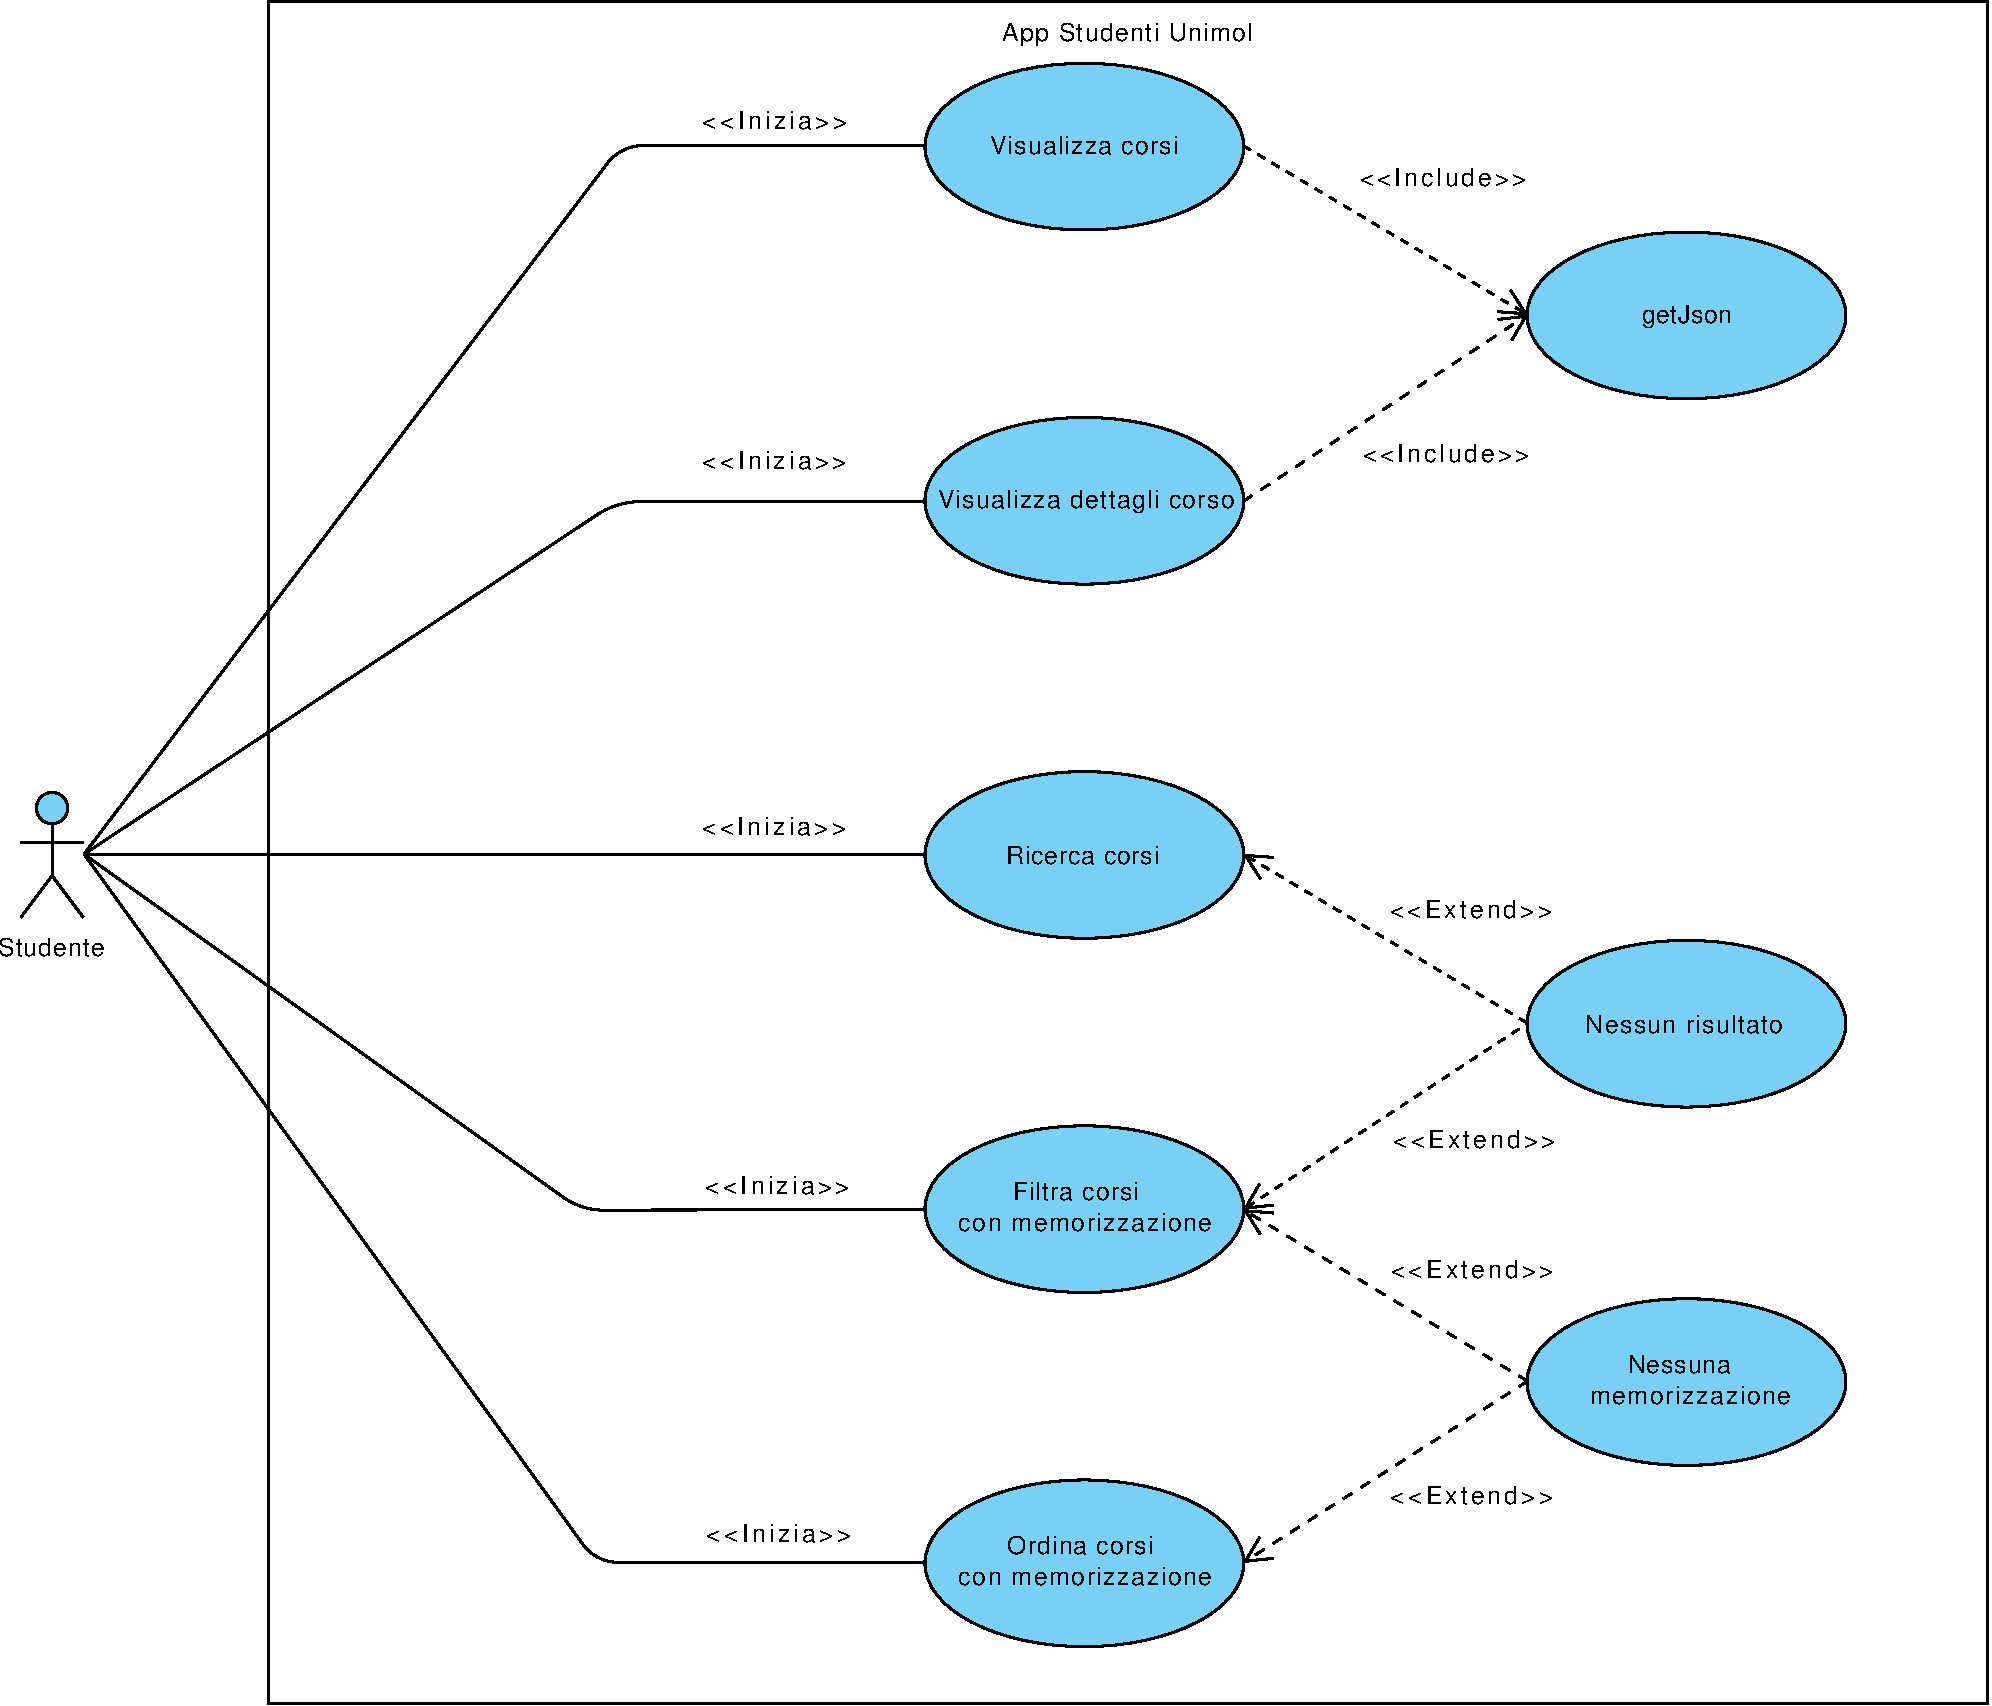
\includegraphics[width=6.5in]{imgs/gruppo1/use_case_diagrams/UCD1-gestione_piano_di_studio.pdf}
\end{center}
\newpage

%% 8.3.2 Appelli %%
\subsection{Gestione appelli}
\begin{center}
	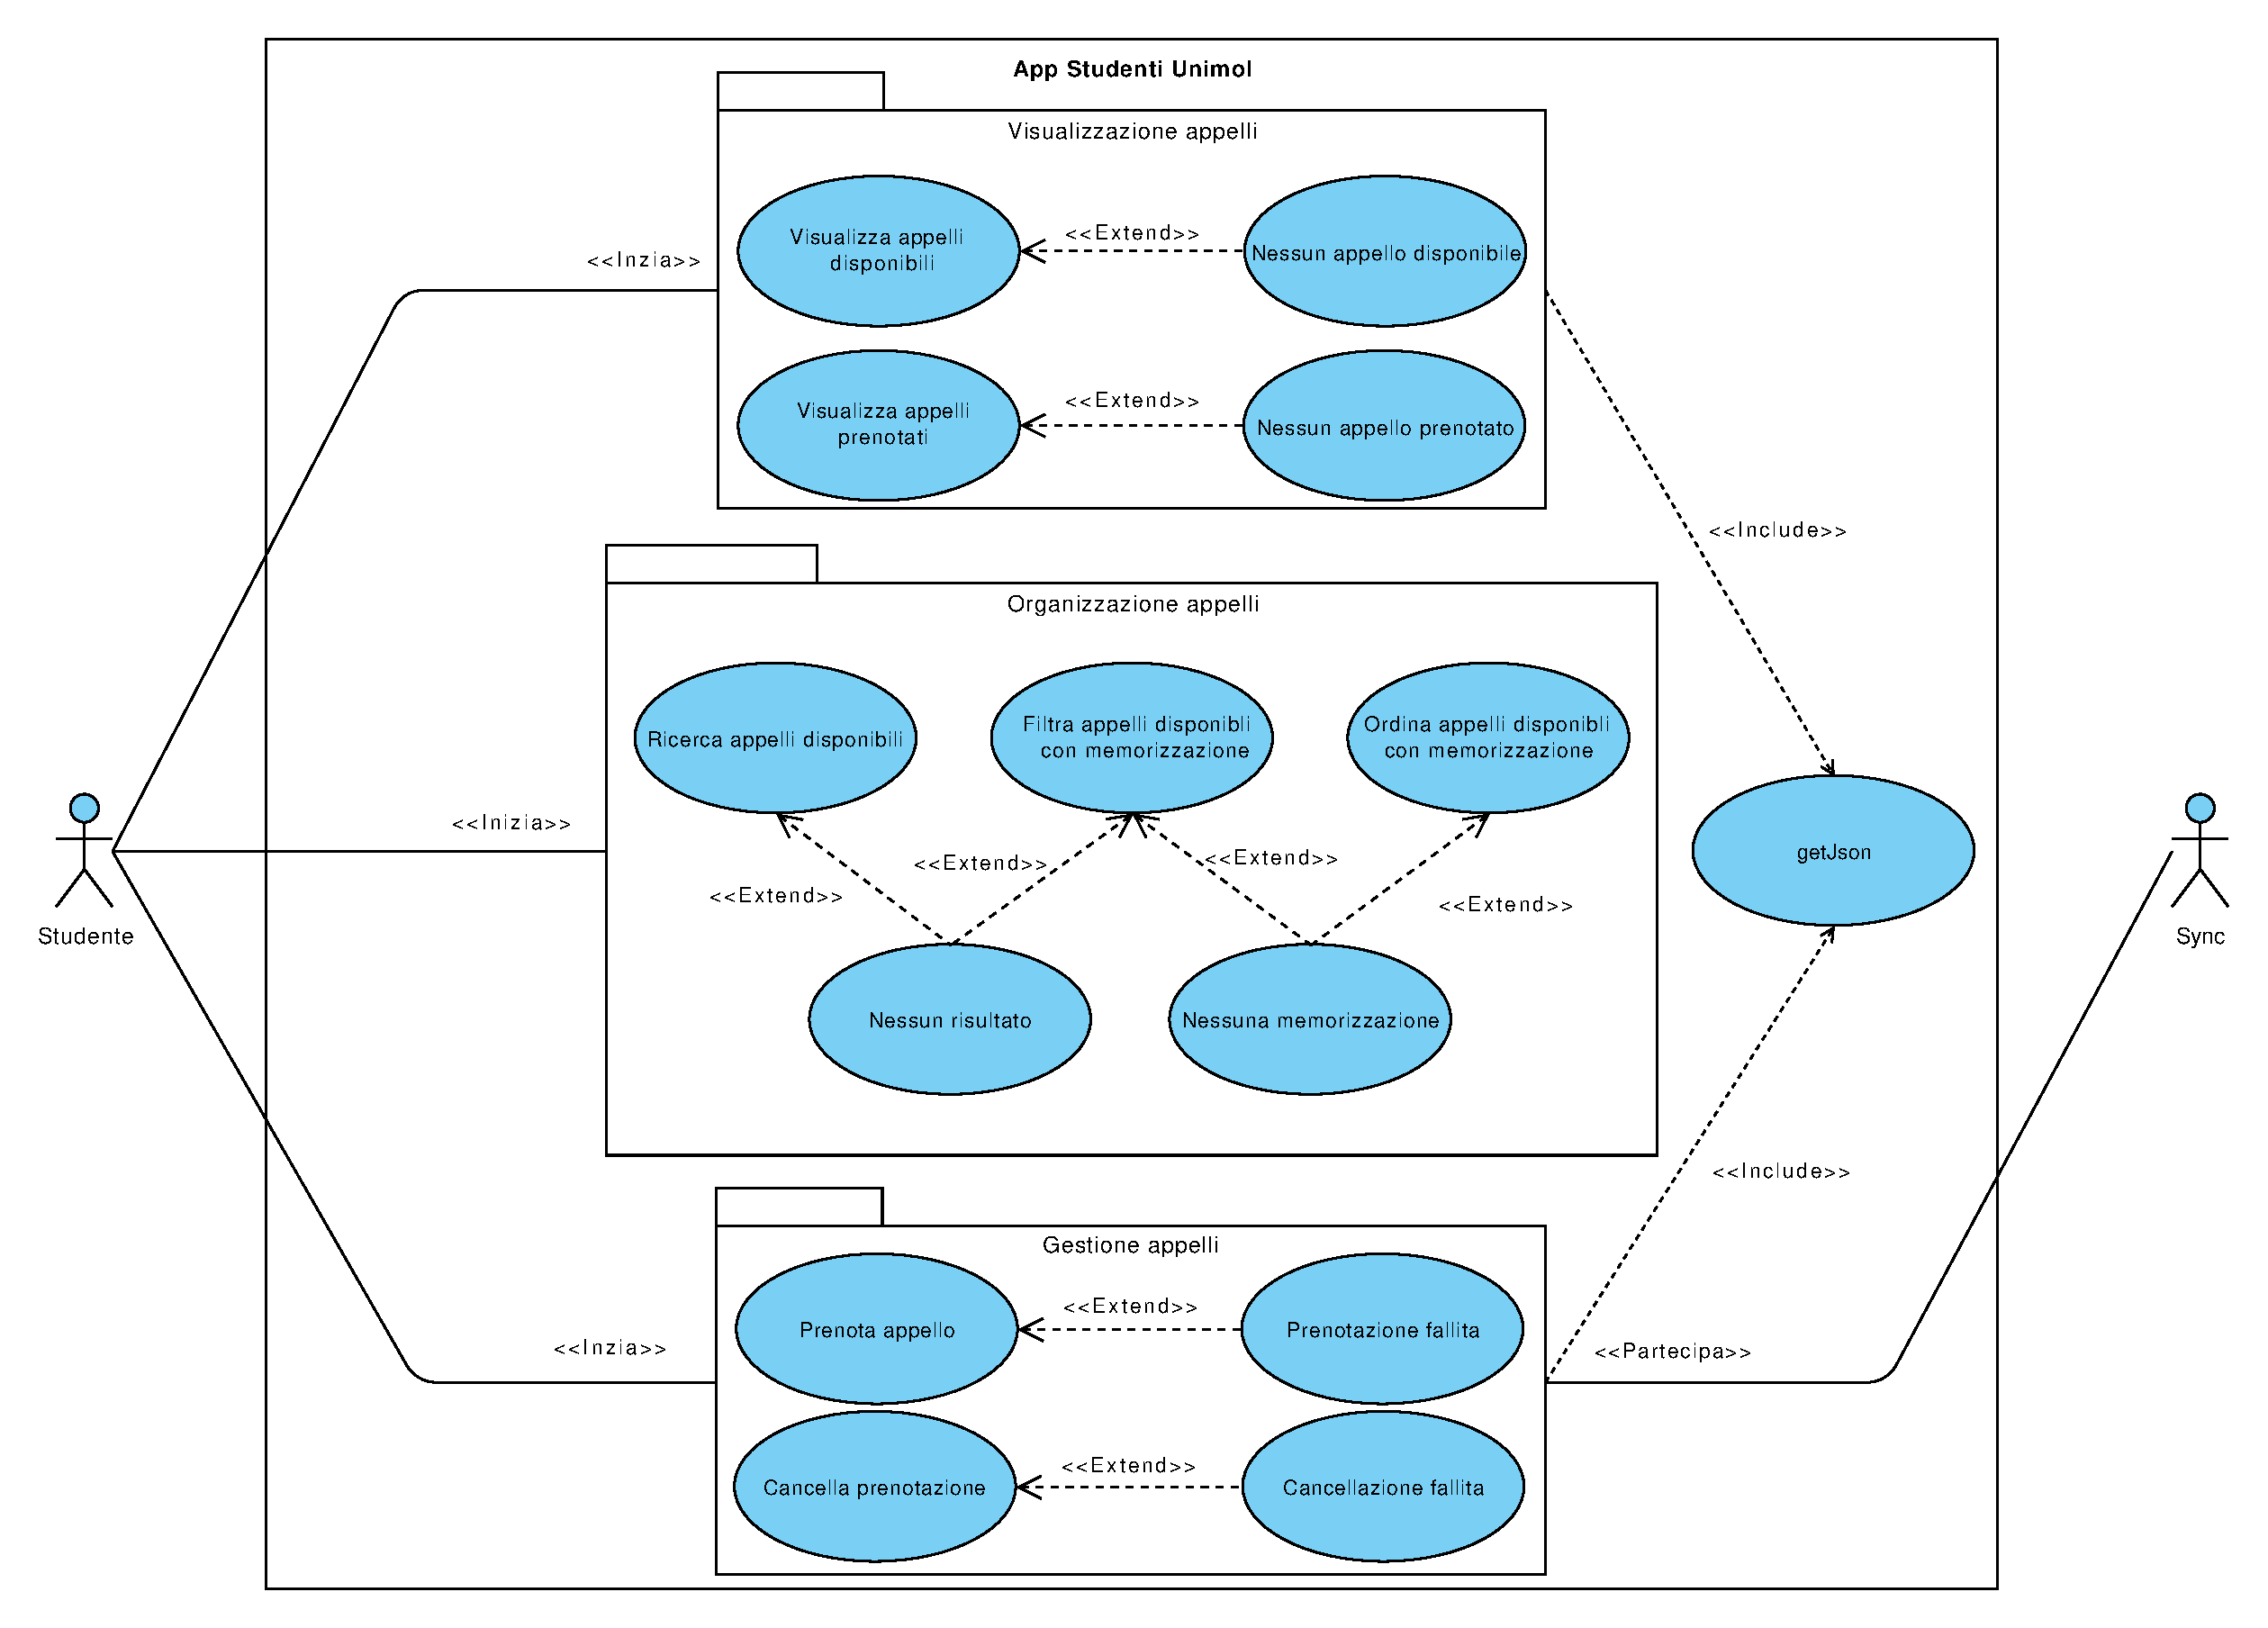
\includegraphics[width=6.5in]{imgs/gruppo1/use_case_diagrams/UCD2-gestione_appelli.pdf}
\end{center}
\newpage

%% 8.3.3 Gestione Materiale Didattico %%
\subsection{Gestione Materiale Didattico}
\begin{center}
	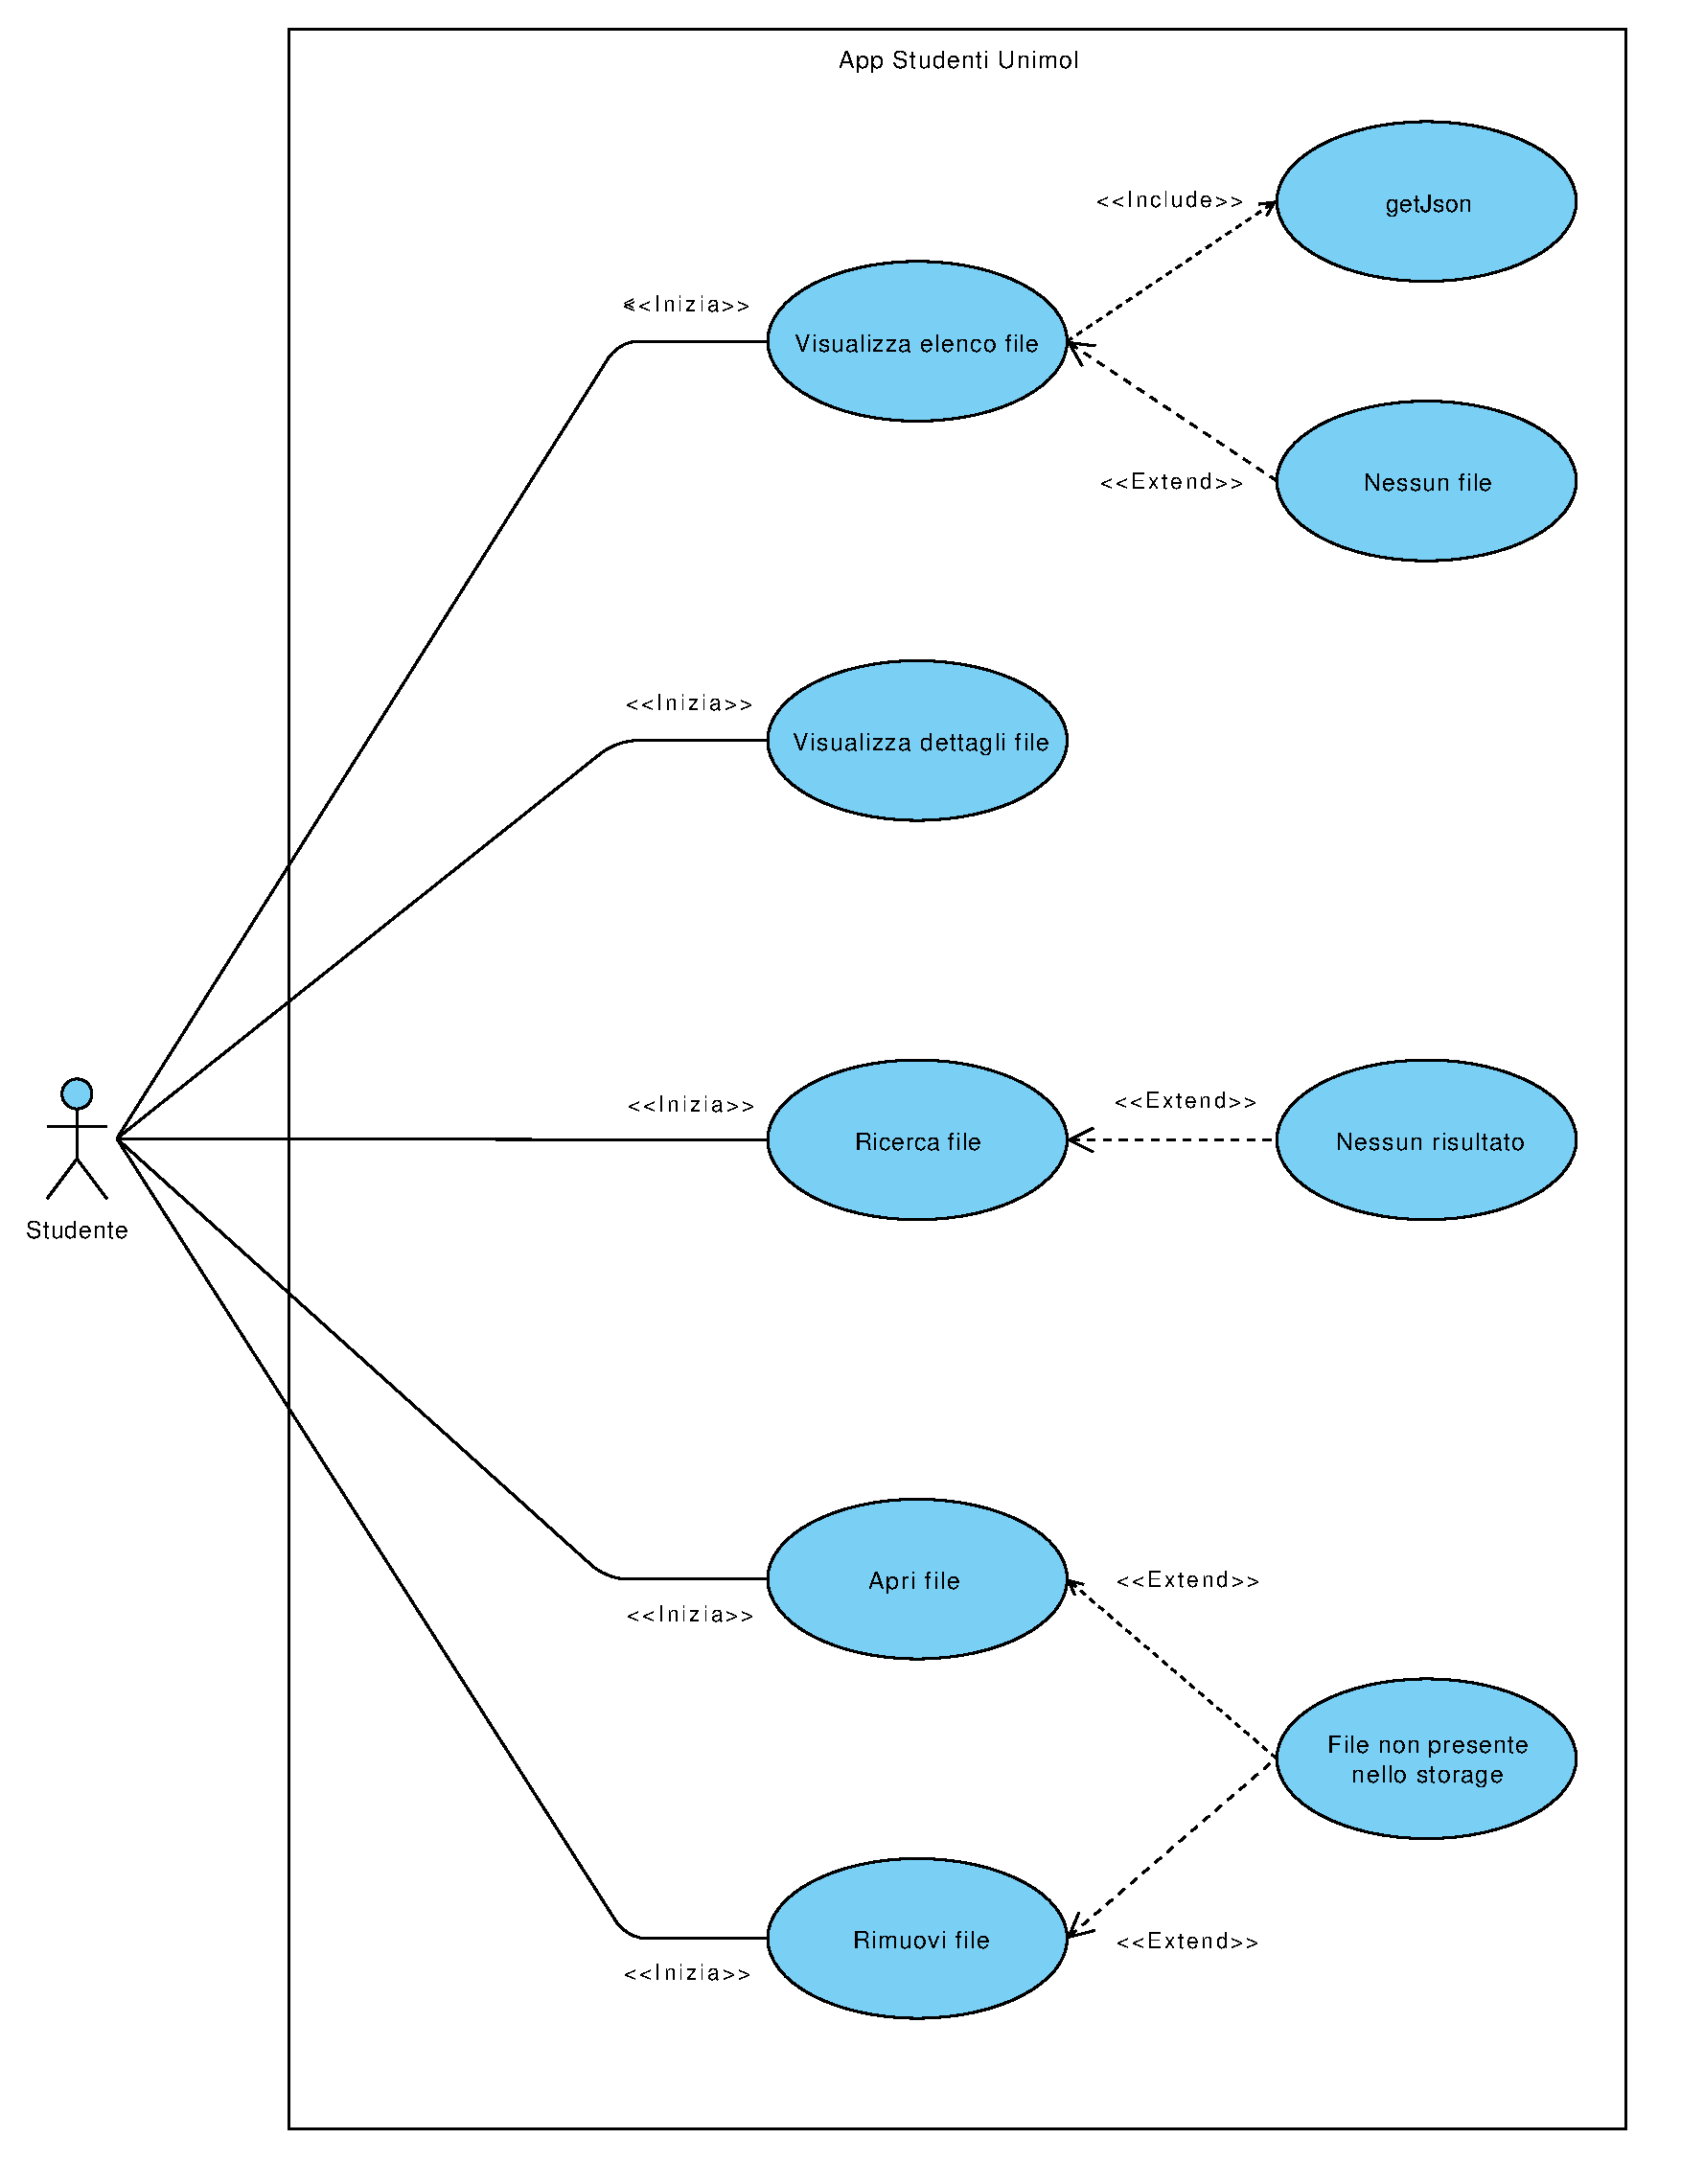
\includegraphics[width=6.5in]{imgs/gruppo1/use_case_diagrams/UCD3-materiale_didattico.pdf}
\end{center}
\newpage




\section{Diagrammi di sequenza}


%%8.5.1 - Visualizza corsi%%
\subsection{Visualizza corsi}
\begin{center}
	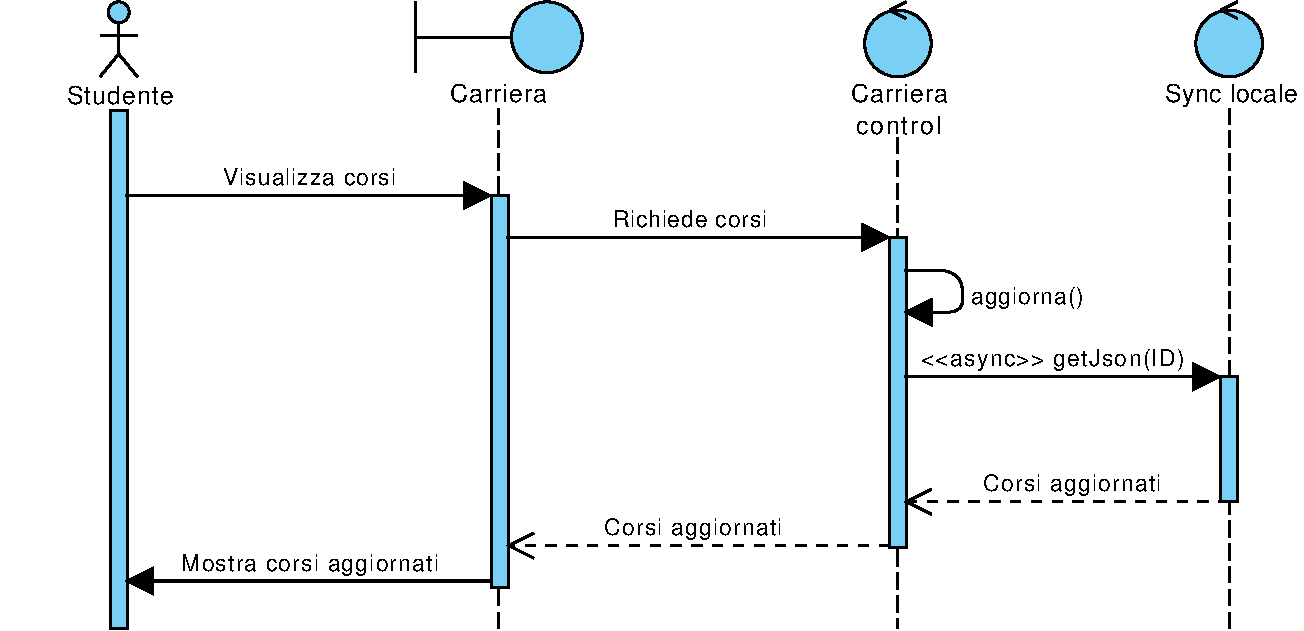
\includegraphics[width=6.5in]{imgs/gruppo1/sequence_diagrams/SD1_visualizza_corsi.pdf}
\end{center}
%%8.5.2 - Ricerca corsi%%
\subsection{Ricerca corsi}
\begin{center}
	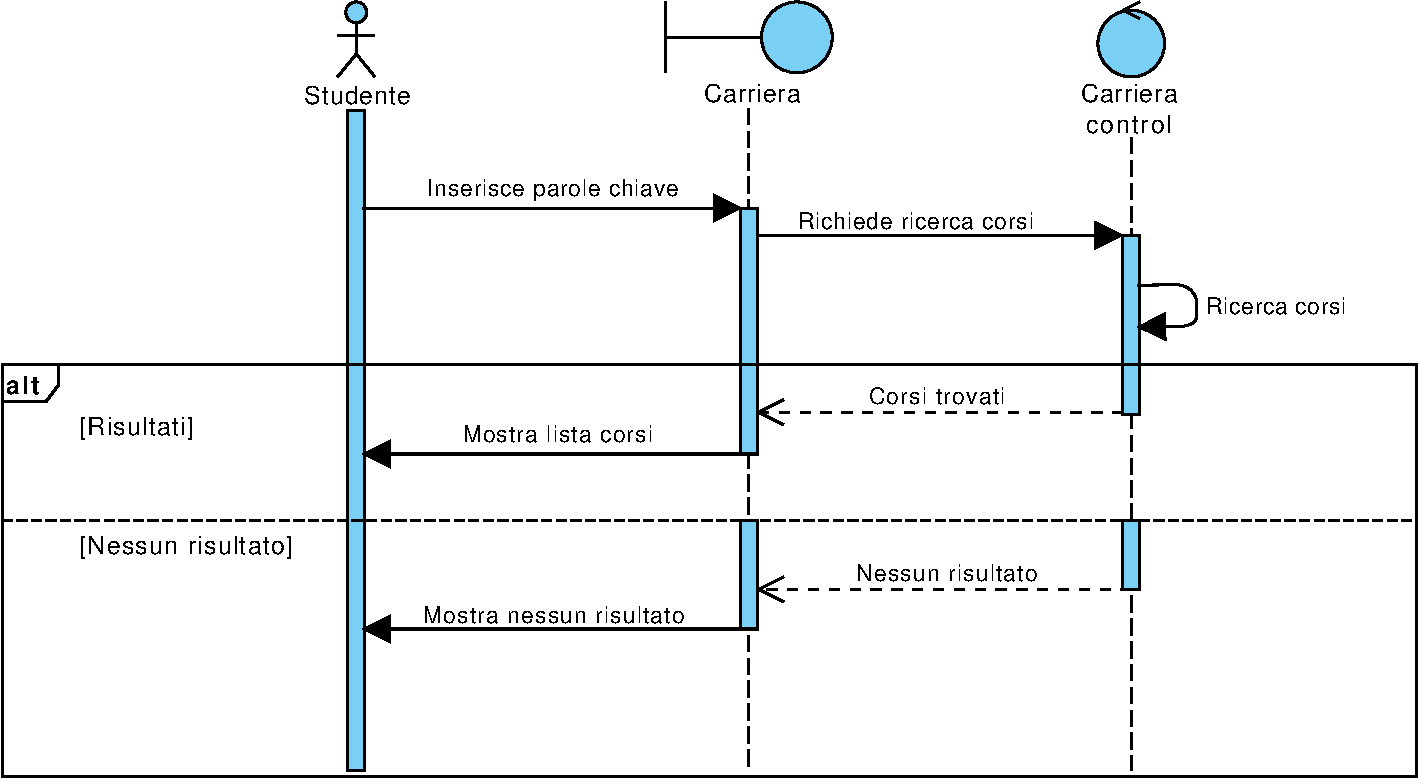
\includegraphics[width=6.5in]{imgs/gruppo1/sequence_diagrams/SD2_ricerca_corsi.pdf}
\end{center}
\newpage


%%8.5.3 - Filtra corsi con memorizzazione%%
\subsection{Filtra corsi con memorizzazione}
\begin{center}
	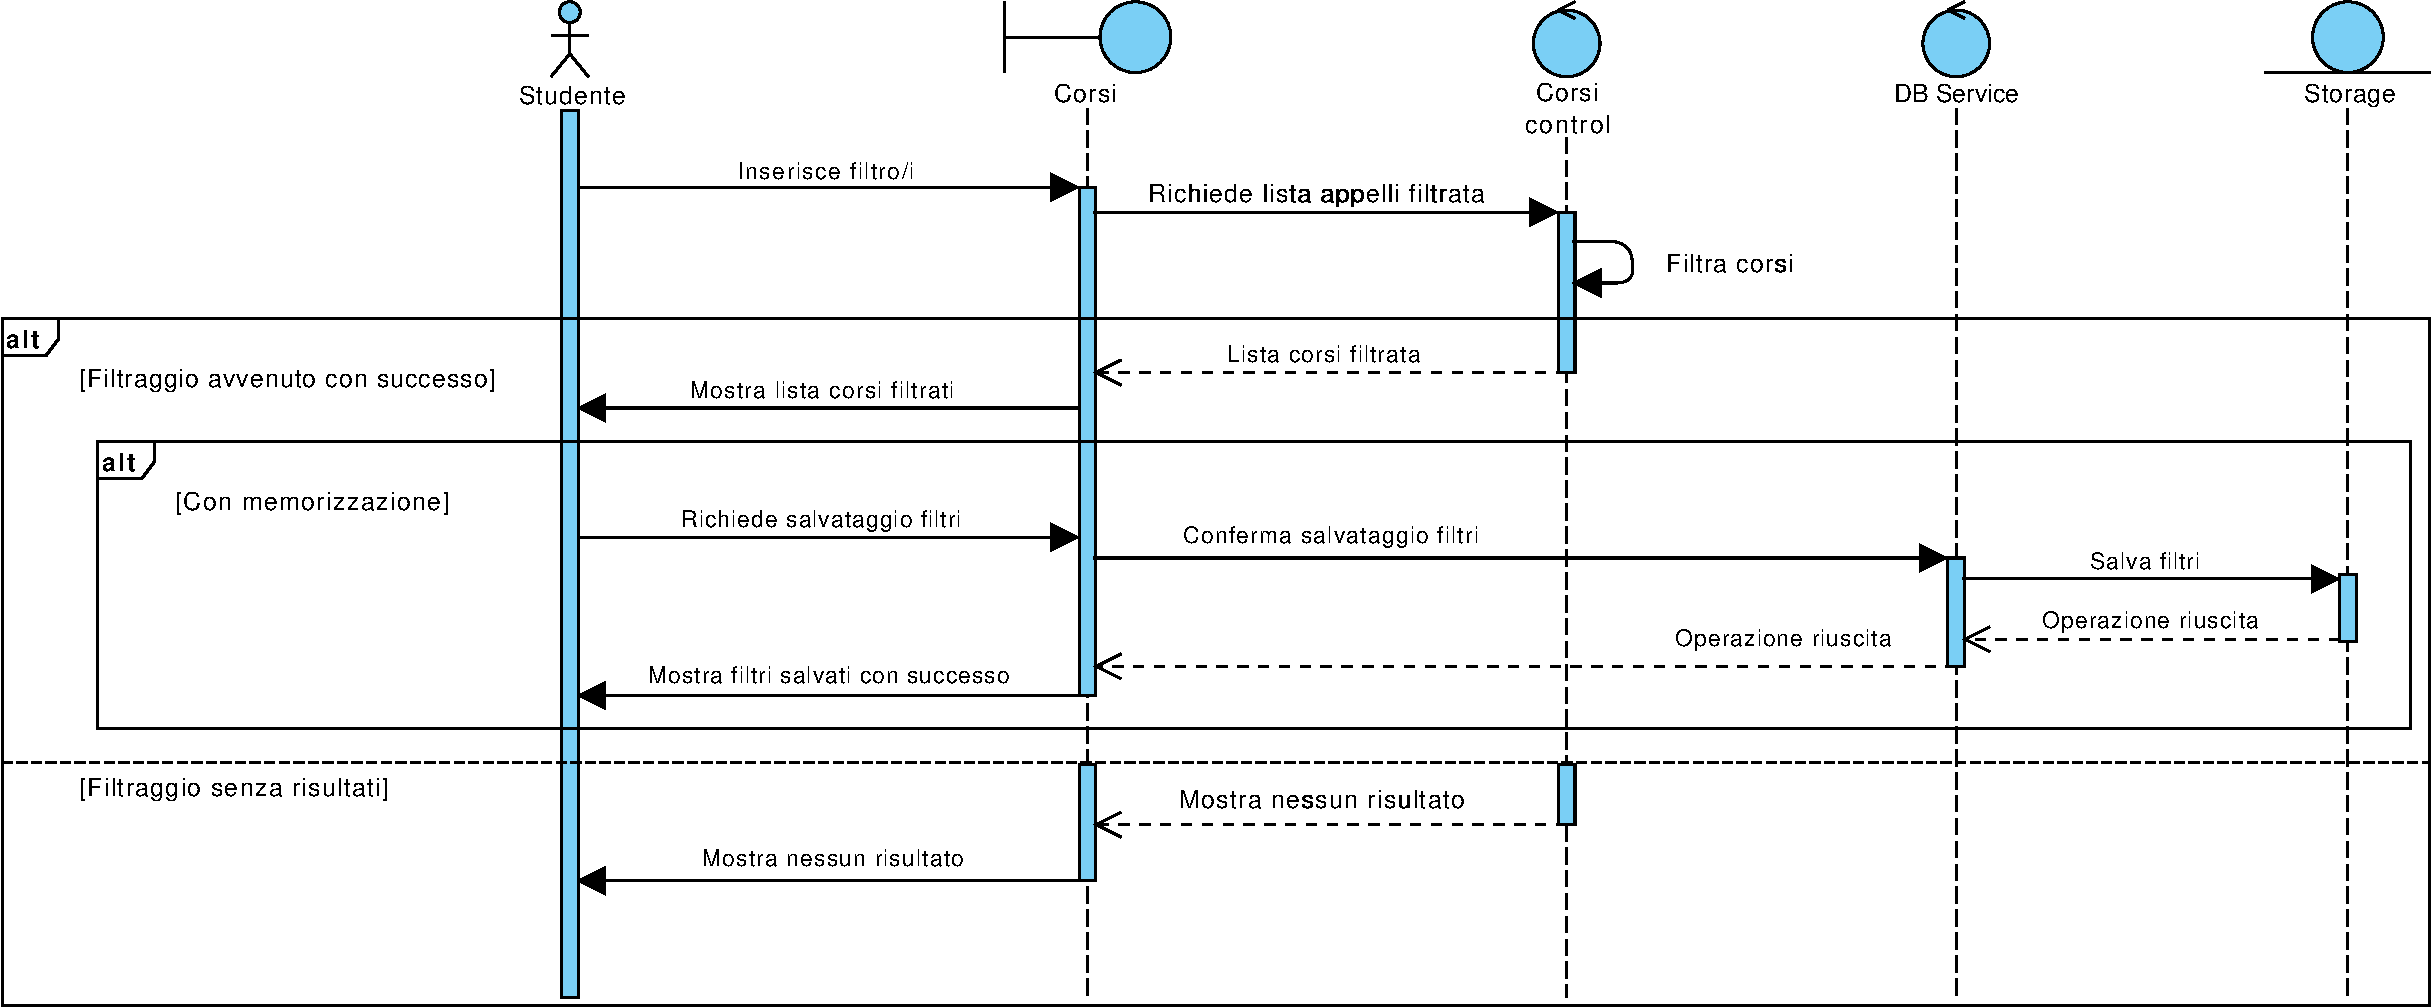
\includegraphics[width=6.5in]{imgs/gruppo1/sequence_diagrams/SD3_filtra_corsi_con_memorizzazione.pdf}
\end{center}
%%8.5.4 - Ordina corsi con memorizzazione%%
\subsection{Ordina corsi con memorizzazione}
\begin{center}
	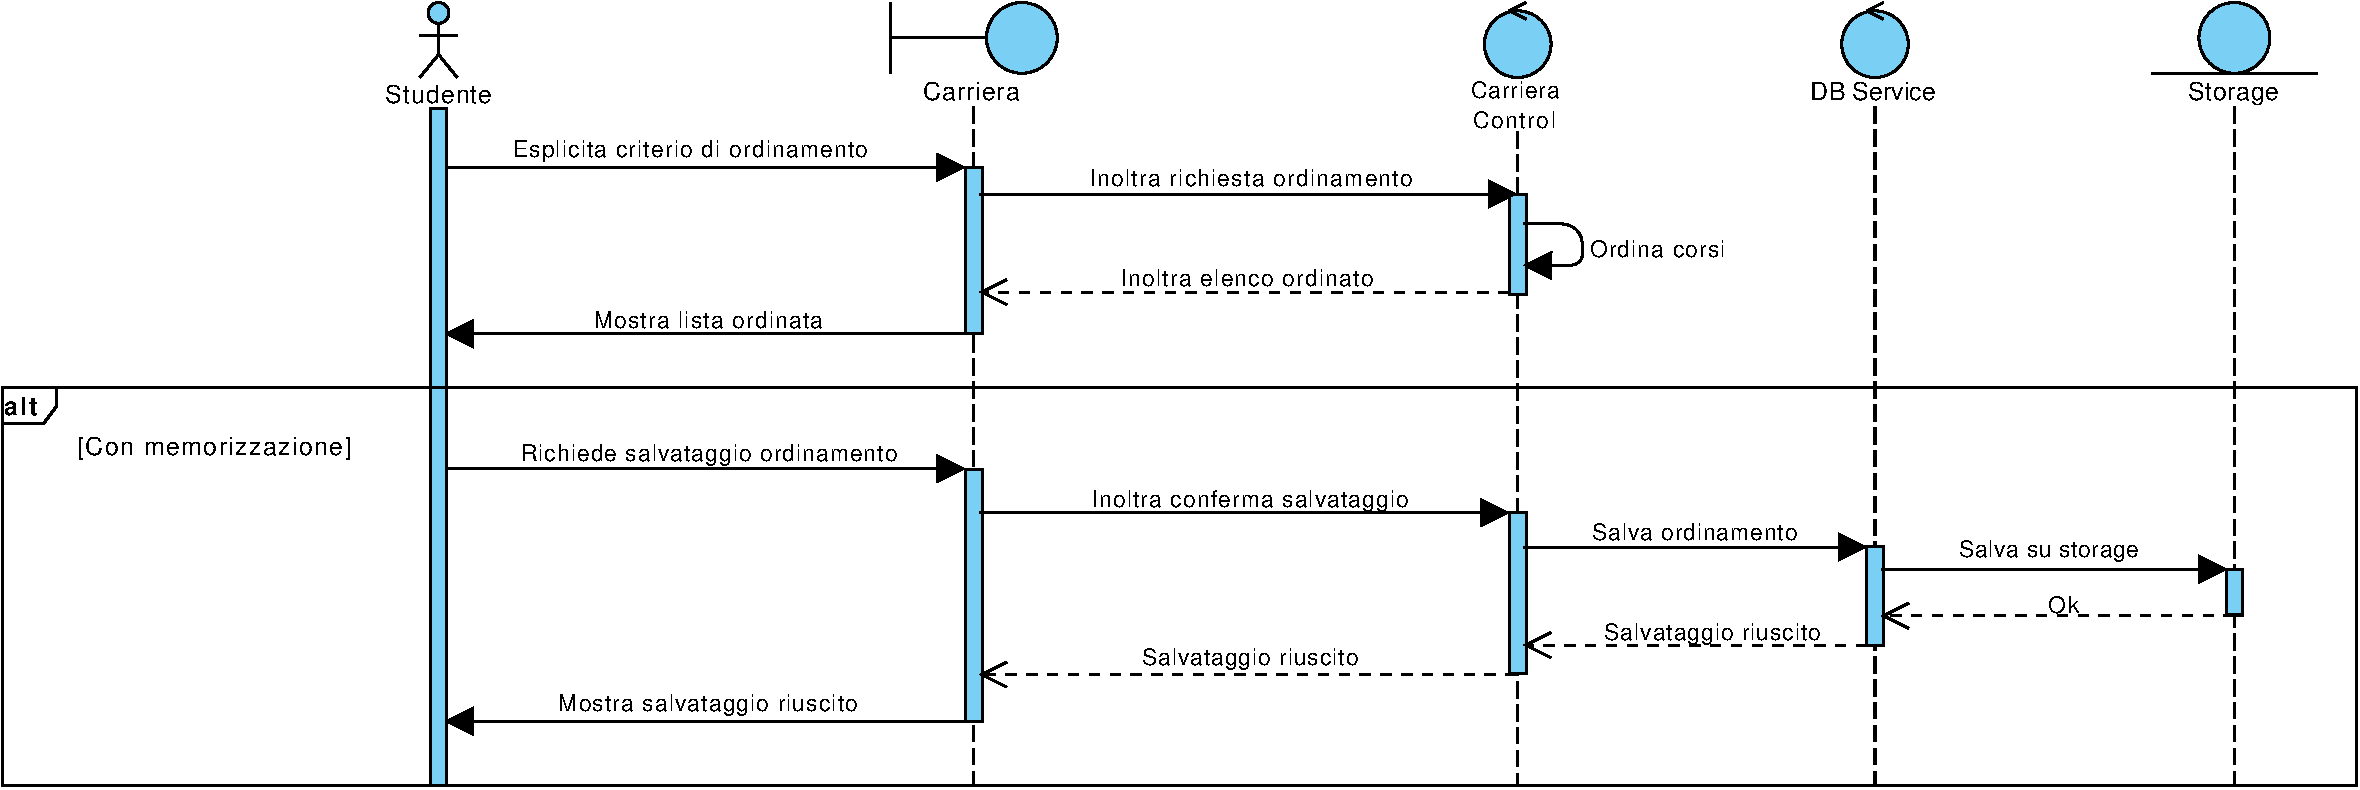
\includegraphics[width=6.5in]{imgs/gruppo1/sequence_diagrams/SD4_ordina_corsi_con_memorizzazione.pdf}
\end{center}
\newpage


%%8.5.5 - Visualizza dettagli corso%%
\subsection{Visualizza dettagli corso}
\begin{center}
	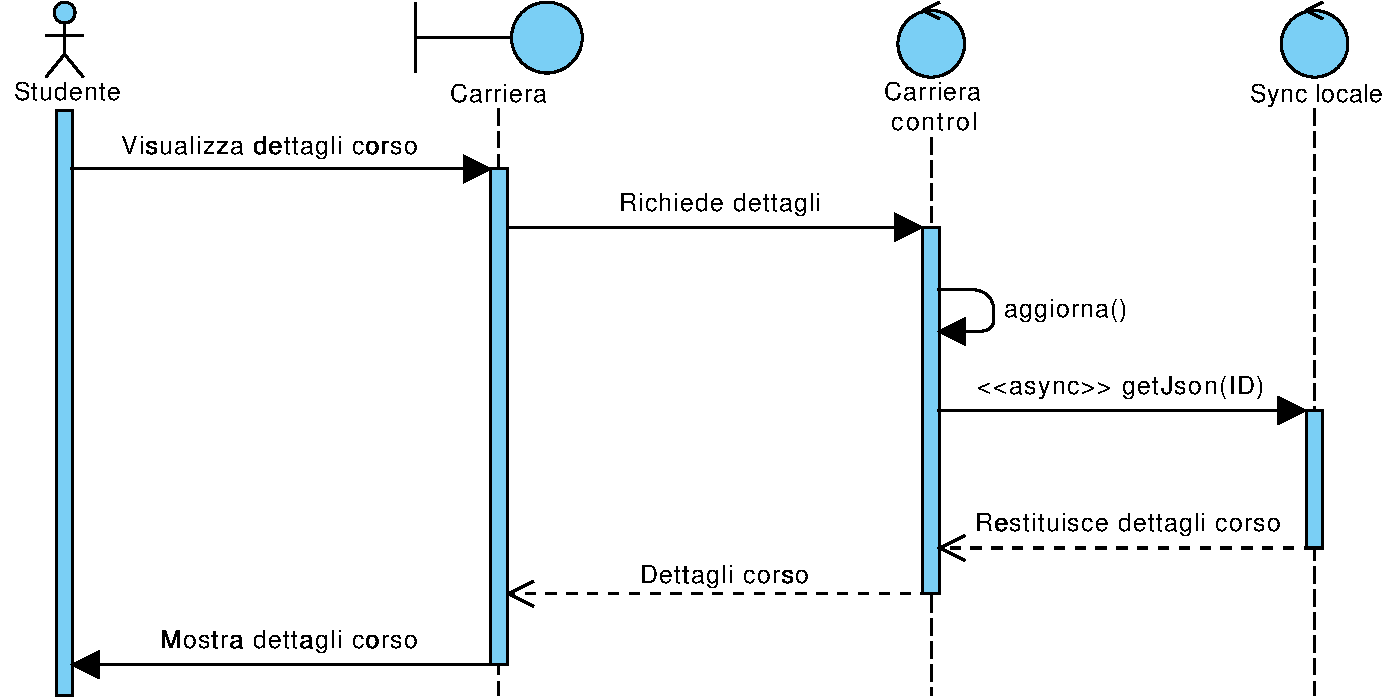
\includegraphics[width=6.5in]{imgs/gruppo1/sequence_diagrams/SD5_visualizza_dettagli_corso.pdf}
\end{center}
%%8.5.6 - Visualizza appelli disponibili %%
\subsection{Visualizza appelli disponibili}
\begin{center}
	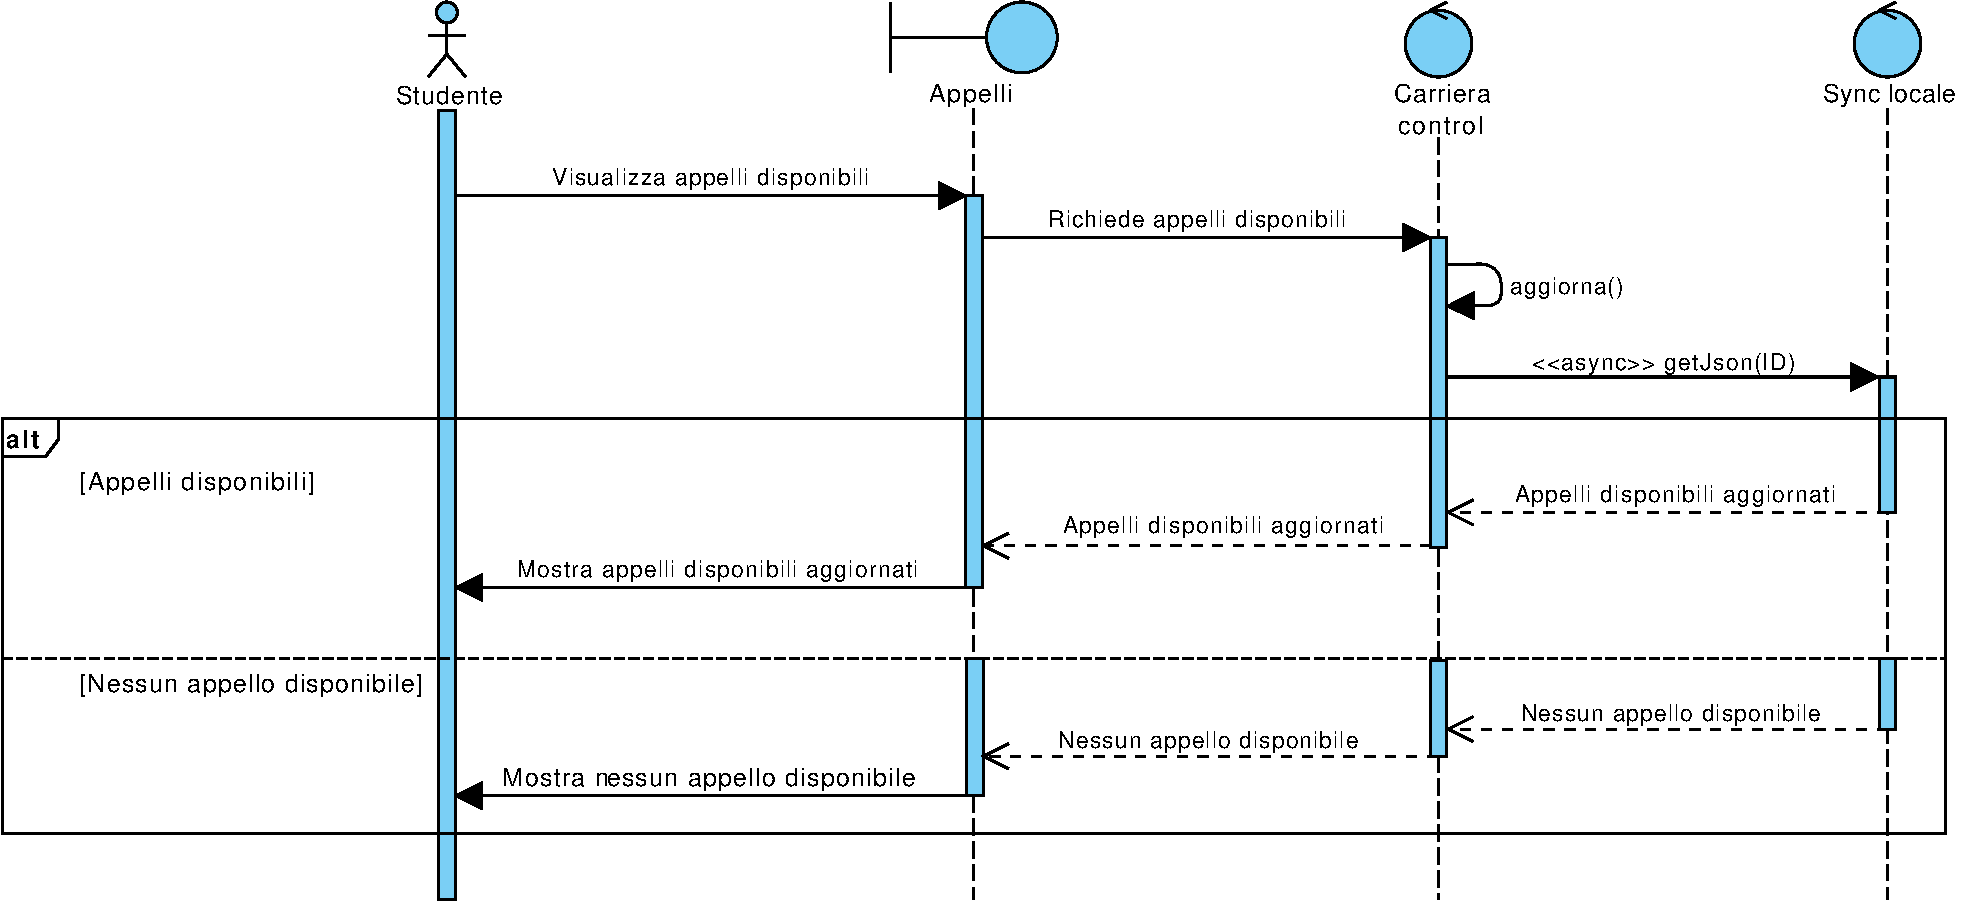
\includegraphics[width=6.5in]{imgs/gruppo1/sequence_diagrams/SD6_visualizza_appelli_disponibili.pdf}
\end{center}
\newpage


%%8.5.7 - Visualizza appelli prenotati  %%
\subsection{Visualizza appelli prenotati}
\begin{center}
	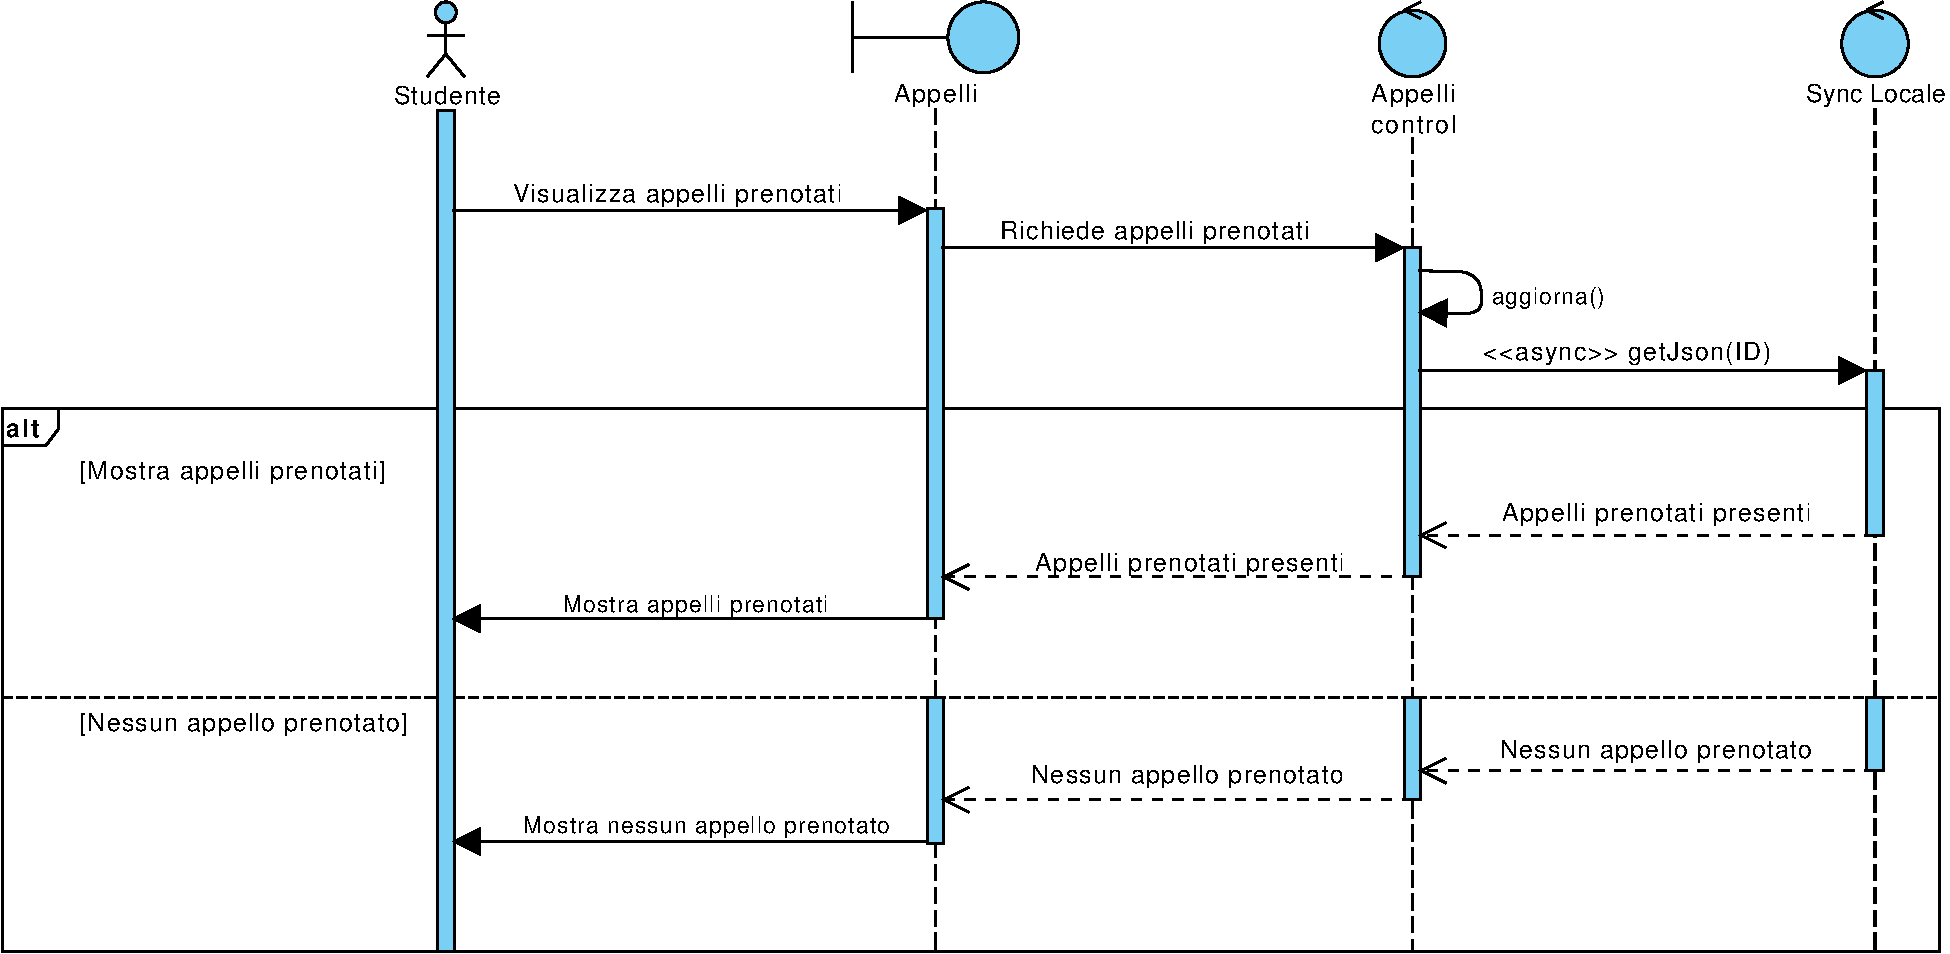
\includegraphics[width=6.5in]{imgs/gruppo1/sequence_diagrams/SD7_visualizza_appelli_prenotati.pdf}
\end{center}
%% 8.5.8 - Ricerca appelli disponibili  %%
\subsection{Ricerca appelli disponibili}
\begin{center}
	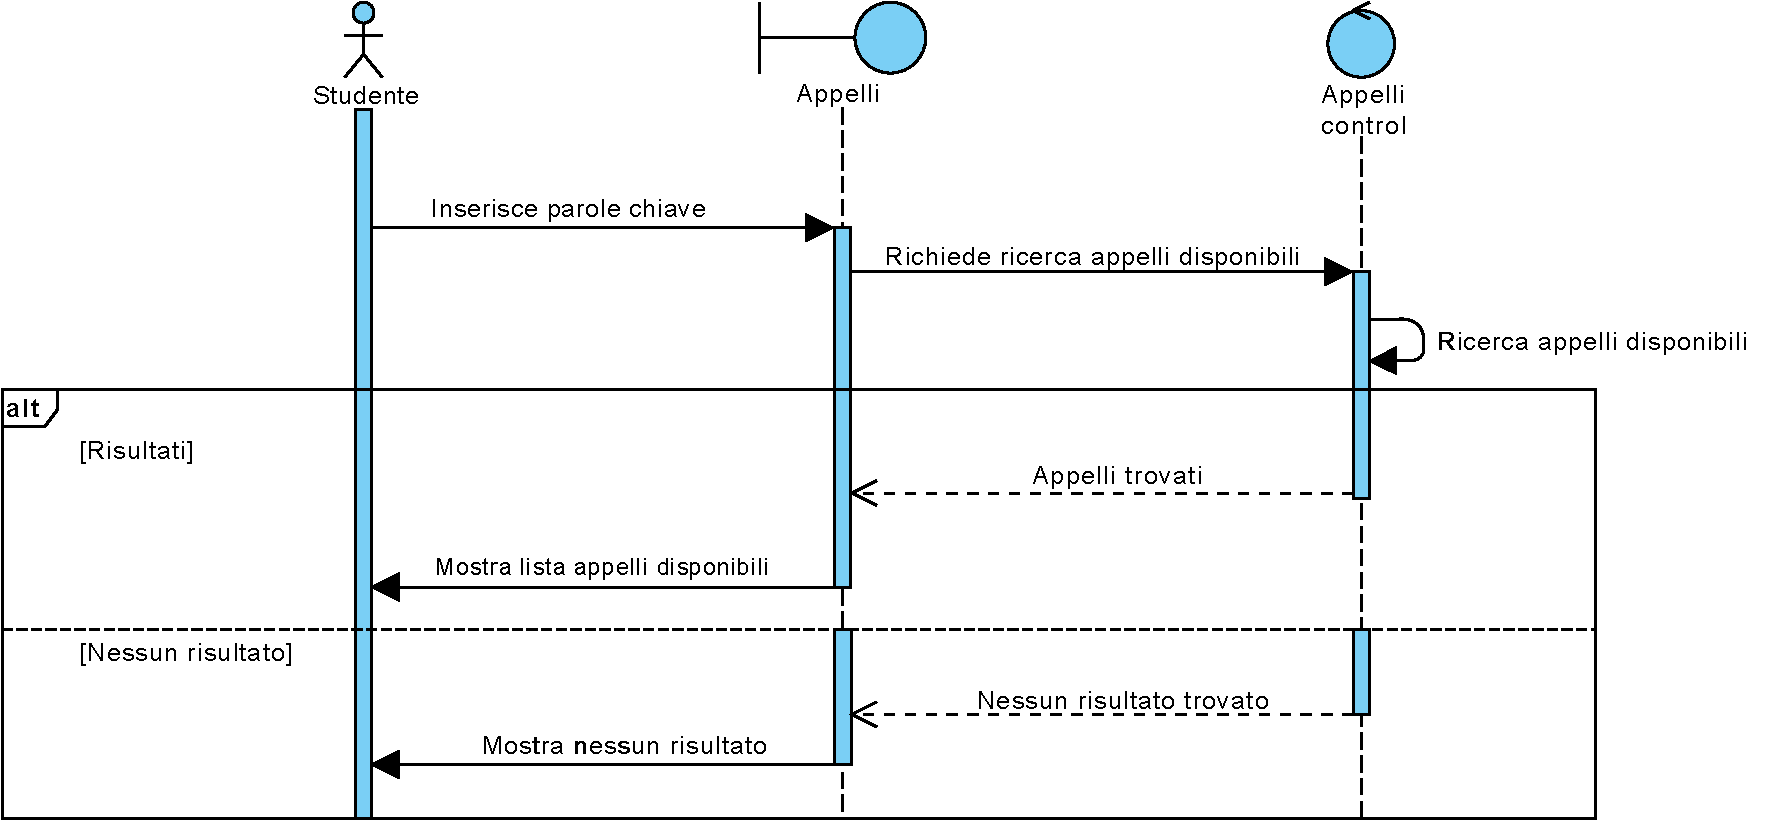
\includegraphics[width=6.5in]{imgs/gruppo1/sequence_diagrams/SD8_ricerca_appelli_disponibili.pdf}
\end{center}
\newpage


%% 8.5.9 - Filtra appelli disponibili con memorizzazione  %%
\subsection{Filtra appelli disponibili con memorizzazione}
\begin{center}
	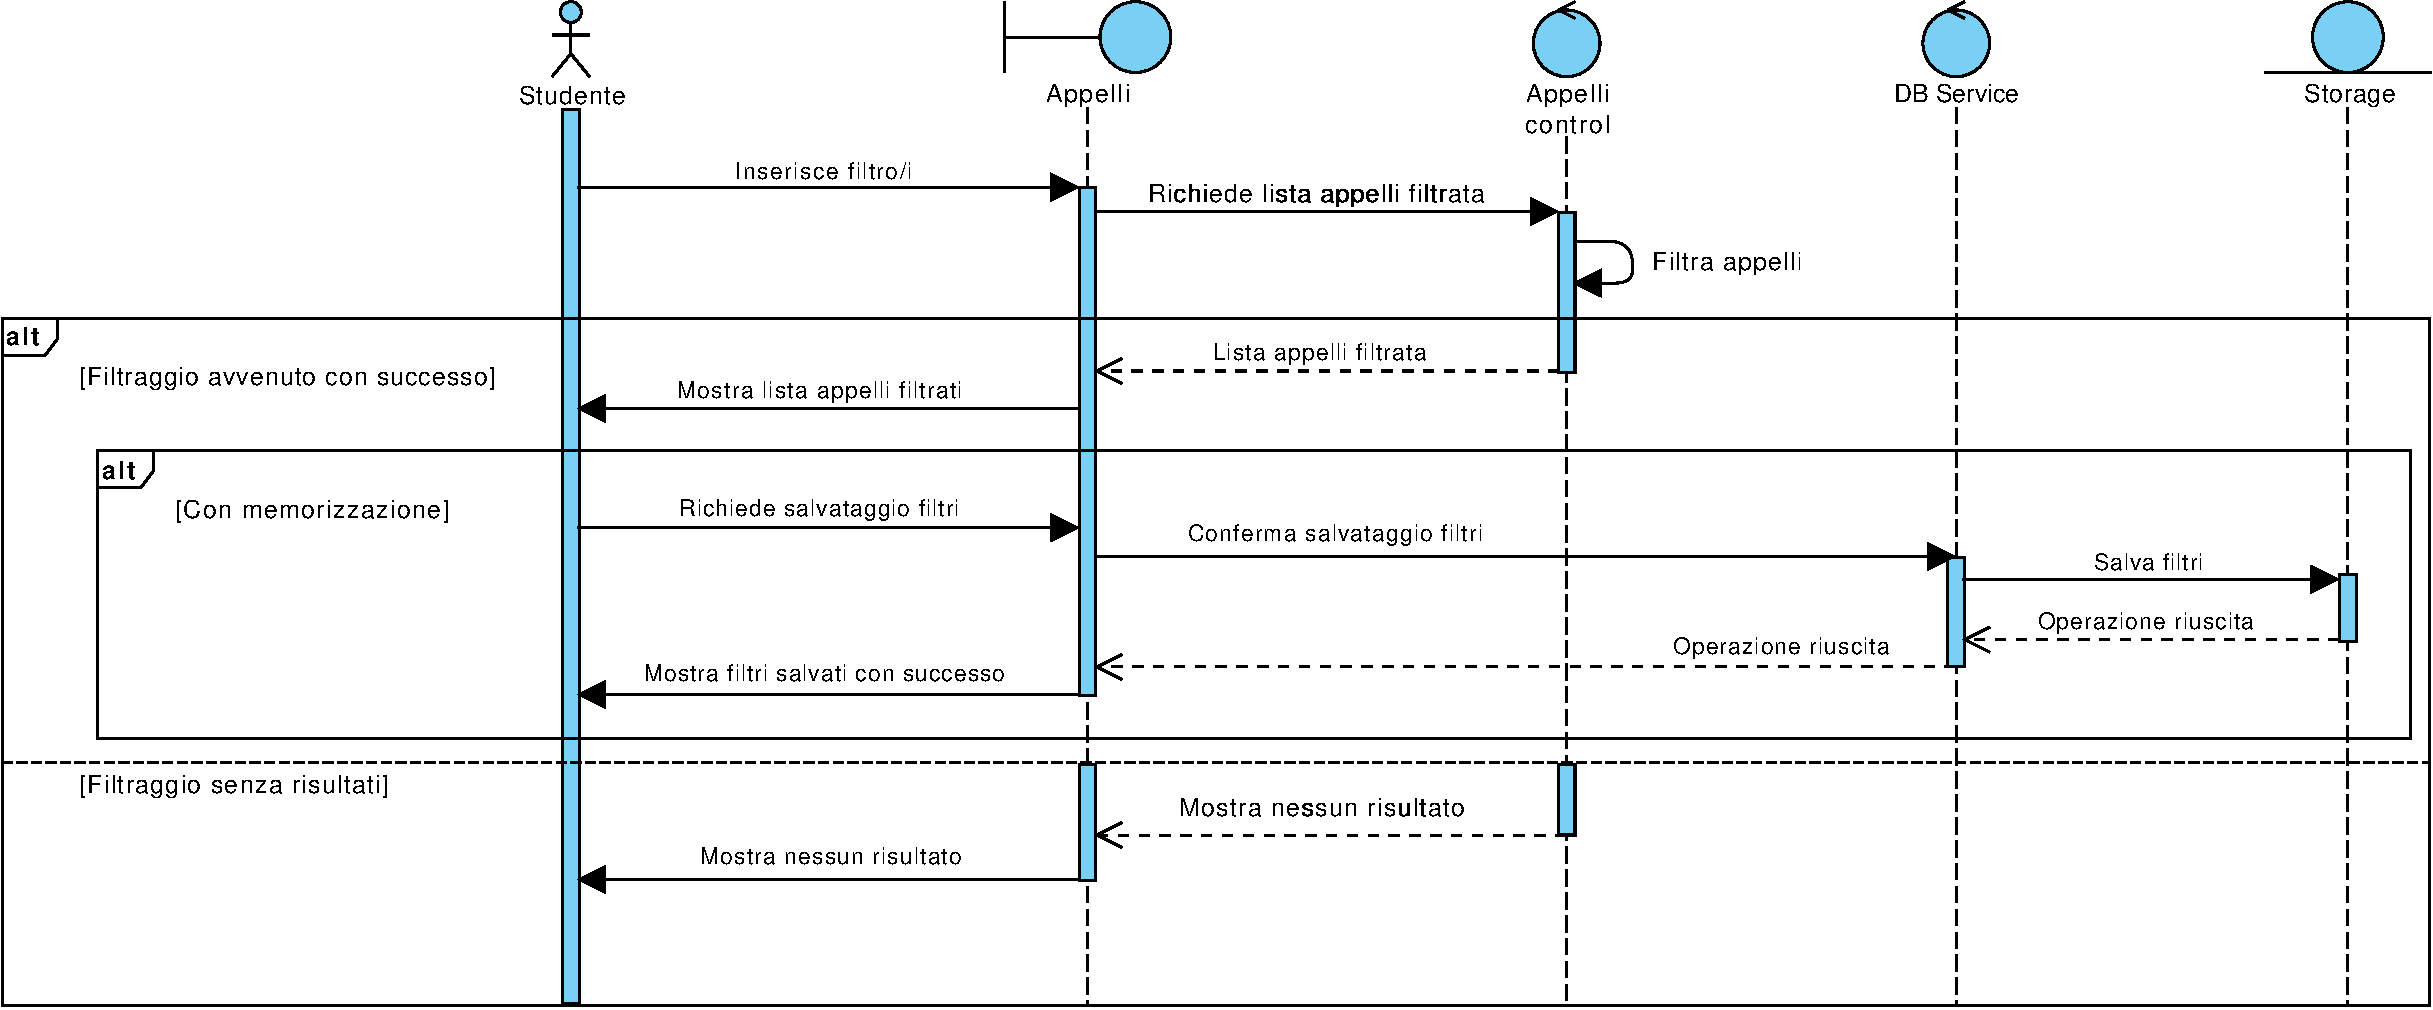
\includegraphics[width=6.5in]{imgs/gruppo1/sequence_diagrams/SD9_filtra_appelli_disponibili_con_memorizzazione.pdf}
\end{center}
%% 8.5.10 - Ordina appelli disponibili con memorizzazione  %%
\subsection{Ordina appelli disponibili con memorizzazione}
\begin{center}
	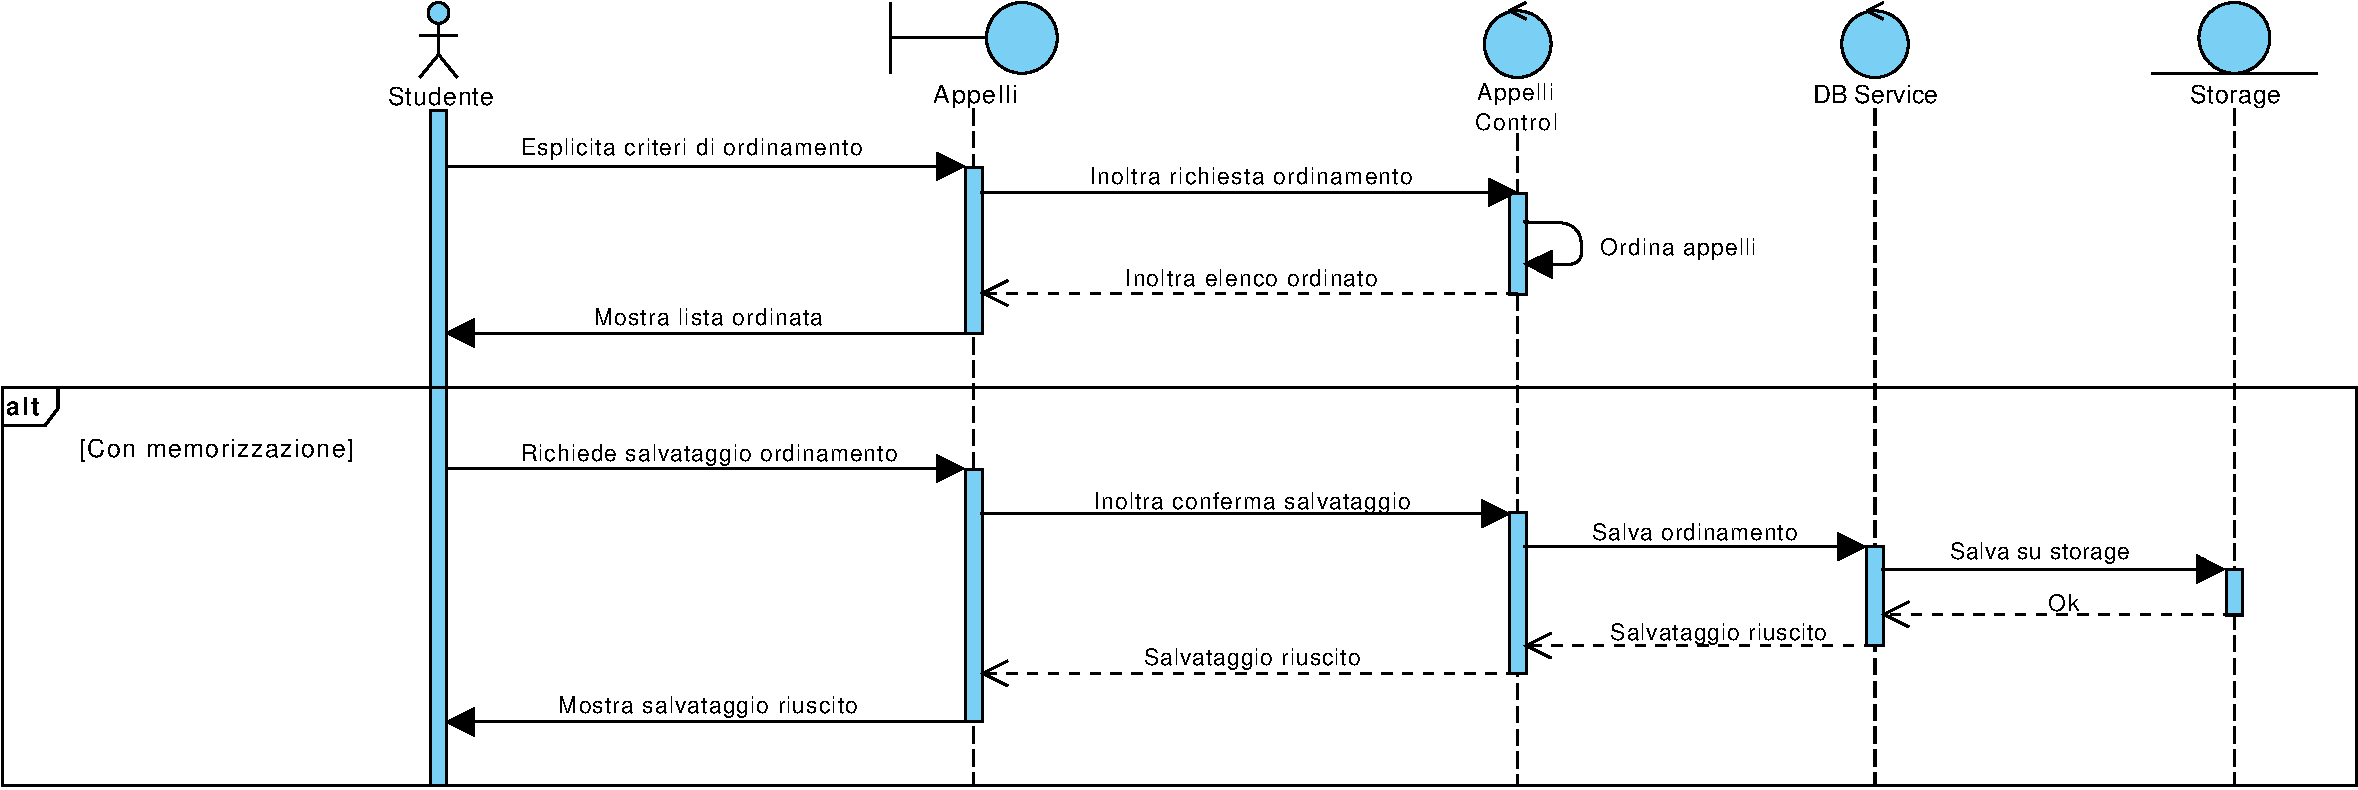
\includegraphics[width=6.5in]{imgs/gruppo1/sequence_diagrams/SD10_ordina_appelli_disponibili_con_memorizzazione.pdf}
\end{center}
\newpage

%%  8.5.11 - Prenota appello  %%
\subsection{Prenota appello}
\begin{center}
	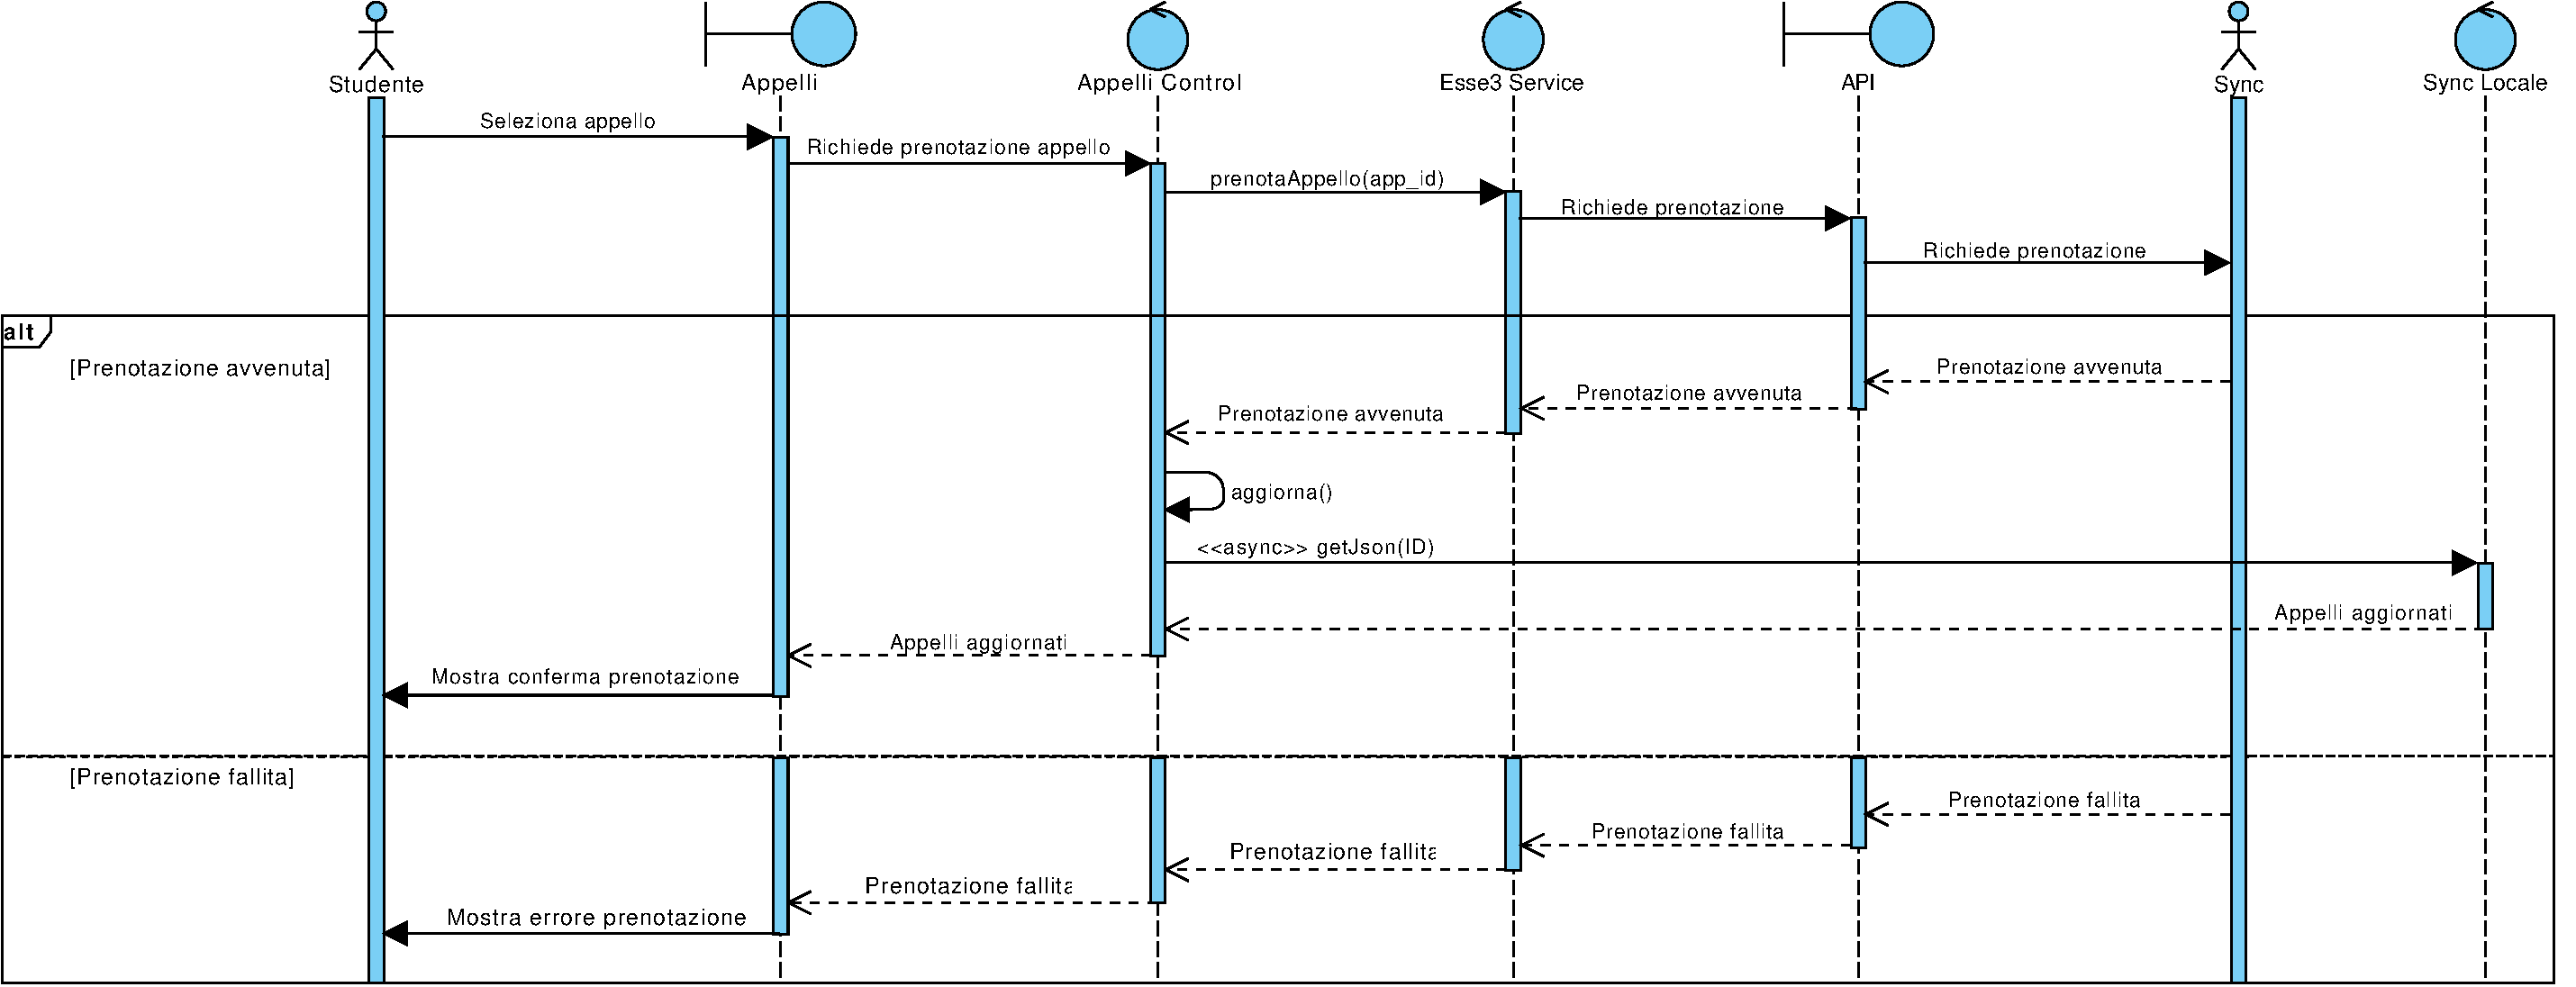
\includegraphics[width=6.5in]{imgs/gruppo1/sequence_diagrams/SD11_prenota_appello.pdf}
\end{center}
%% 8.5.12 - Cancella prenotazione   %%
\subsection{Cancella prenotazione}
\begin{center}
	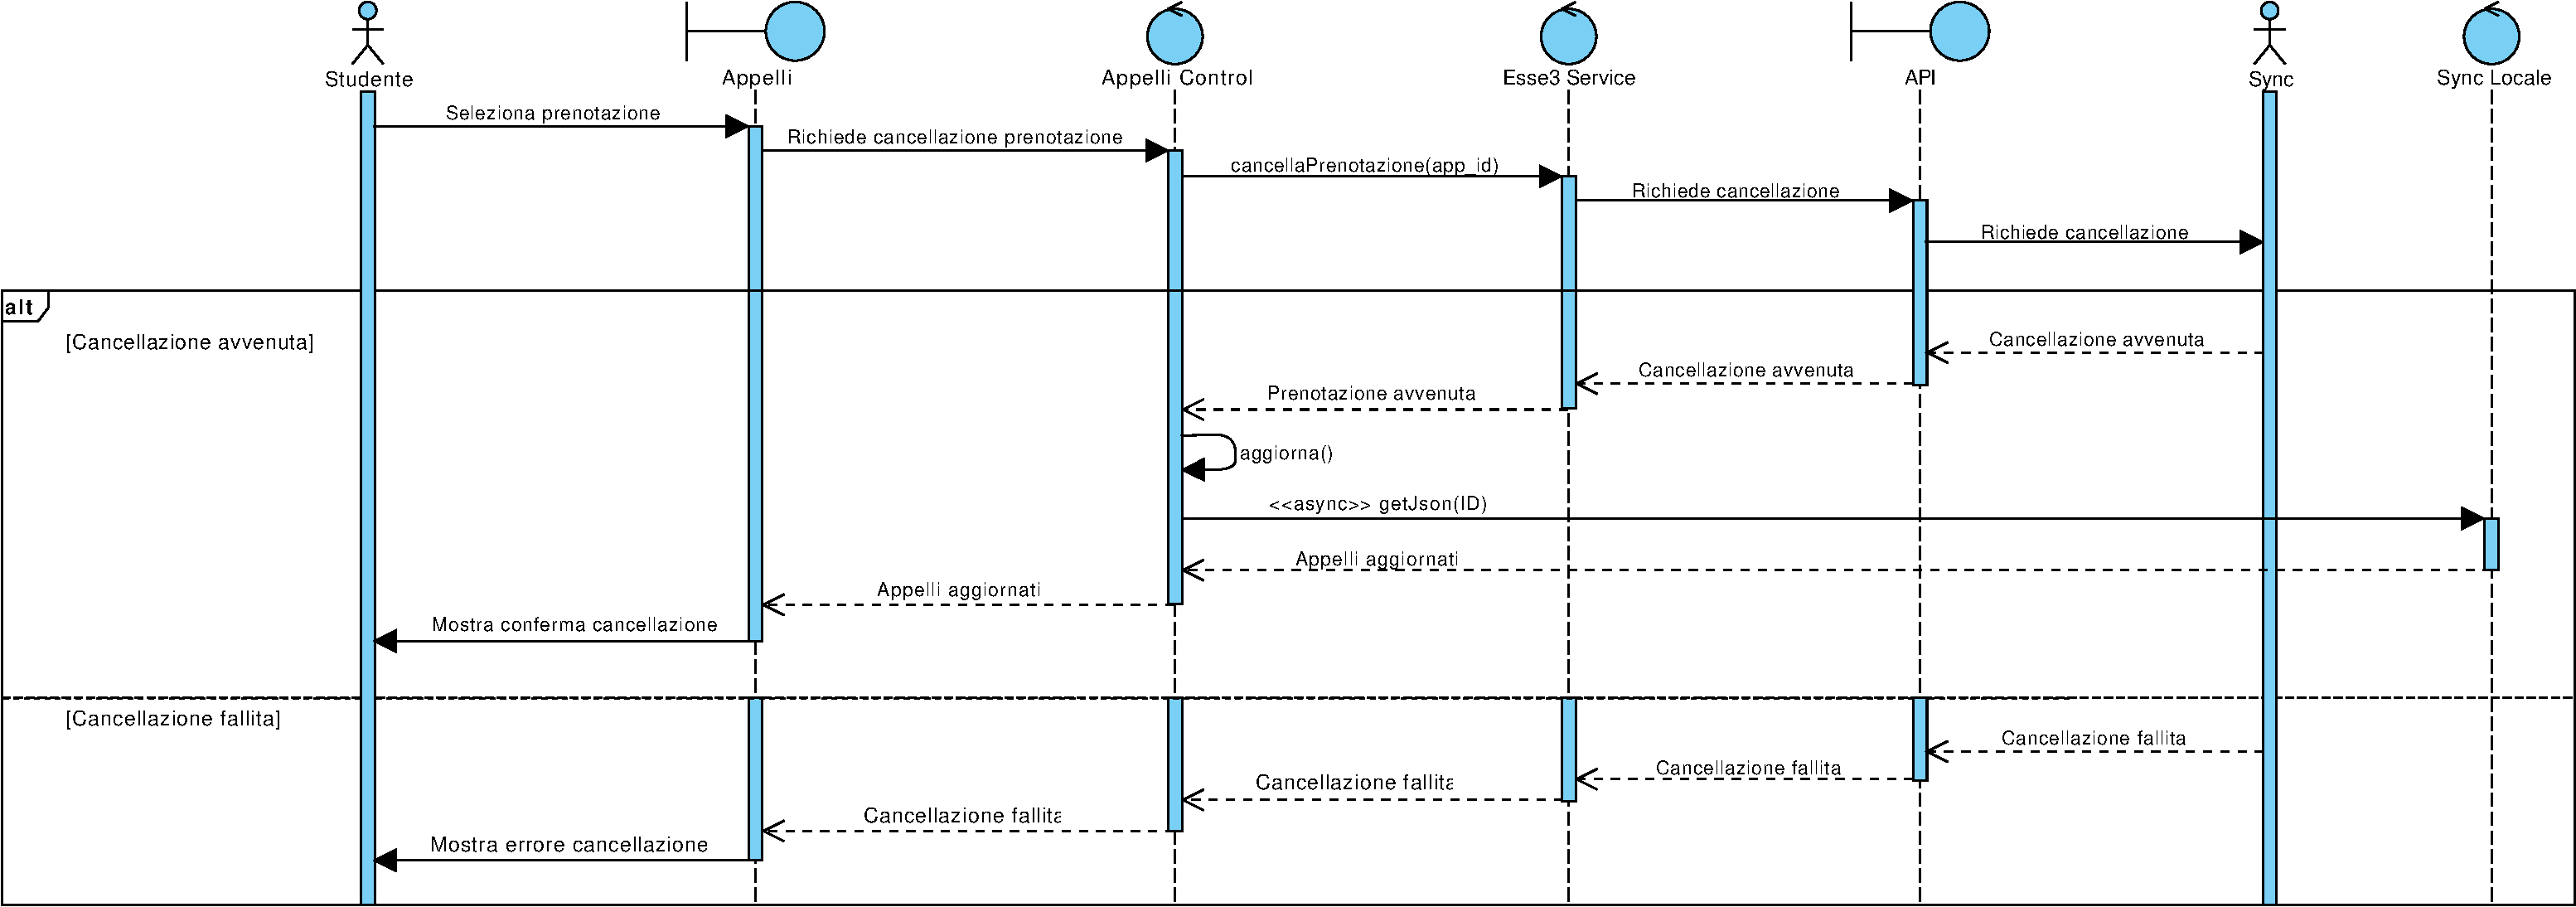
\includegraphics[width=6.5in]{imgs/gruppo1/sequence_diagrams/SD12_cancella_prenotazione.pdf}
\end{center}
\newpage


%%  8.5.13 - Visualizza elenco file  %%
\subsection{Visualizza elenco file}
\begin{center}
	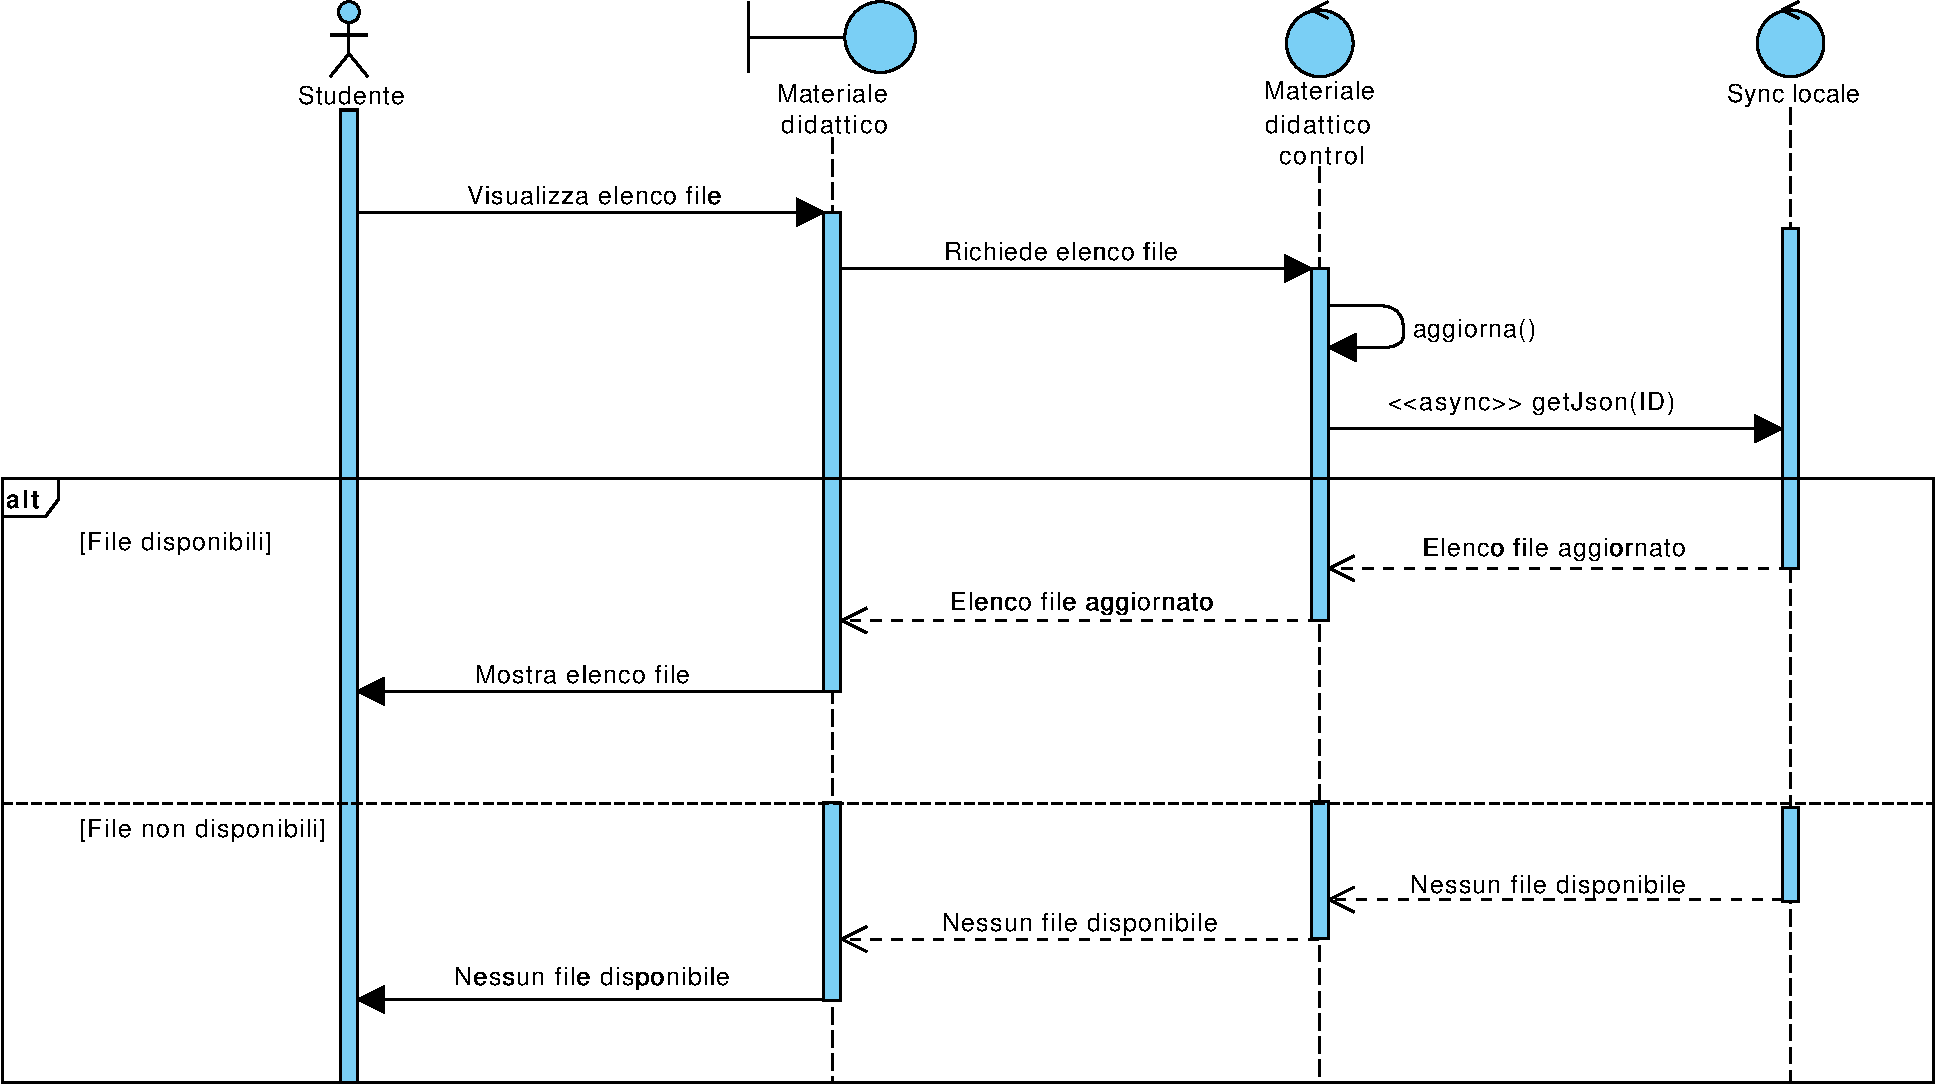
\includegraphics[width=6.5in]{imgs/gruppo1/sequence_diagrams/SD13_visualizza_elenco_file.pdf}
\end{center}
%% 8.5.14 - Ricerca file %
\subsection{Ricerca file}
\begin{center}
	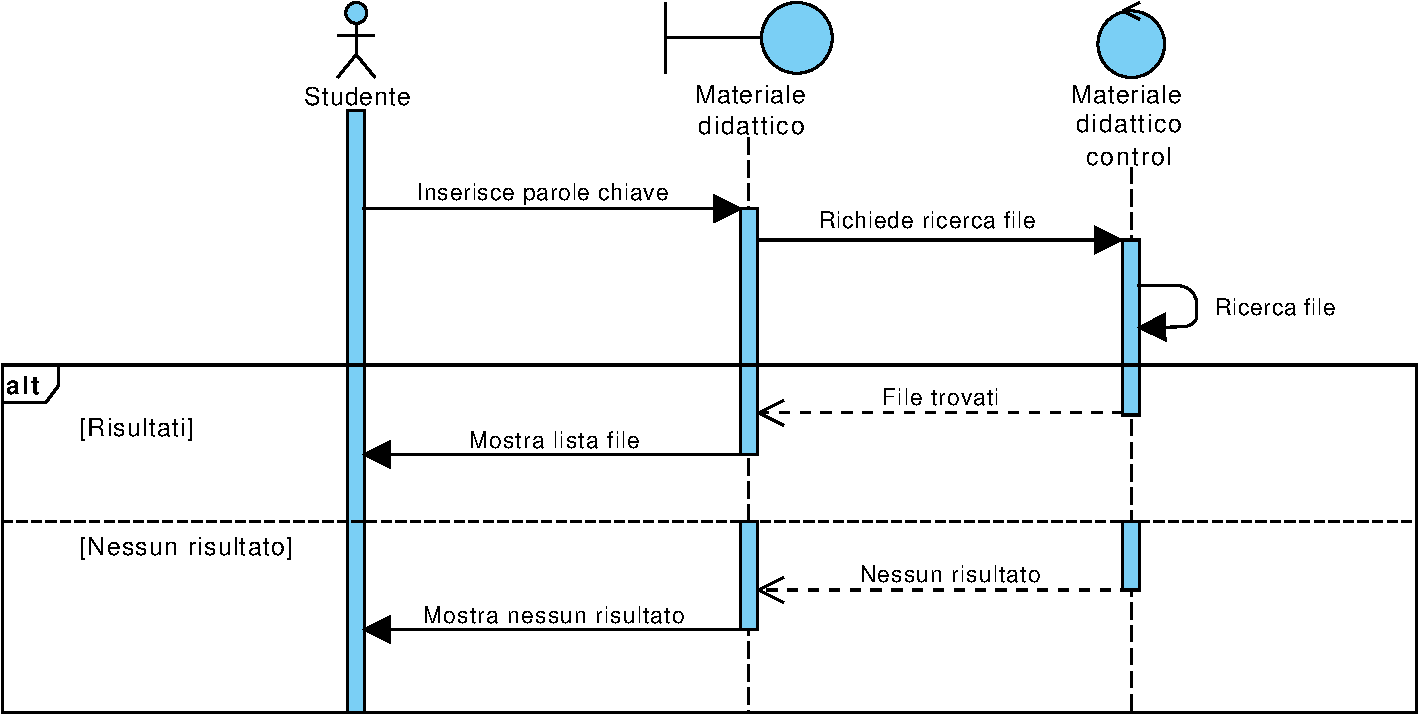
\includegraphics[width=6.5in]{imgs/gruppo1/sequence_diagrams/SD14_ricerca_file.pdf}
\end{center}
\newpage


%% 8.5.15 - Visualizza dettagli file %%
\subsection{Visualizza dettagli file}
\begin{center}
	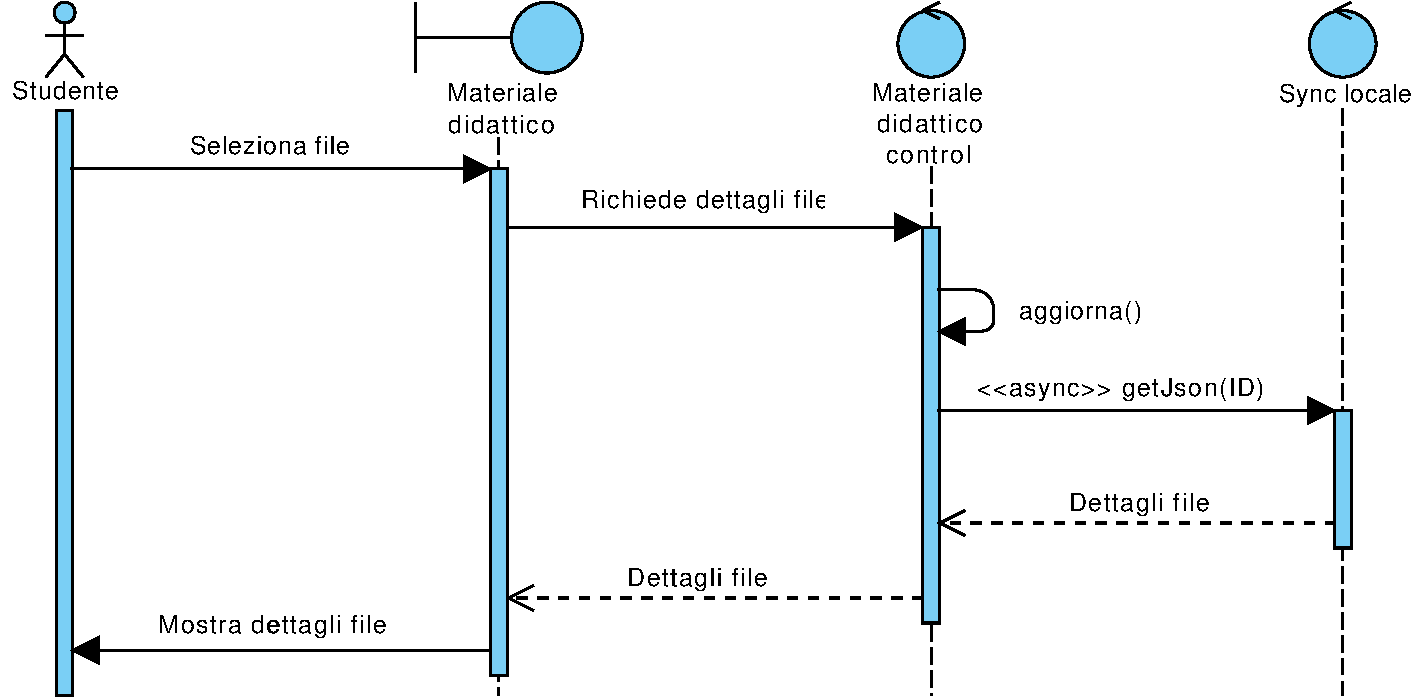
\includegraphics[width=6.5in]{imgs/gruppo1//sequence_diagrams/SD15_visualizza_dettagli_file.pdf}
\end{center}
%% 8.5.16- Apri file  %%
\subsection{Apri file}
\begin{center}
	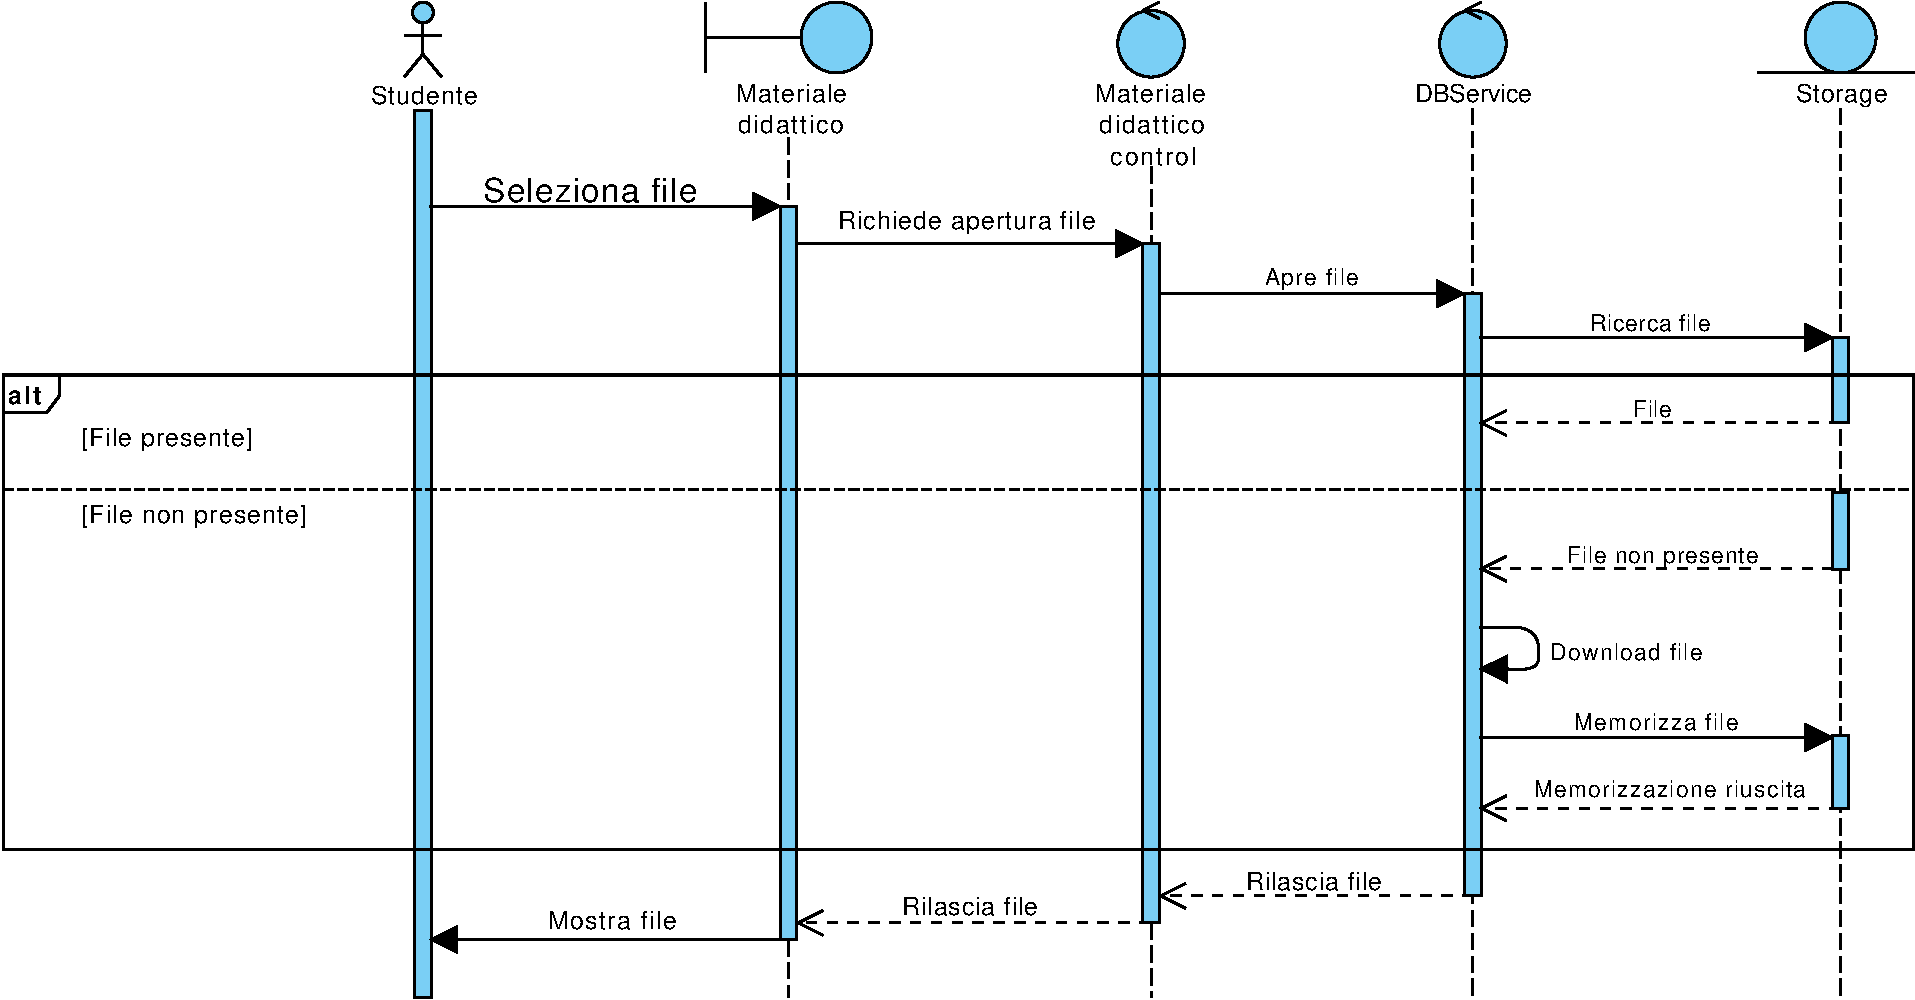
\includegraphics[width=6.5in]{imgs/gruppo1/sequence_diagrams/SD16_apri_file.pdf}
\end{center}
\newpage


%% 8.5.17 - Rimuovi file %%
\subsection{Rimuovi  file}
\begin{center}
	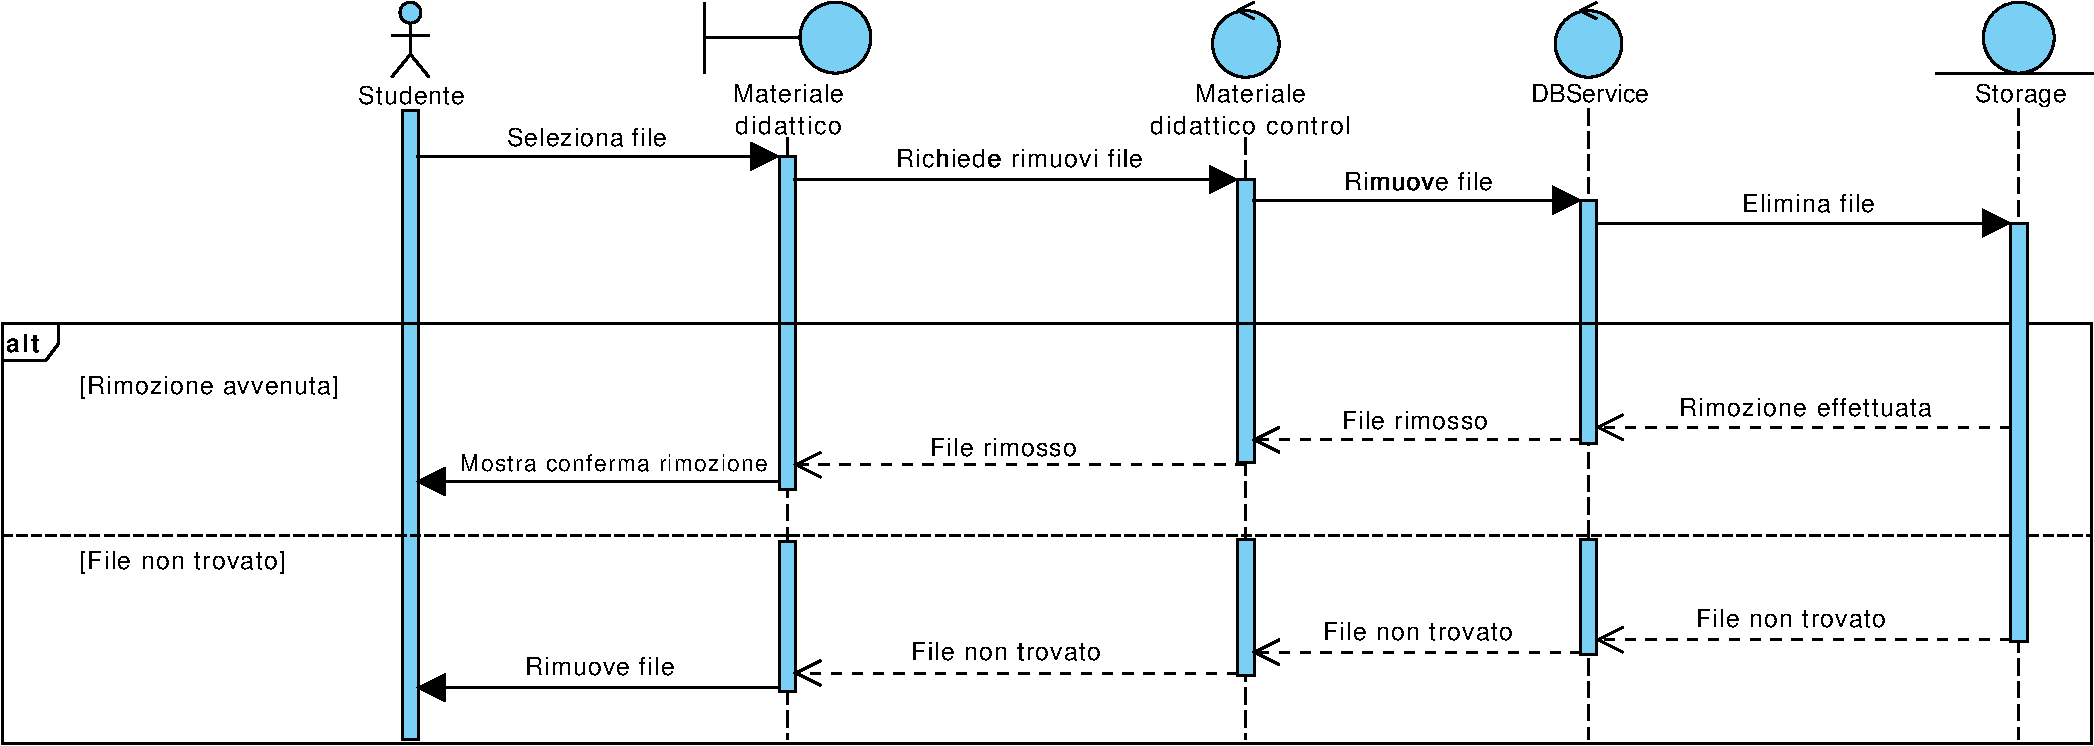
\includegraphics[width=6.5in]{imgs/gruppo1/sequence_diagrams/SD17_rimuovi_file.pdf}
\end{center}
\newpage




\section{Diagrammi delle attività}

%% 8.6.1 - Visualizza corsi %%
\subsection{Visualizza corsi}
\begin{center}
	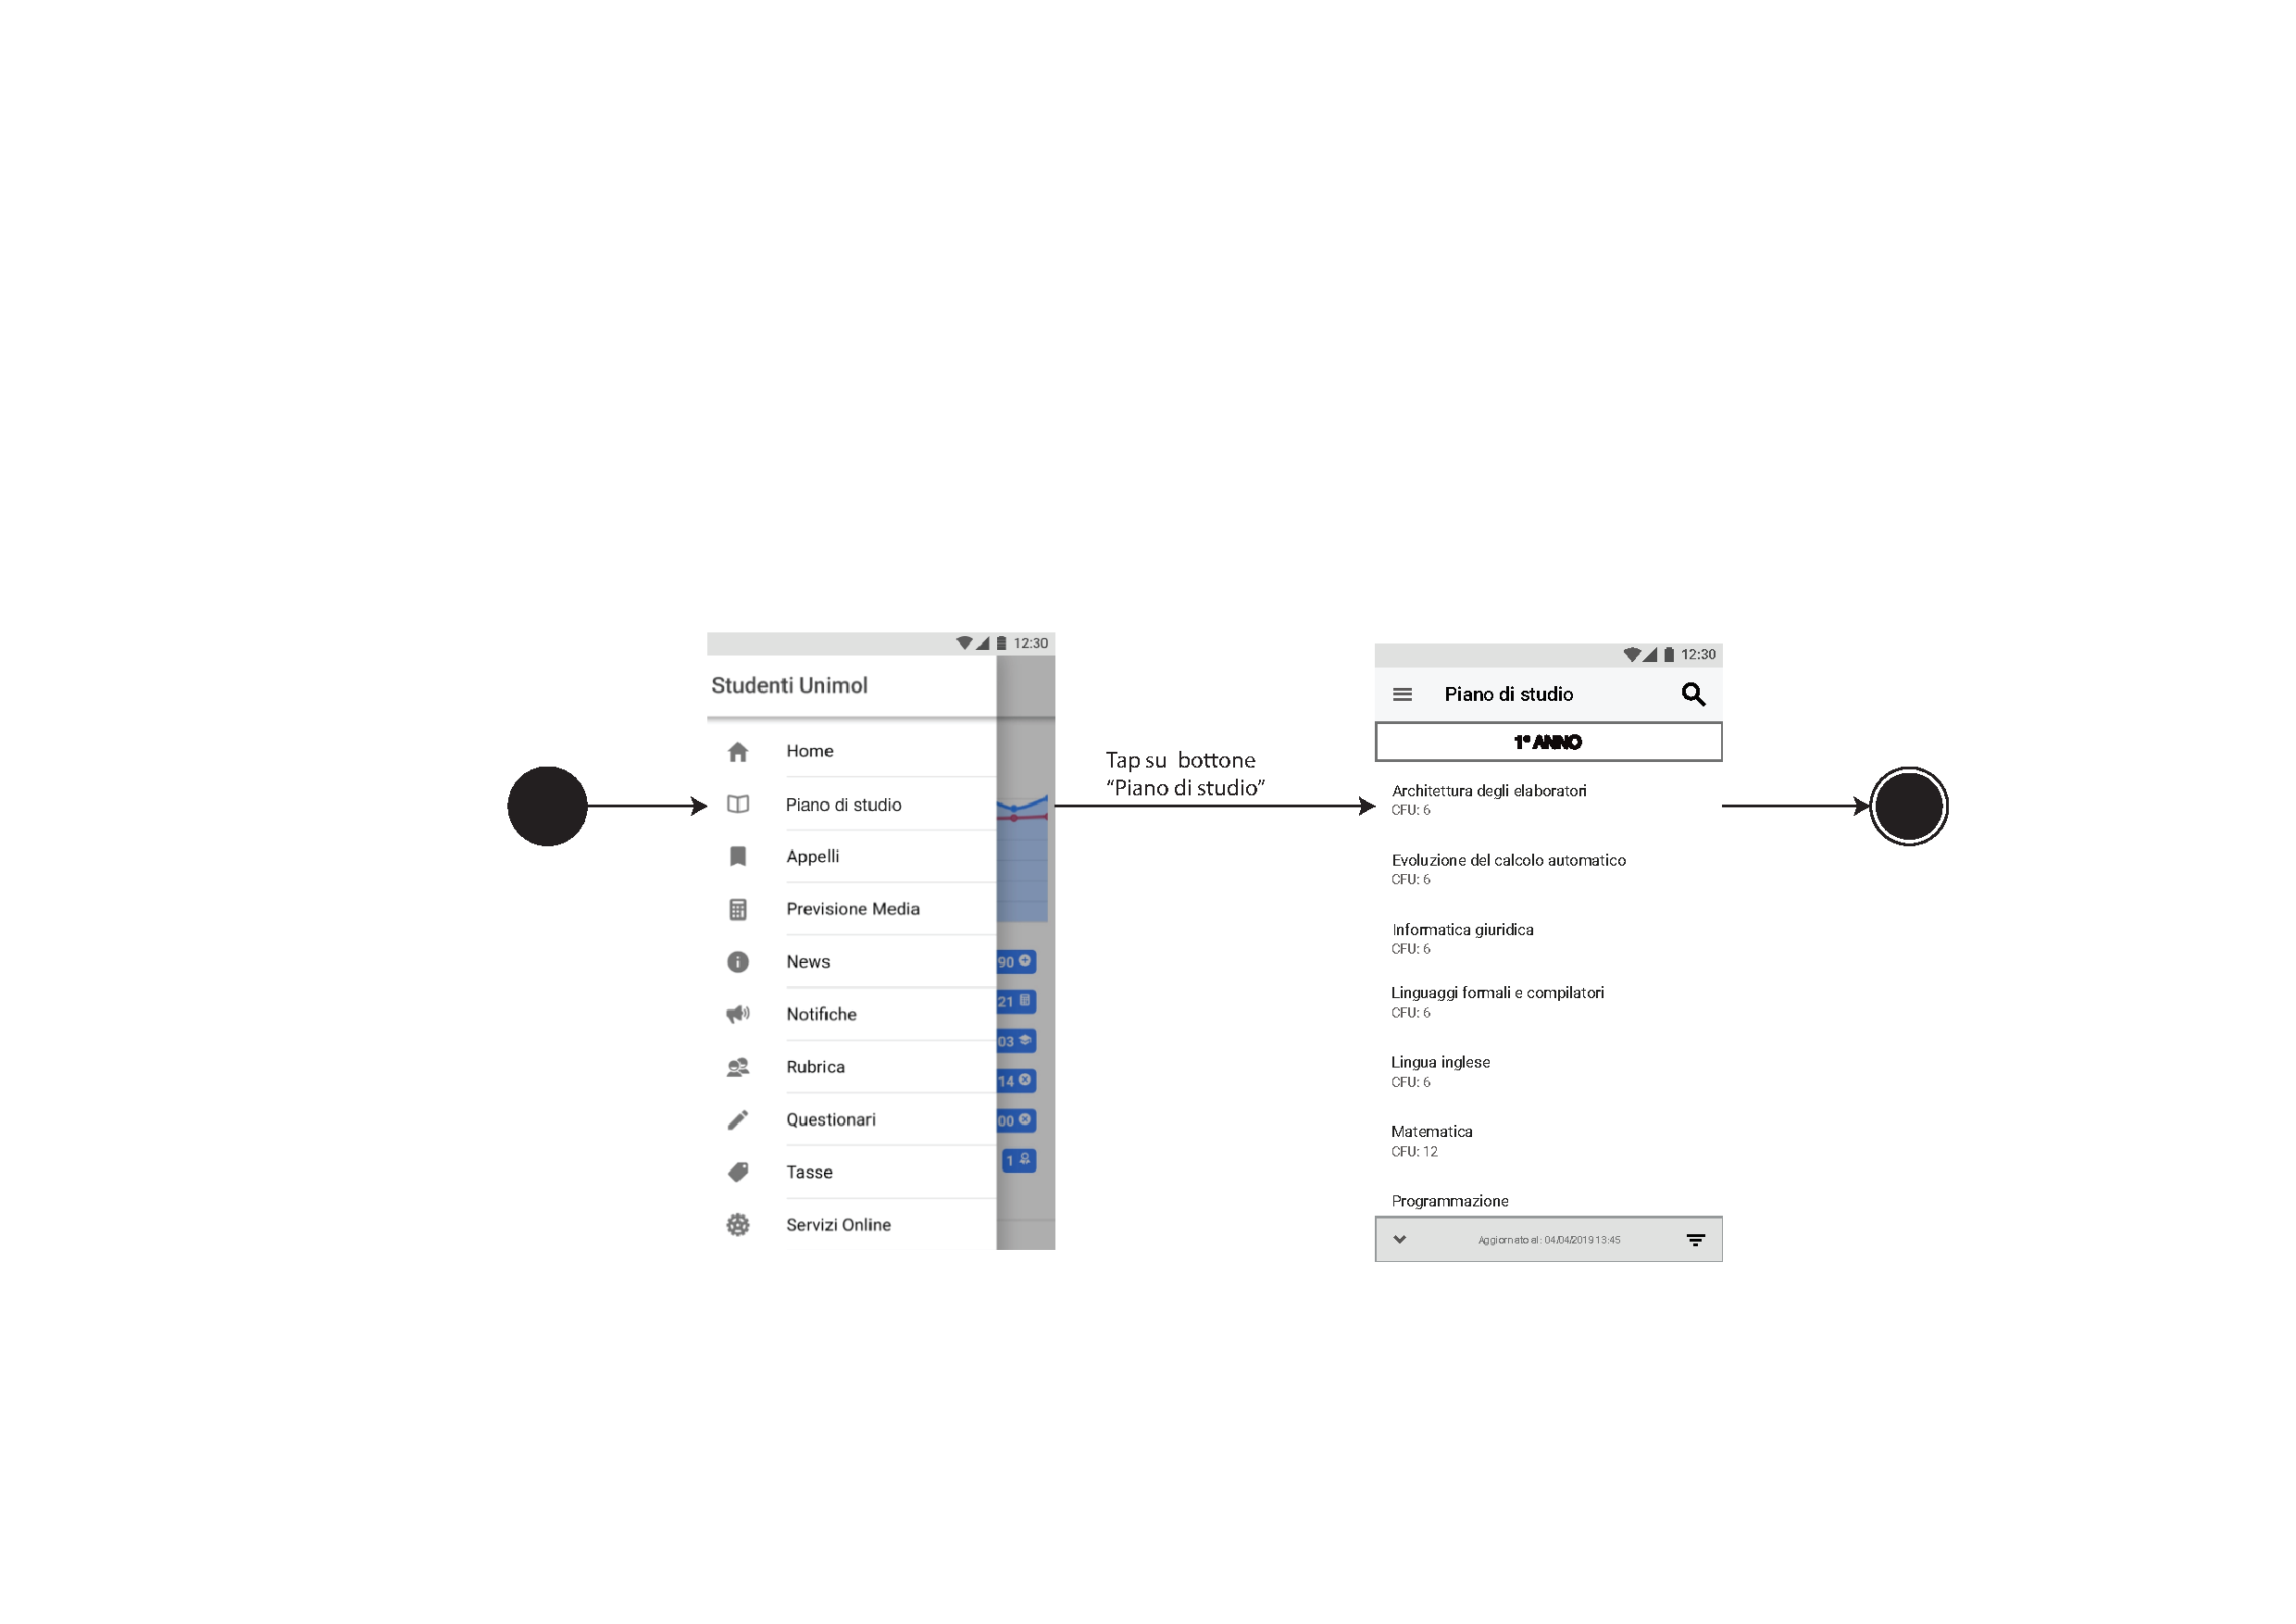
\includegraphics[width=6in]{imgs/gruppo1/activity_diagrams/AD1_Visualizza_corsi.pdf}
\end{center}
\newpage

%%8.6.2 - Ricerca corsi  %%

\subsection{Ricerca corsi }
\begin{center}
	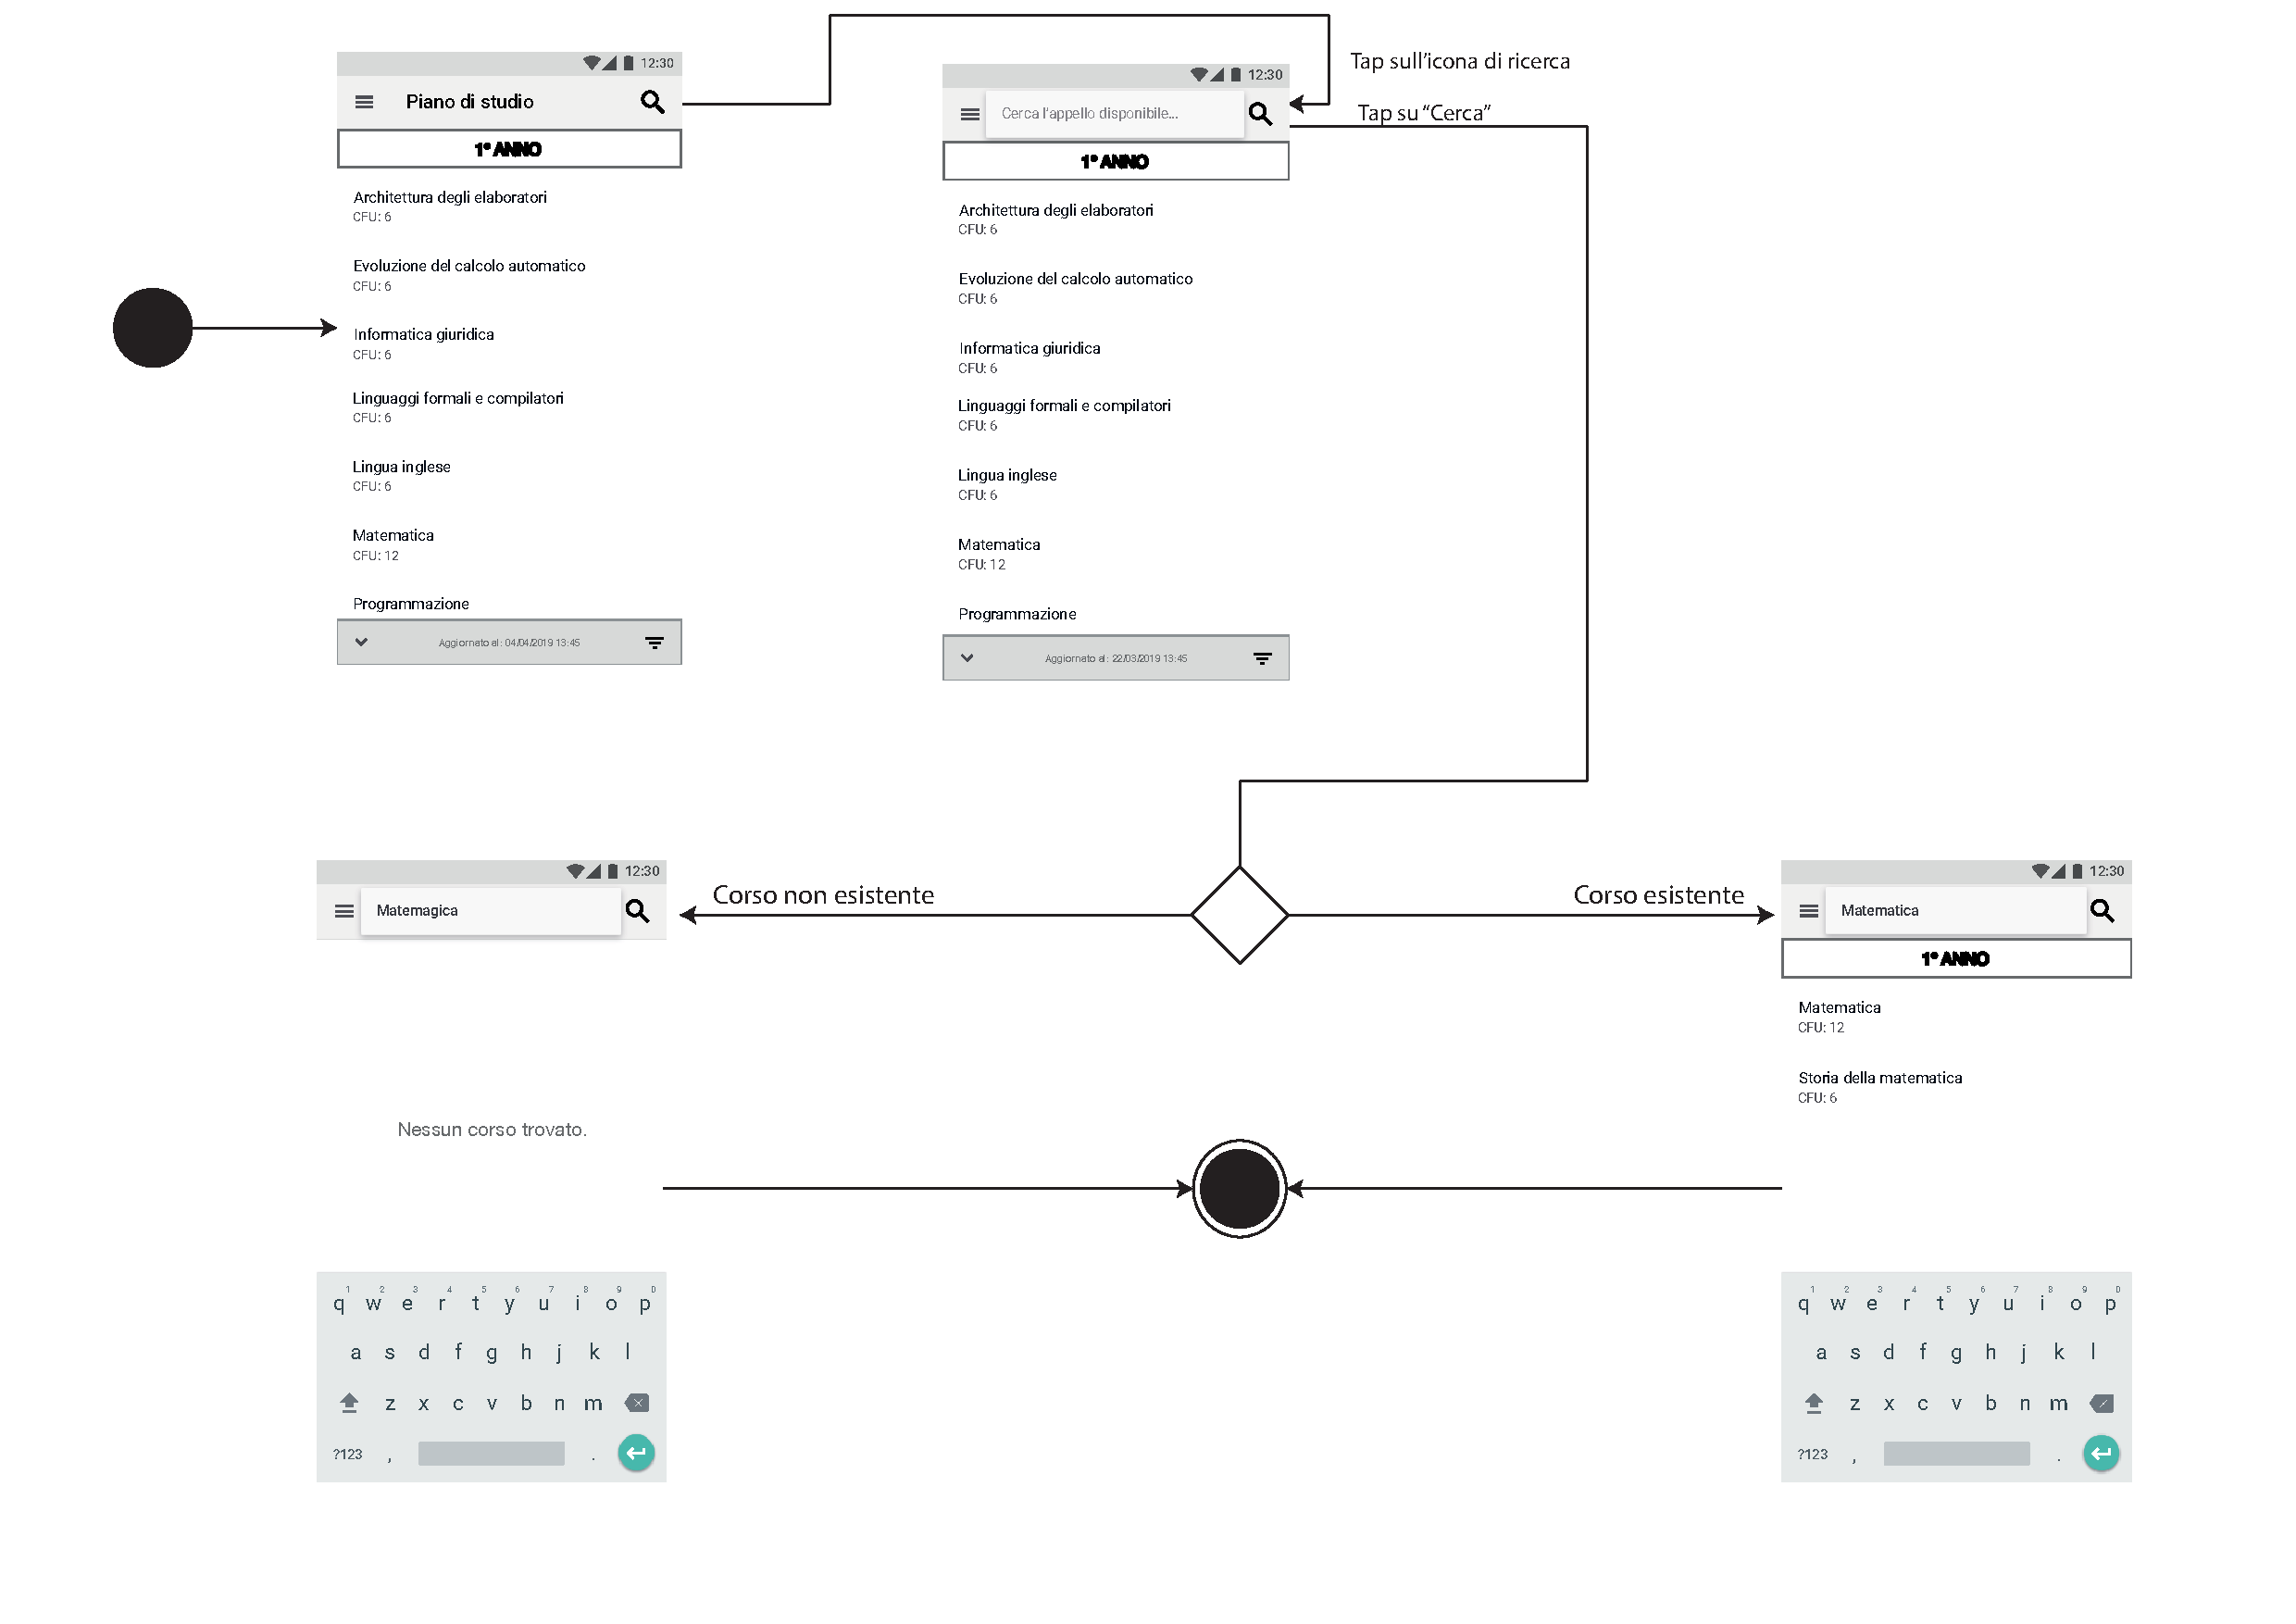
\includegraphics[width=6in]{imgs/gruppo1/activity_diagrams/AD2_ricerca_corsi.pdf}
\end{center}
\newpage

%%8.6.3 - Filtra corsi con memorizzazione %%

\subsection{Filtra corsi con memorizzazione  }
\begin{center}
	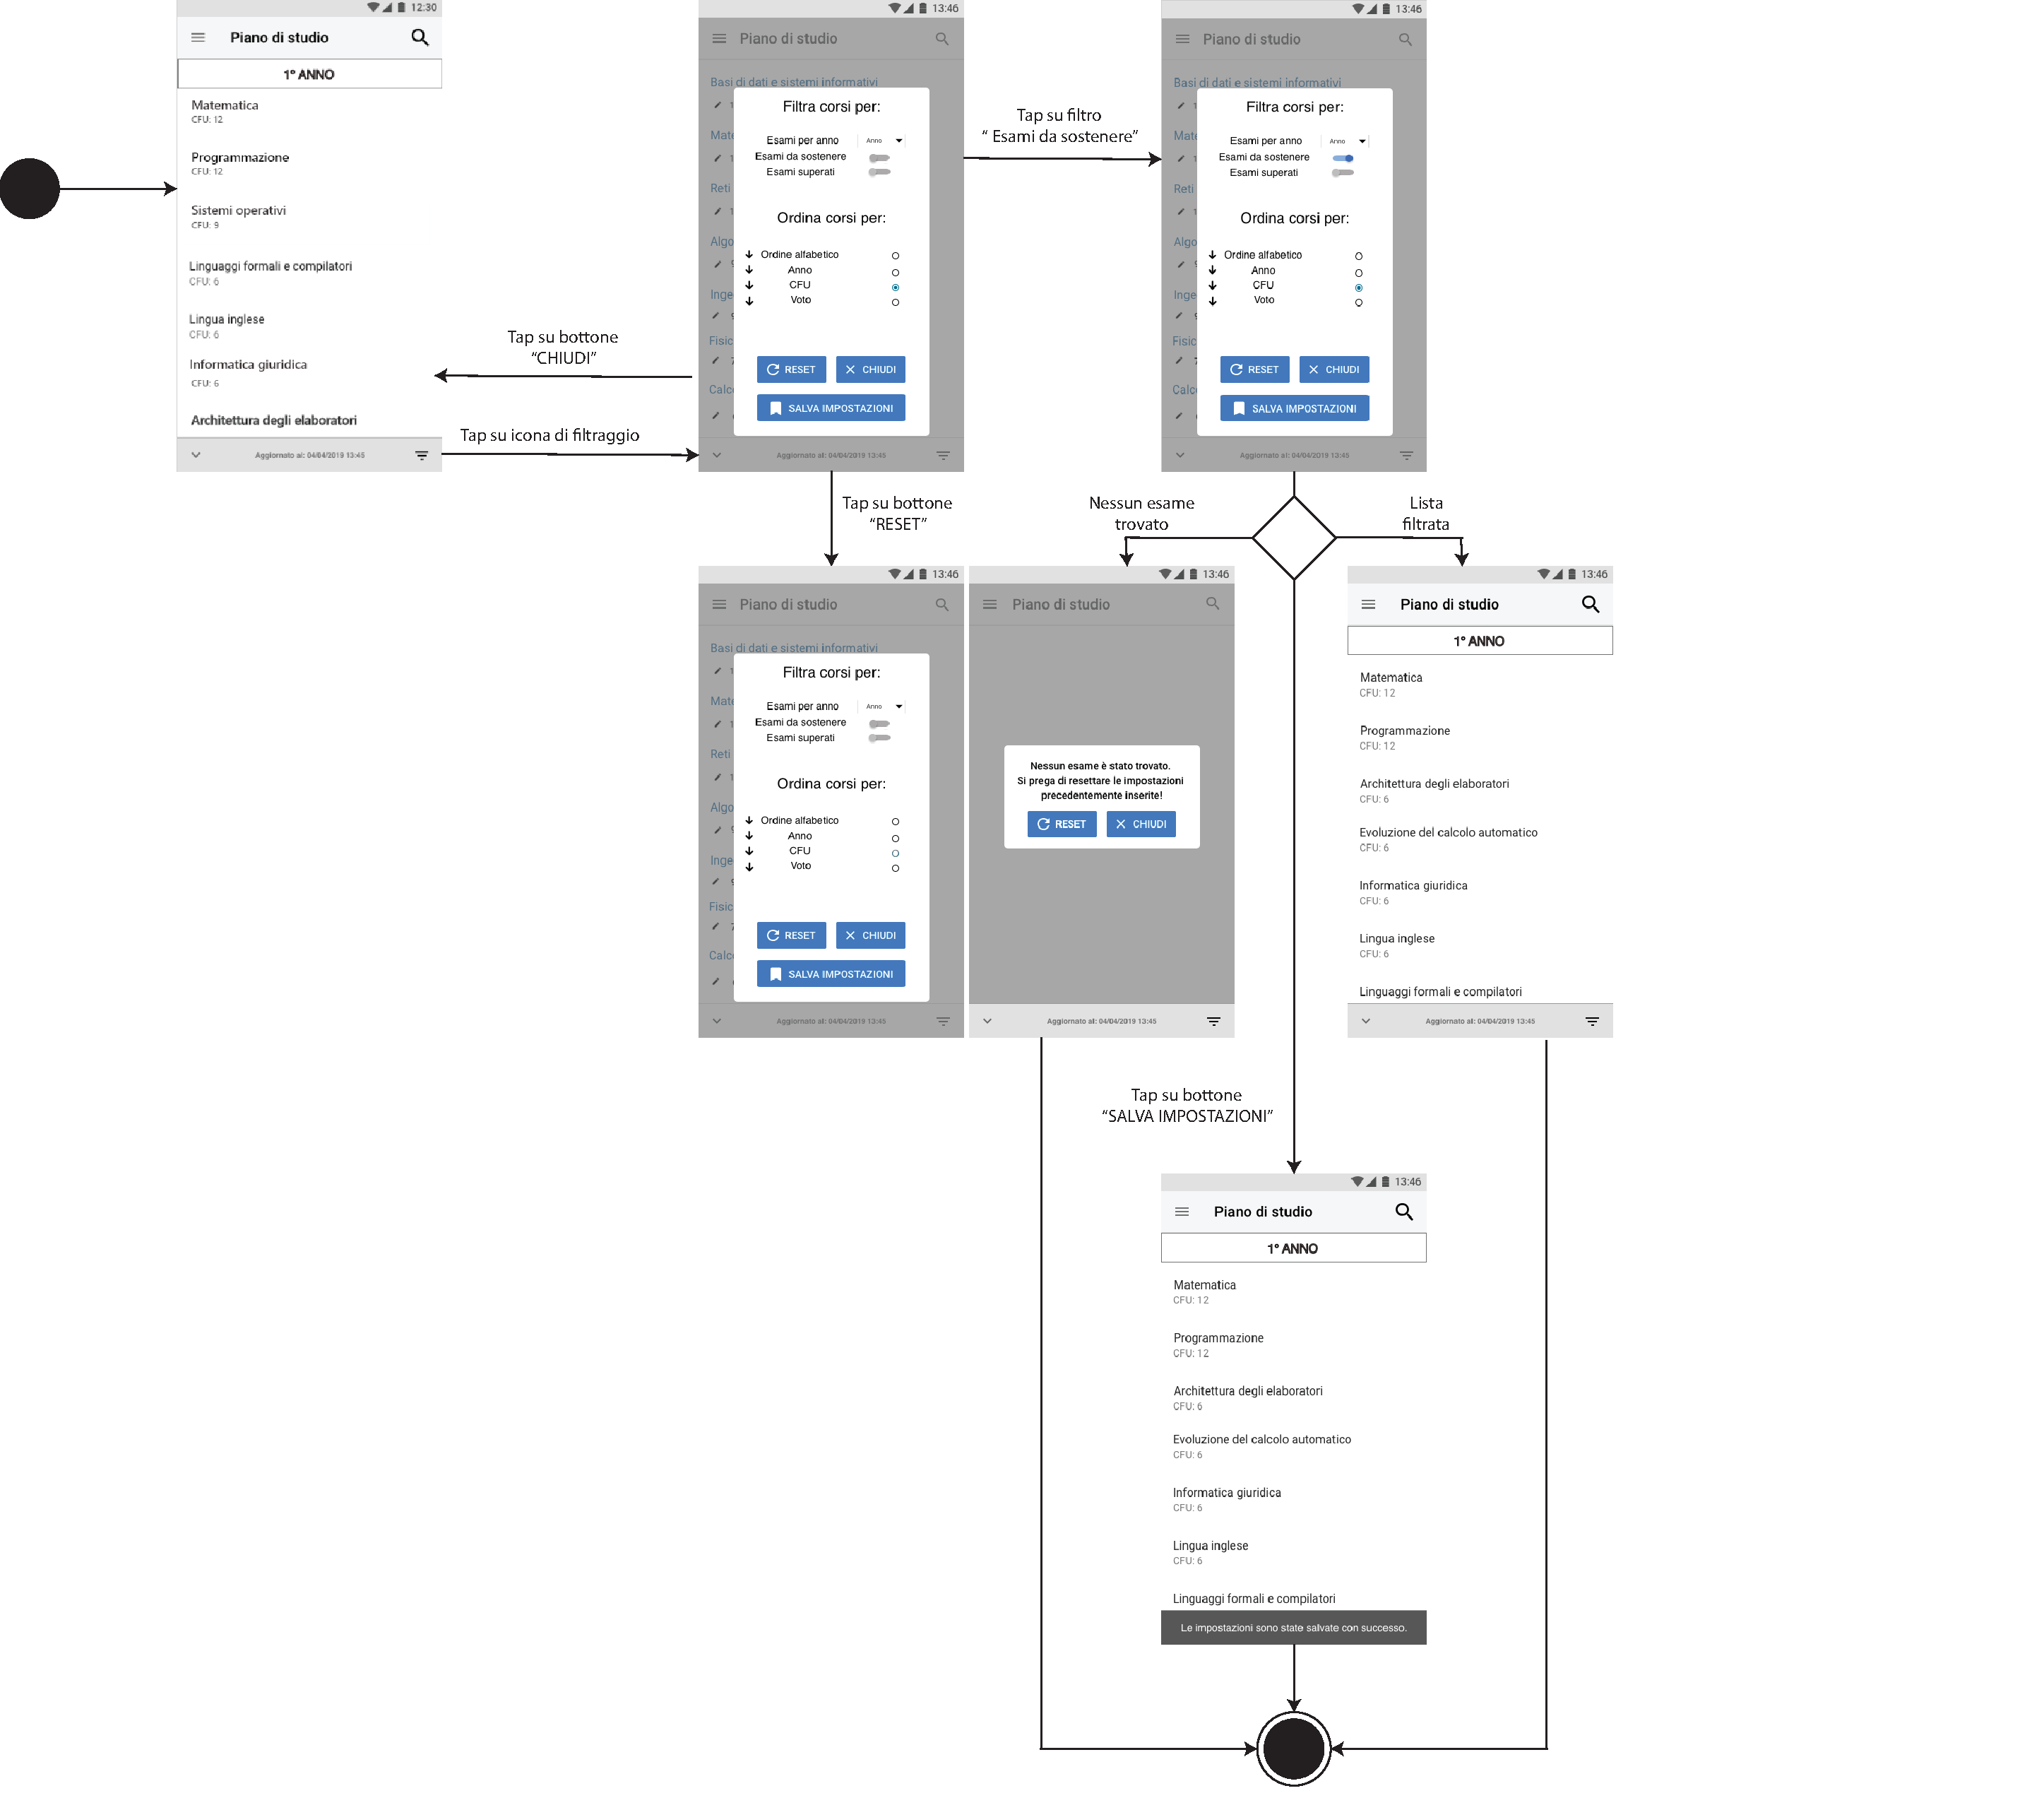
\includegraphics[width=6in]{imgs/gruppo1/activity_diagrams/AD3_filtra_corsi.pdf}
\end{center}
\newpage

%%8.6.4 - Ordina corsi con memorizzazione %%

\subsection{Ordina corsi con memorizzazione}
\begin{center}
	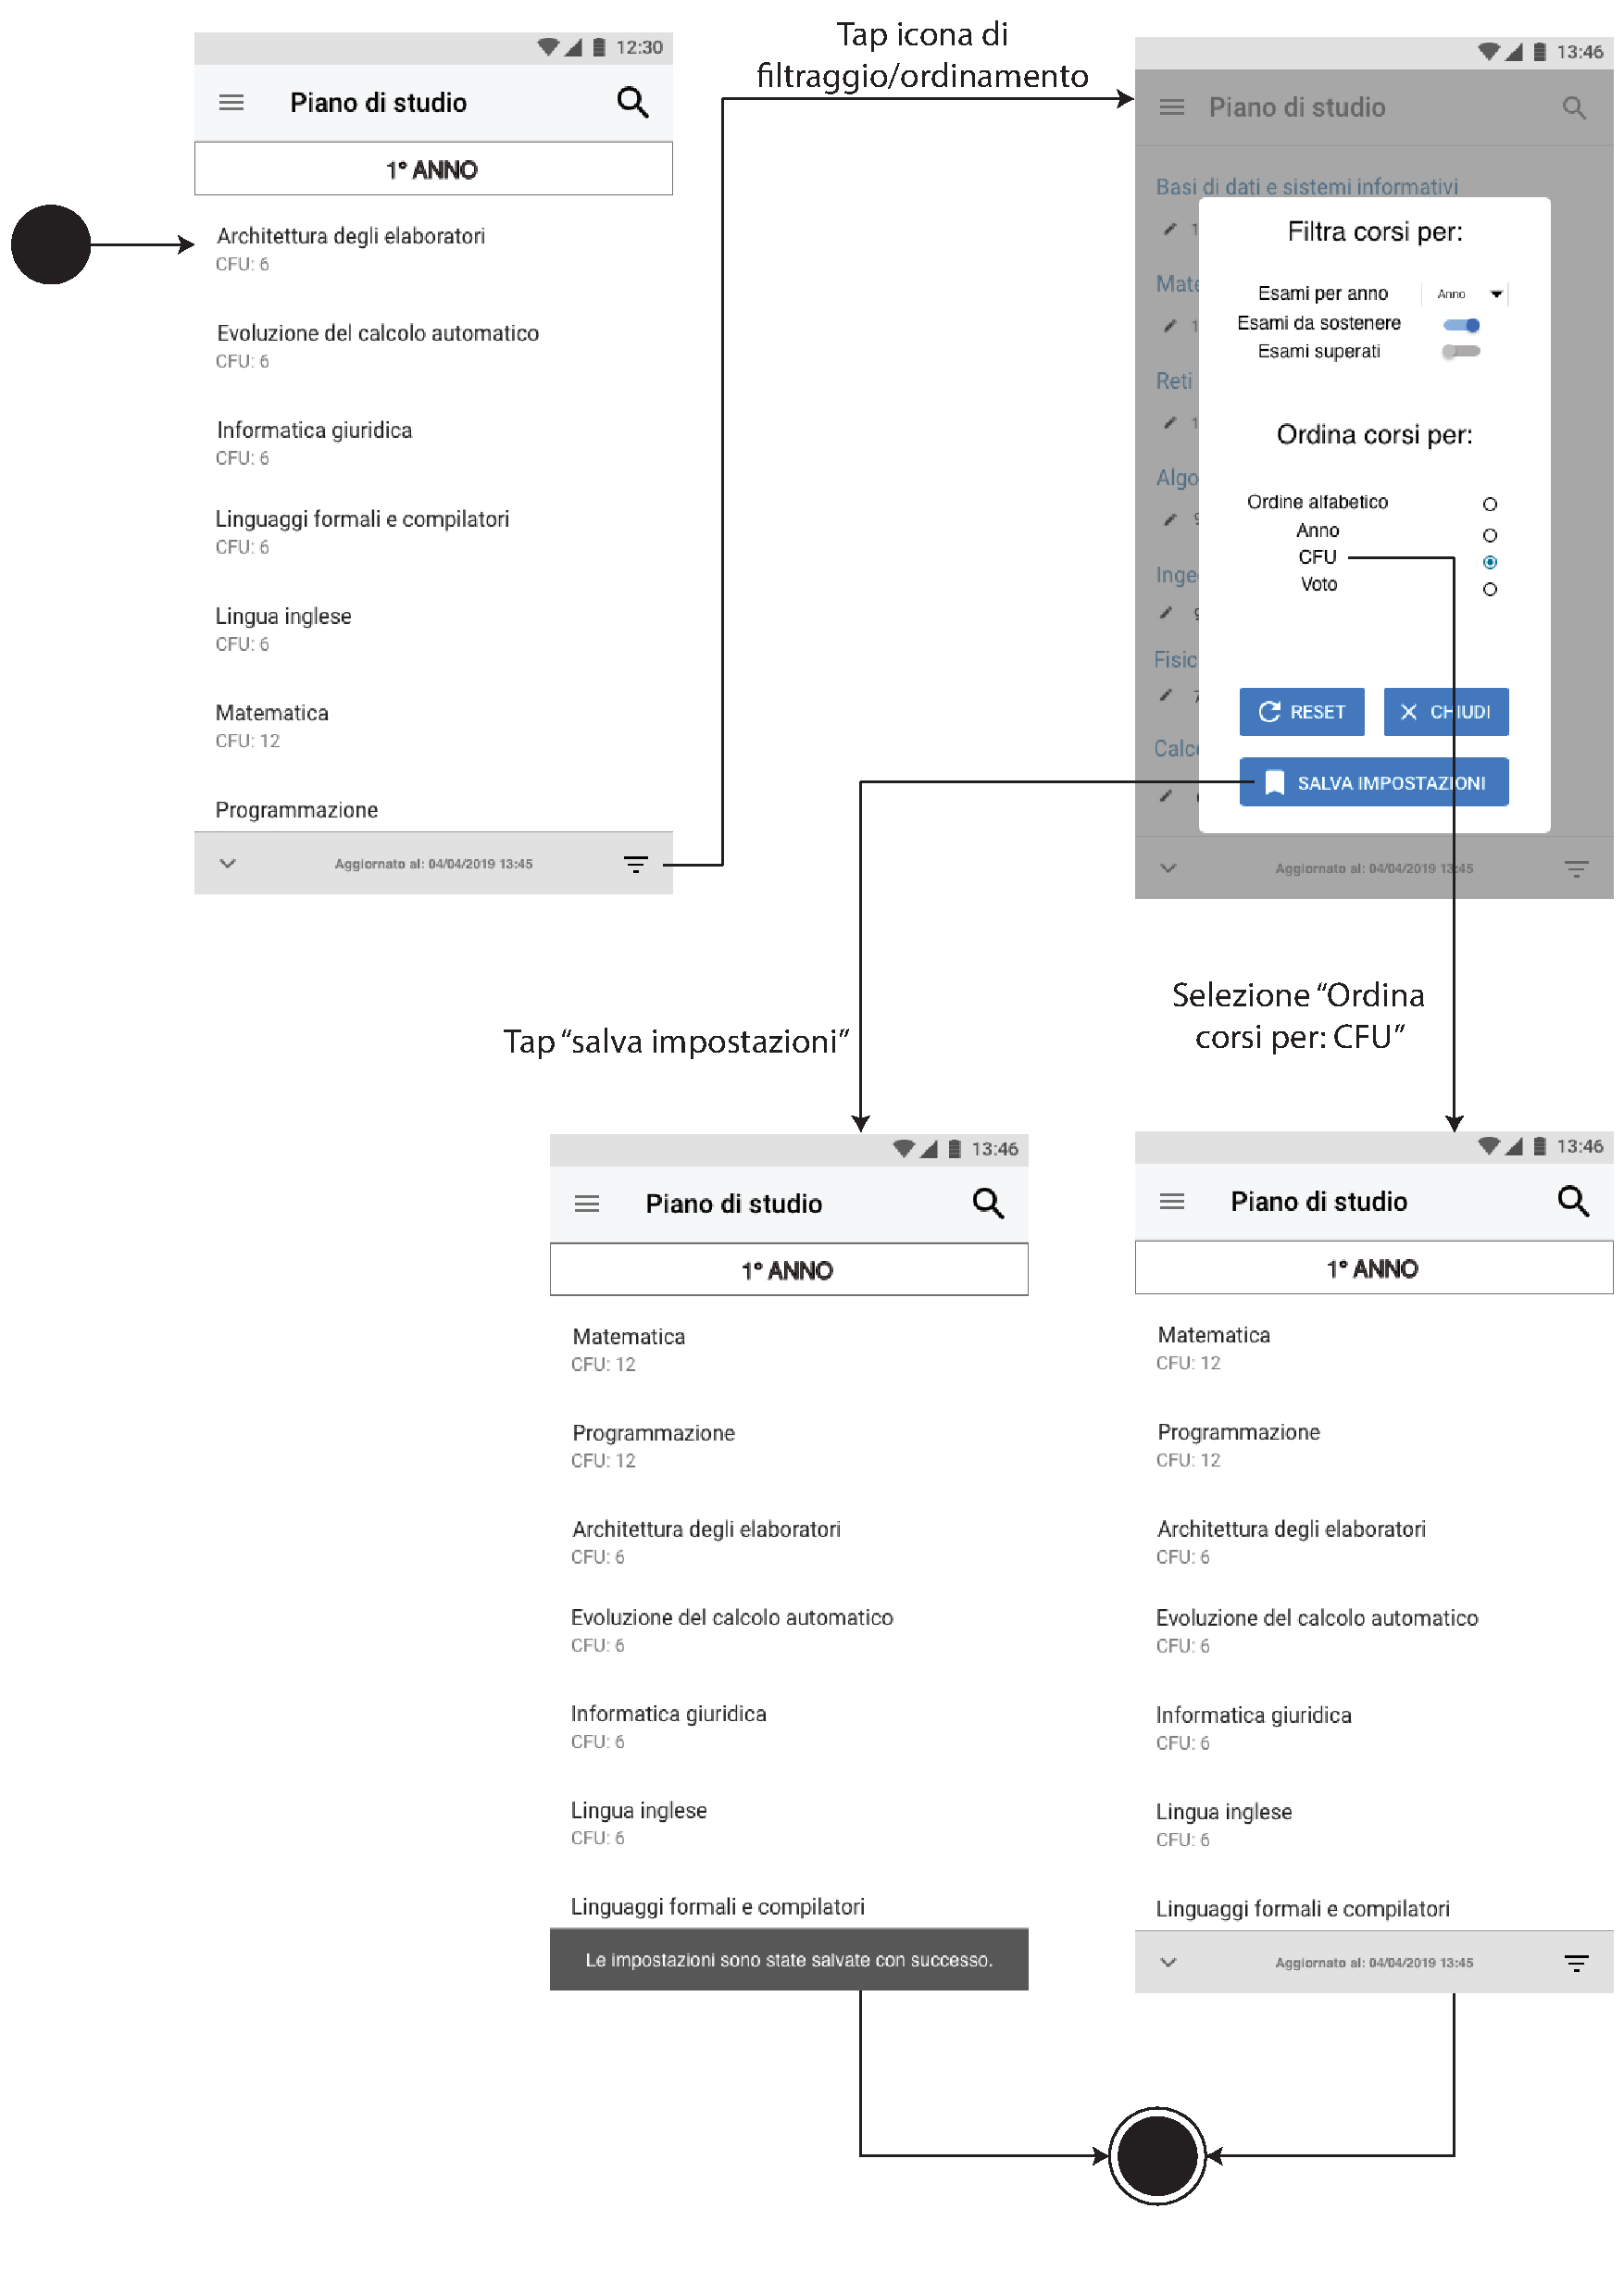
\includegraphics[width=6in]{imgs/gruppo1/activity_diagrams/AD4_ordina_corsi.pdf}
\end{center}
\newpage

%%8.6.5 - Visualizza dettagli corso%%

\subsection{Visualizza dettagli corso}
\begin{center}
	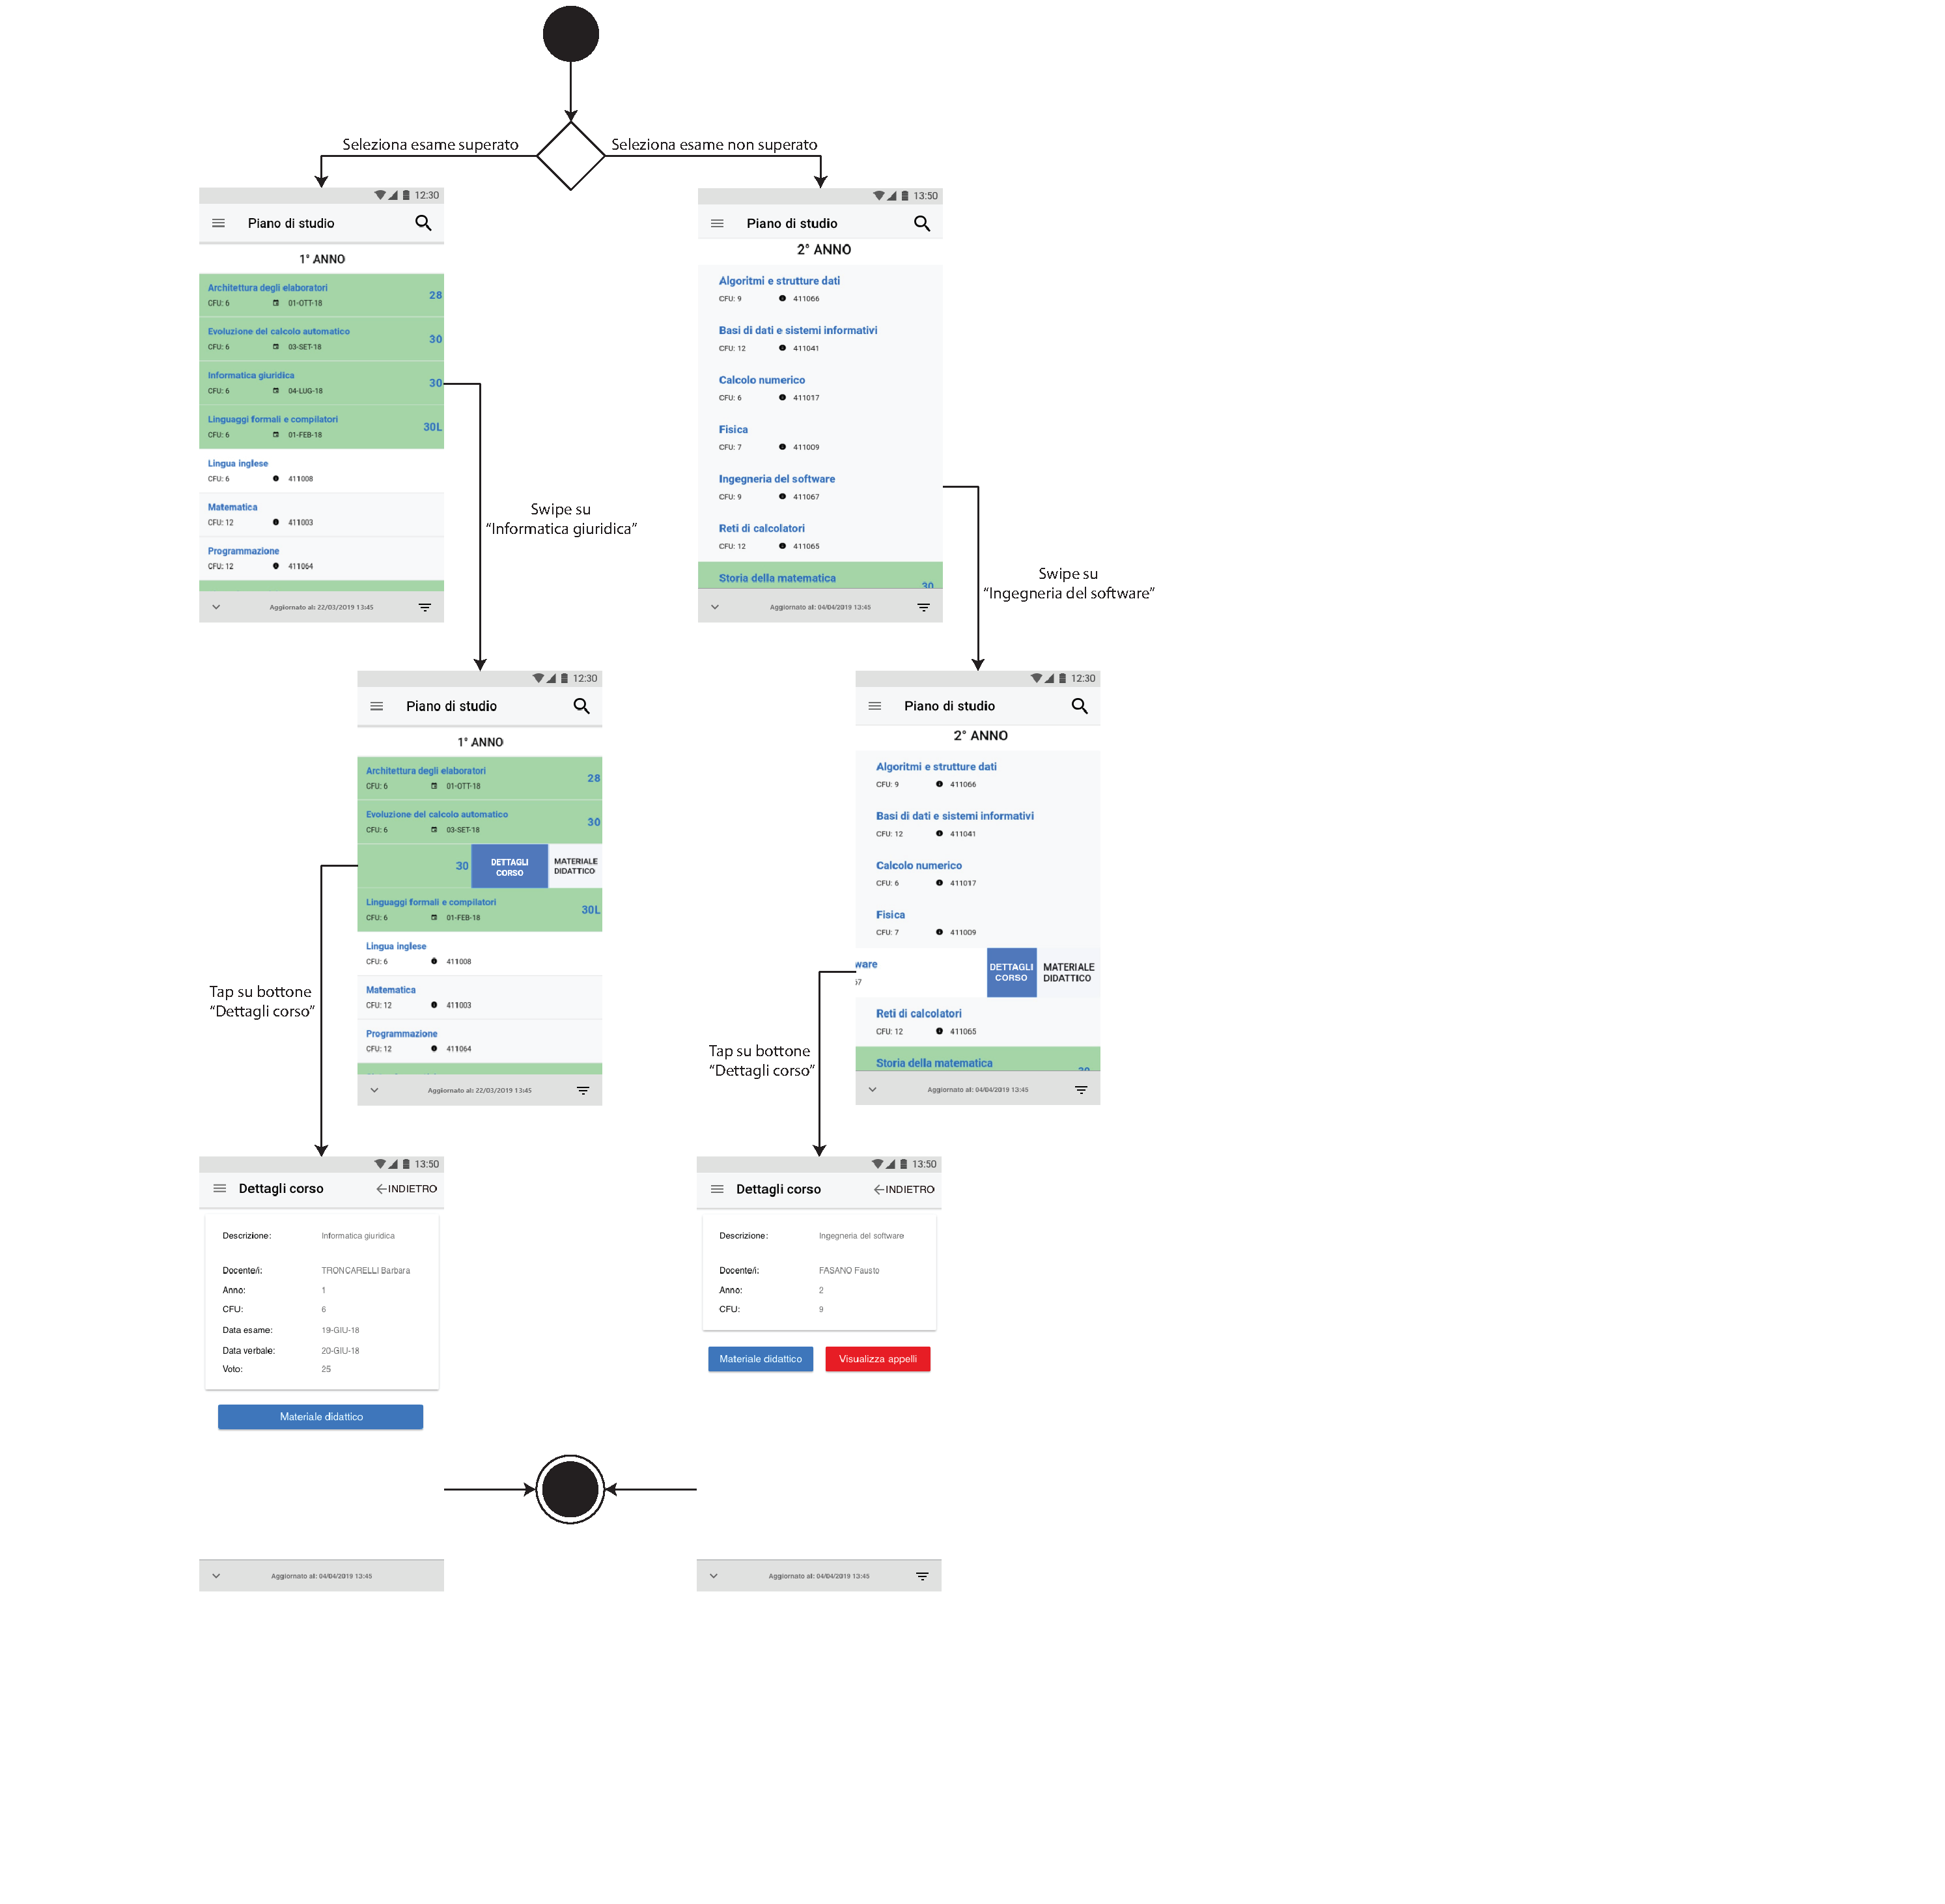
\includegraphics[width=7in]{imgs/gruppo1/activity_diagrams/AD5_visualizza_dettagli_corso.pdf}
\end{center}
\newpage

%%8.6.6 - Visualizza appelli disponibili%%

\subsection{Visualizza appelli disponibil}
\begin{center}
	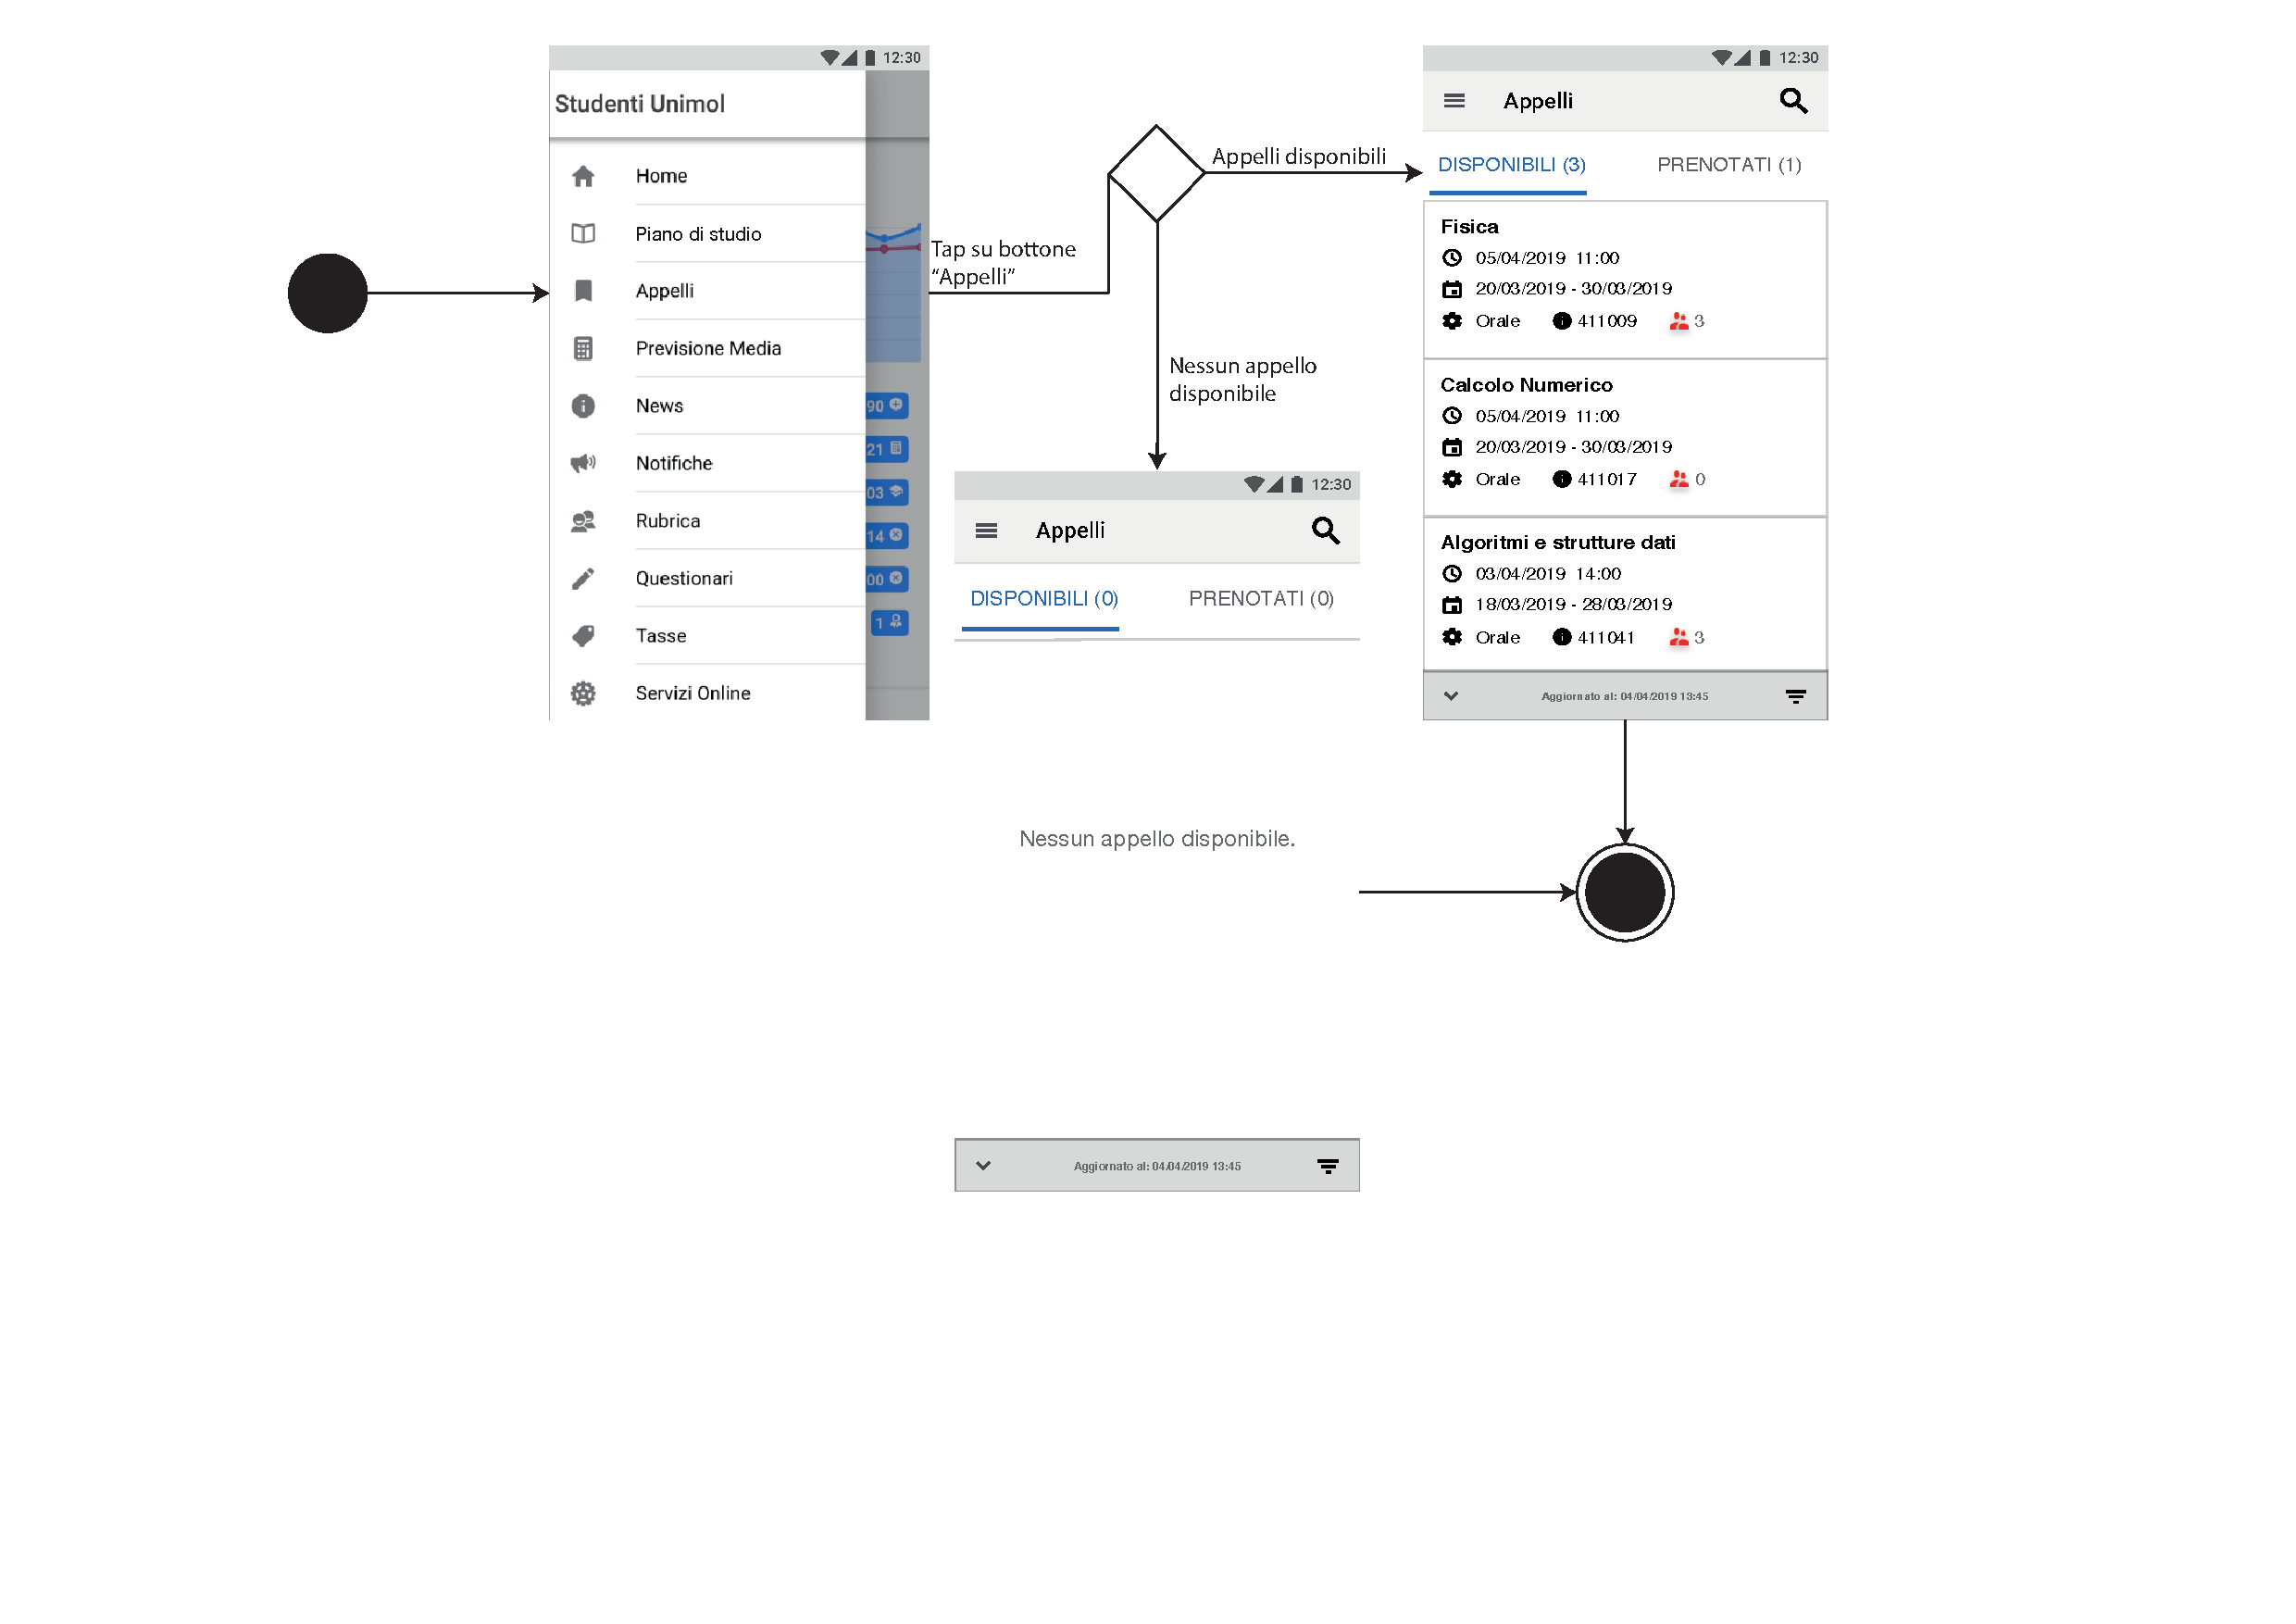
\includegraphics[width=6in]{imgs/gruppo1/activity_diagrams/AD6_visualizza_appelli_disponibili.pdf}
\end{center}
\newpage

%%8.6.7 - Visualizza appelli prenotati%%

\subsection{Visualizza appelli prenotati}
\begin{center}
	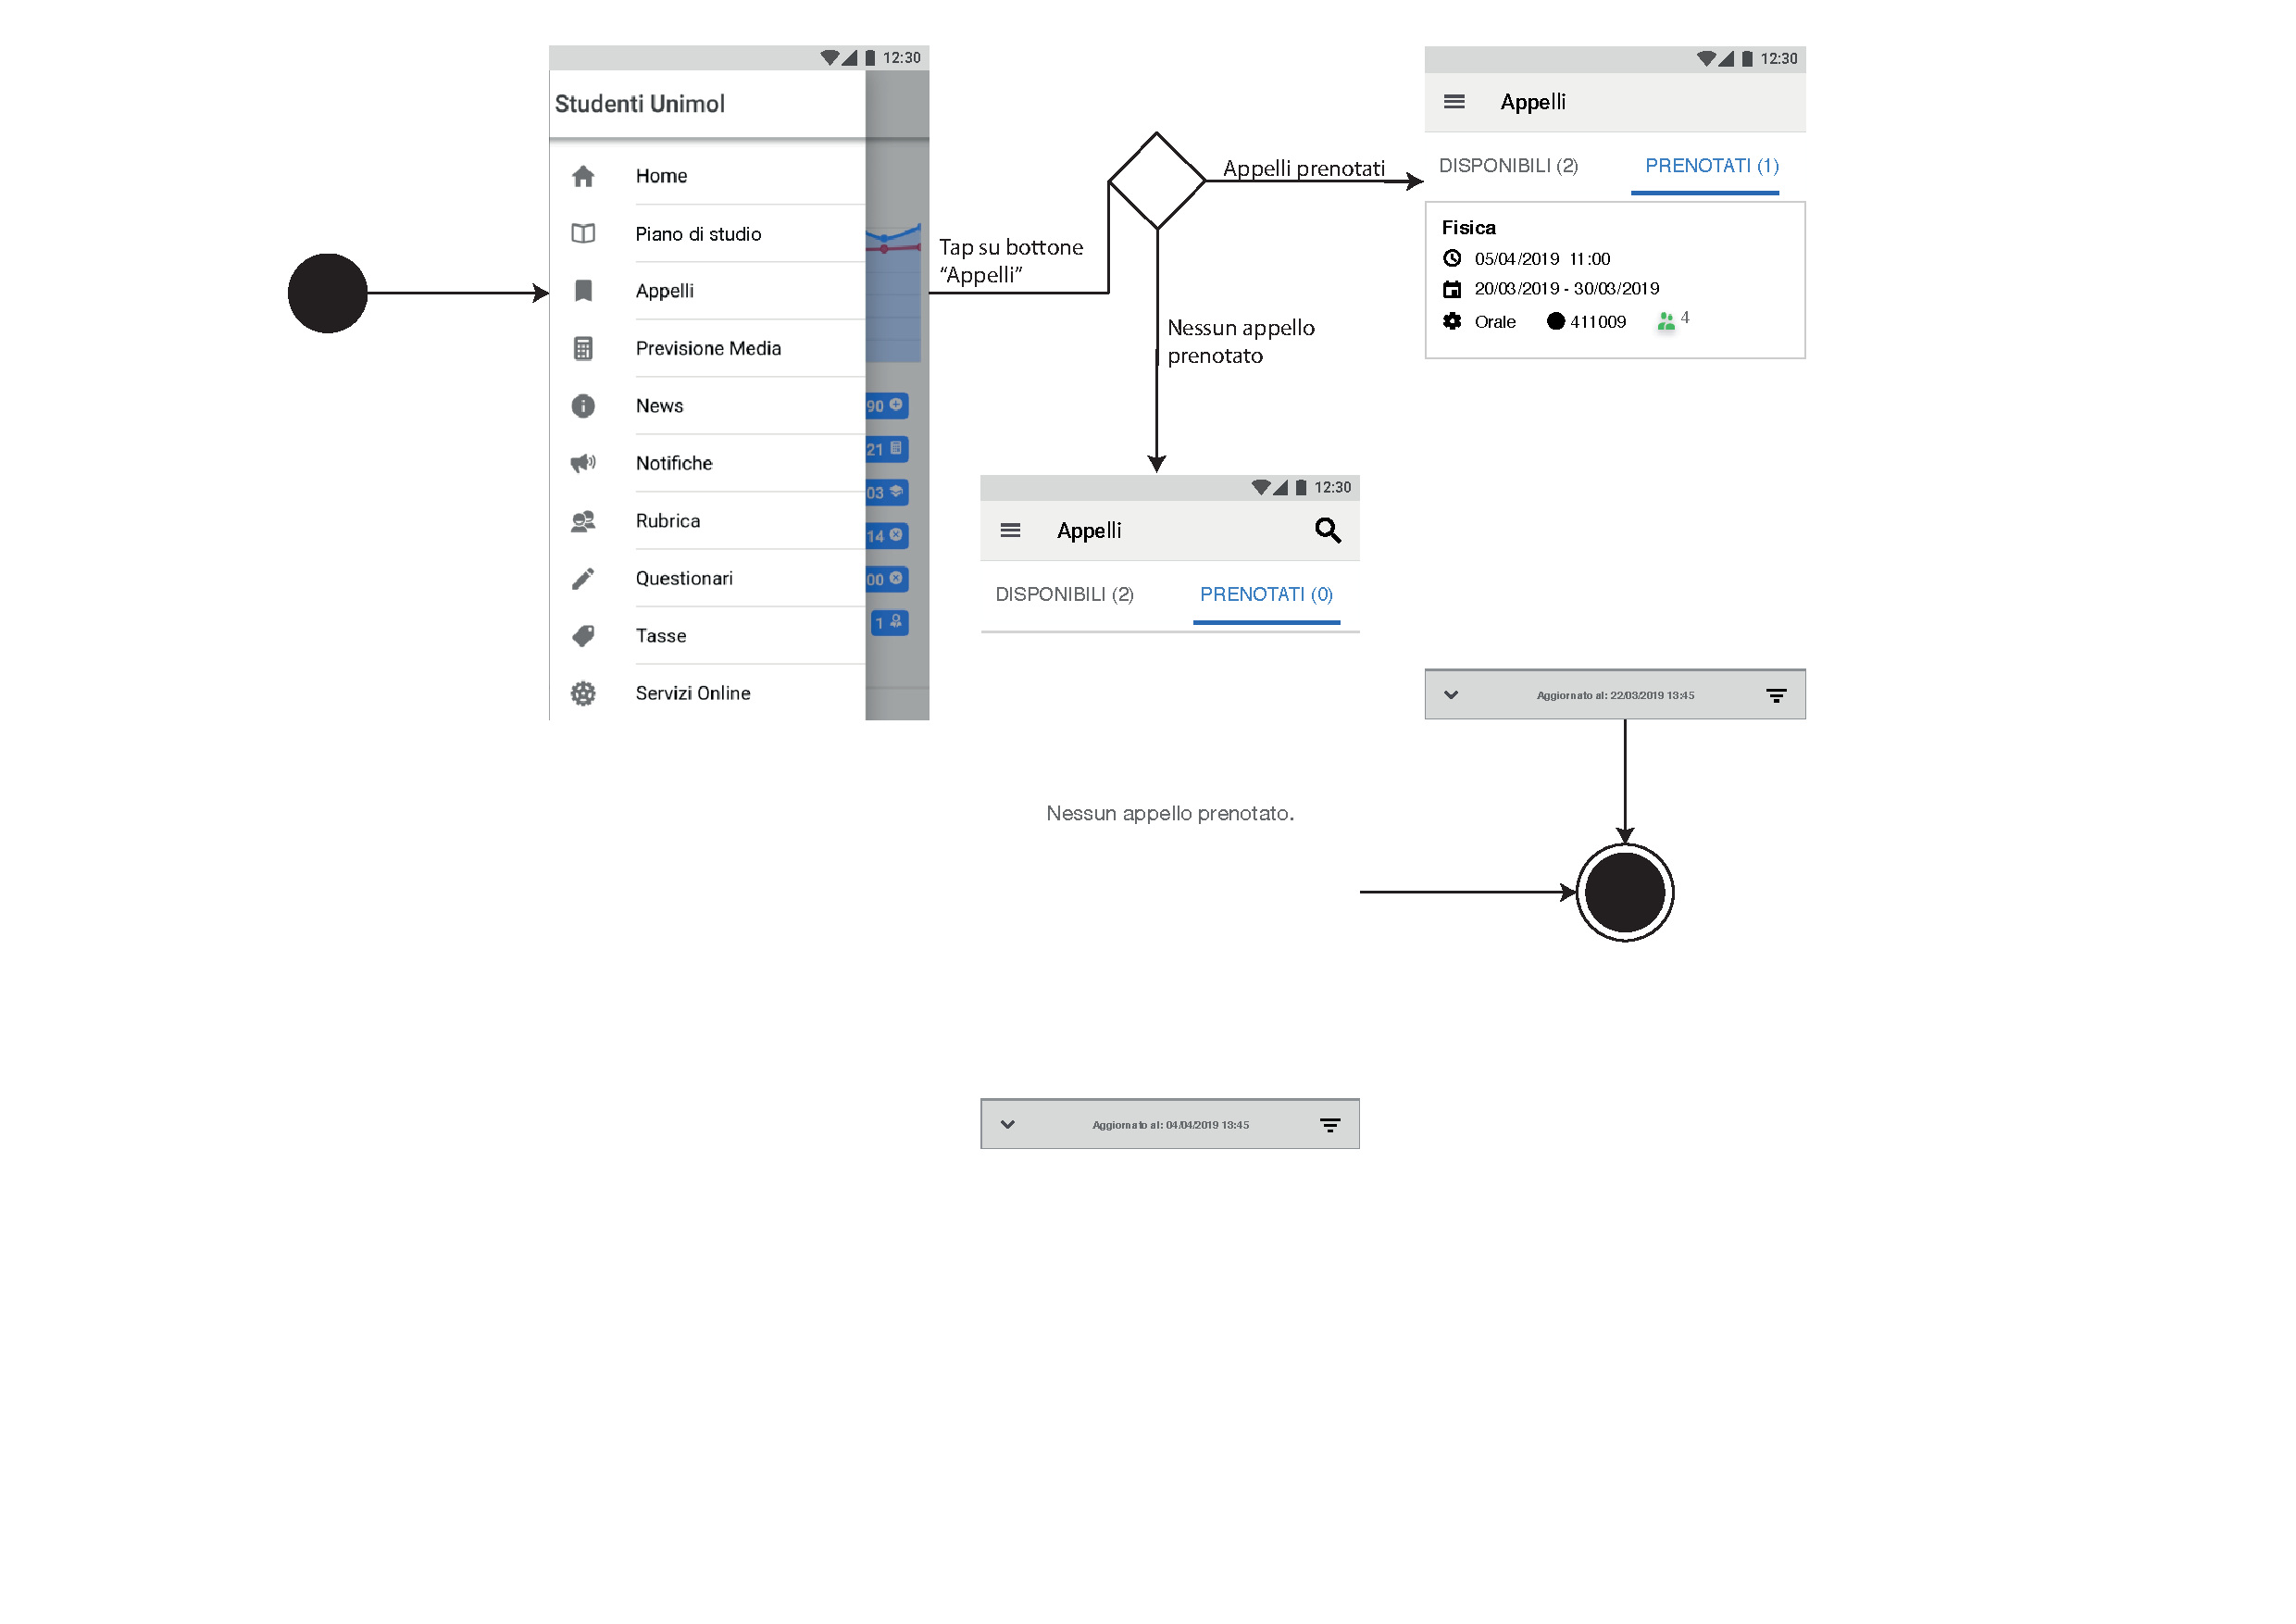
\includegraphics[width=6in]{imgs/gruppo1/activity_diagrams/AD7_visualizza_appelli_prenotati.pdf}
\end{center}
\newpage

%%8.6.8 - Ricerca appelli disponibili %%

\subsection{Ricerca appelli disponibili}
\begin{center}
	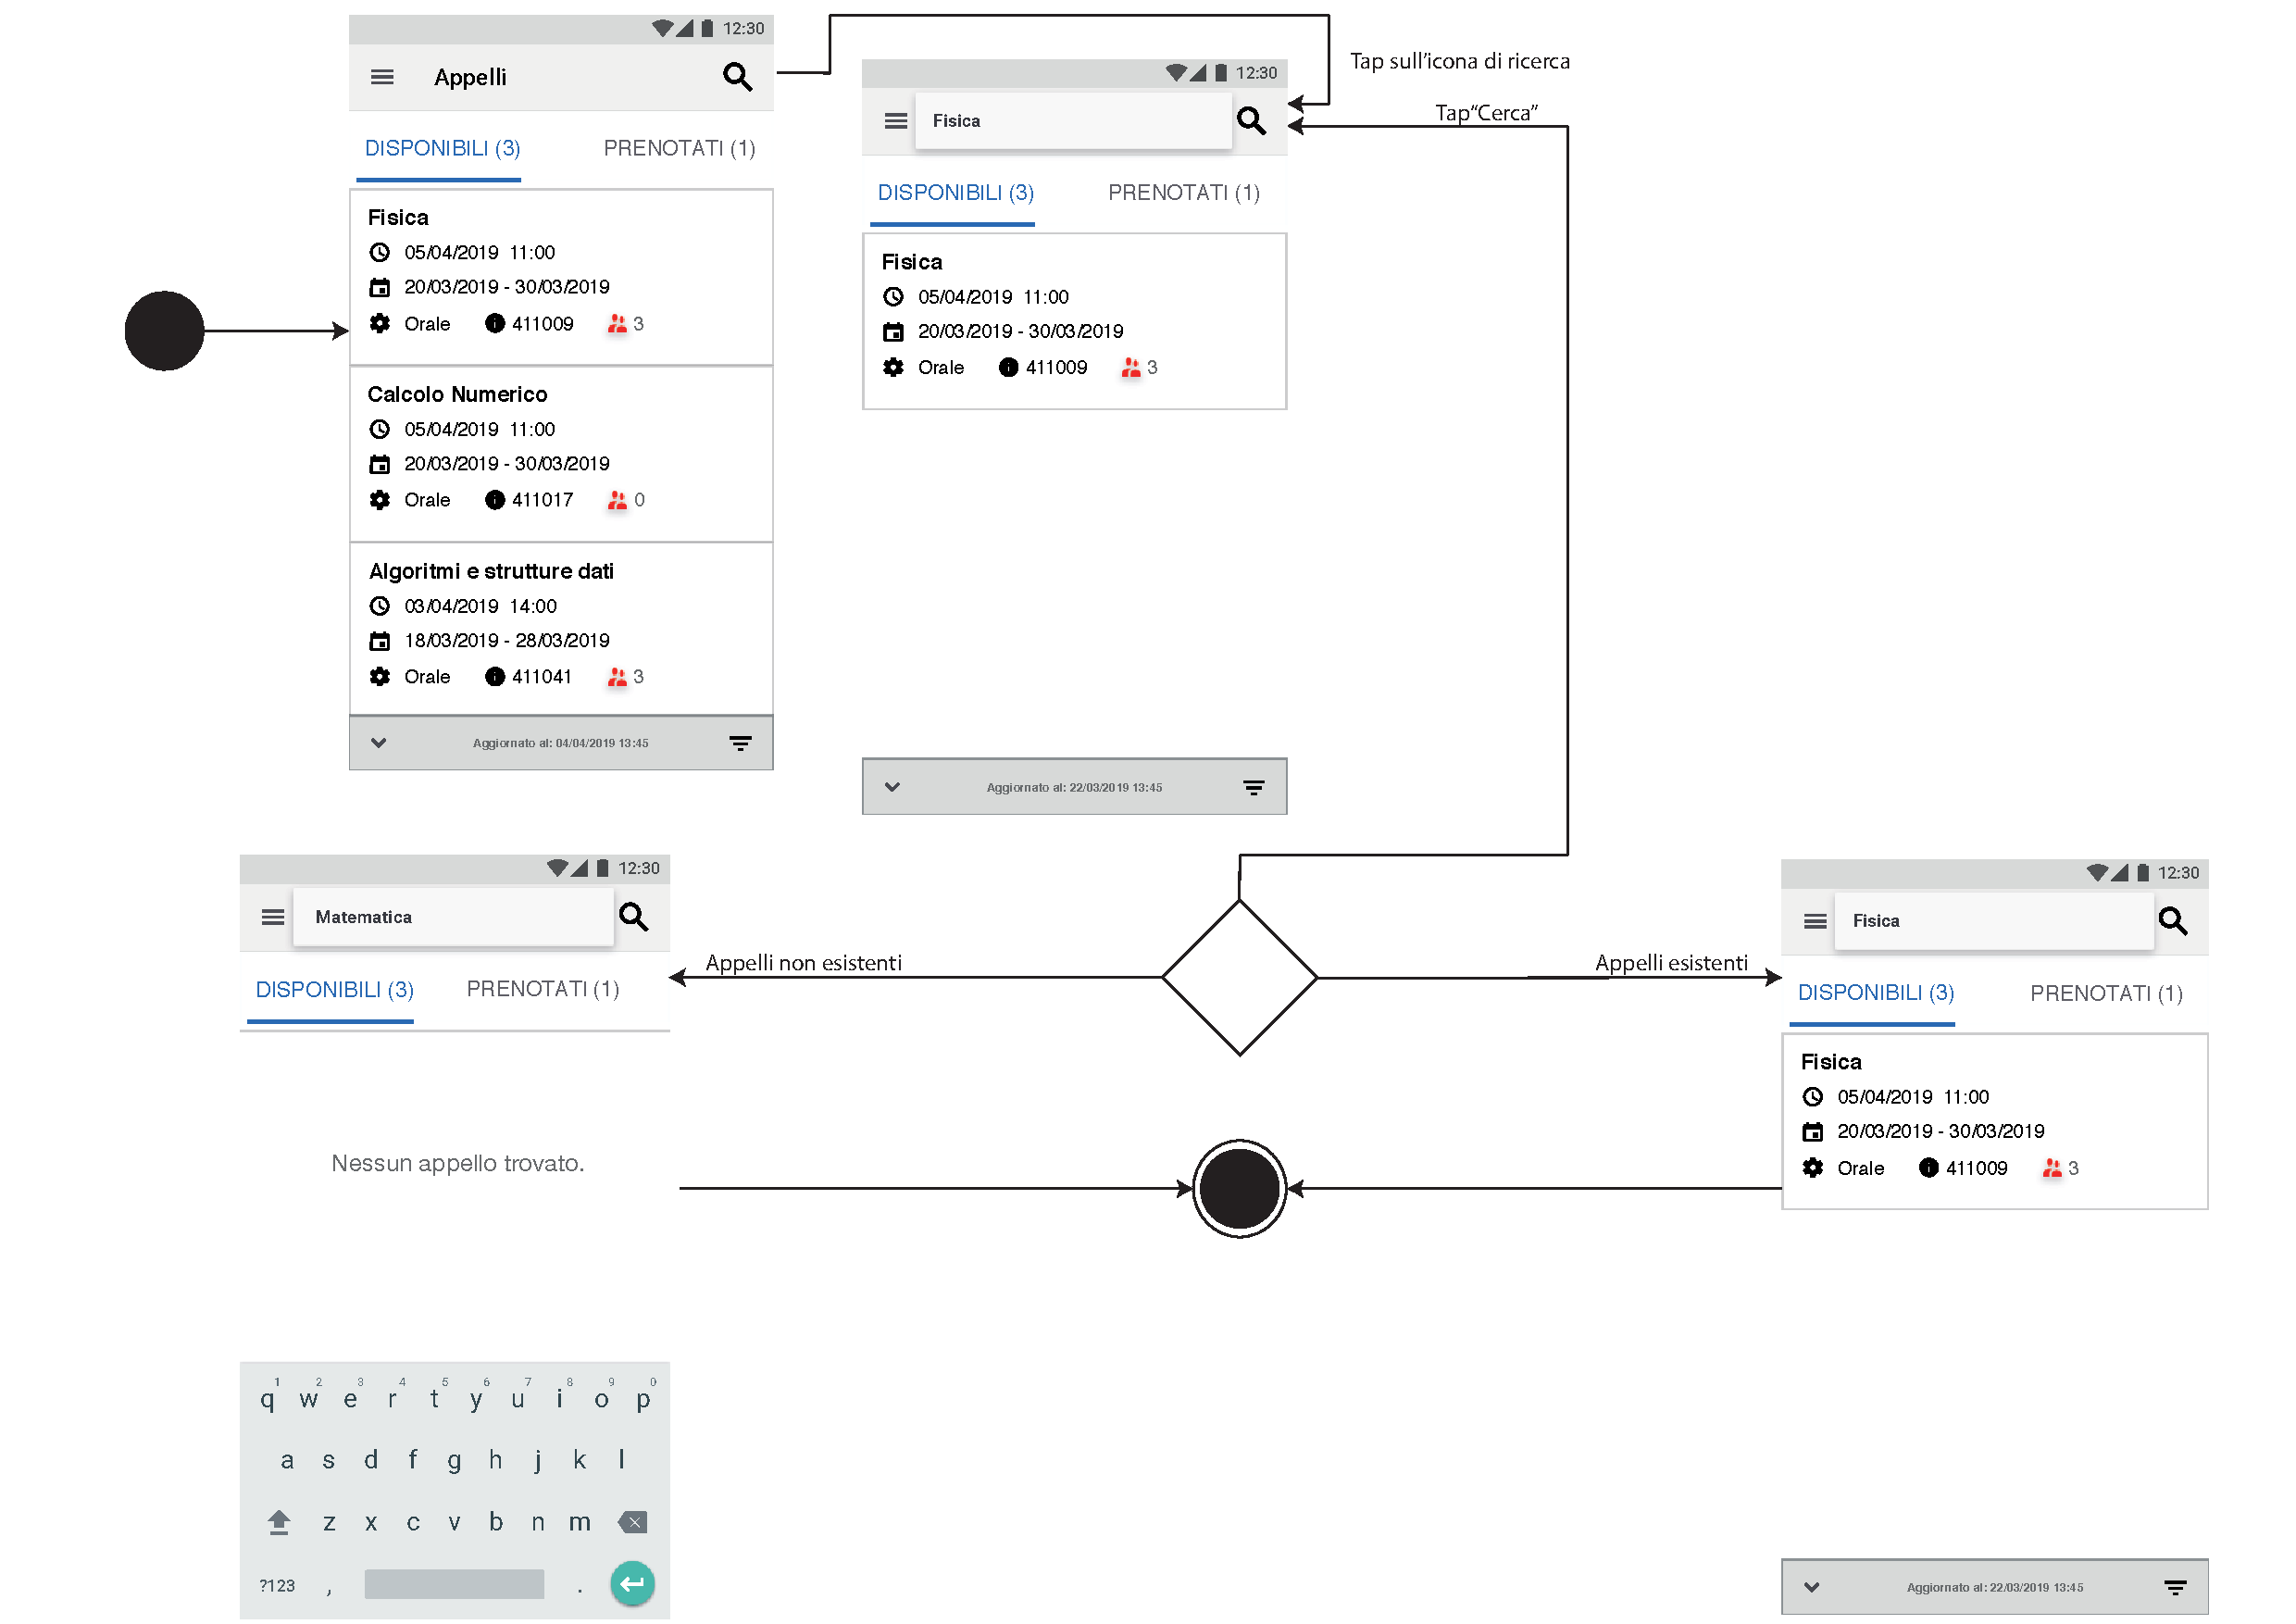
\includegraphics[width=6in]{imgs/gruppo1/activity_diagrams/AD8_Ricerca_appelli.pdf}
\end{center}
\newpage

%%8.6.9 - Filtra appelli disponibili con memorizzazione %%

\subsection{Filtra appelli disponibili con memorizzazione }
\begin{center}
	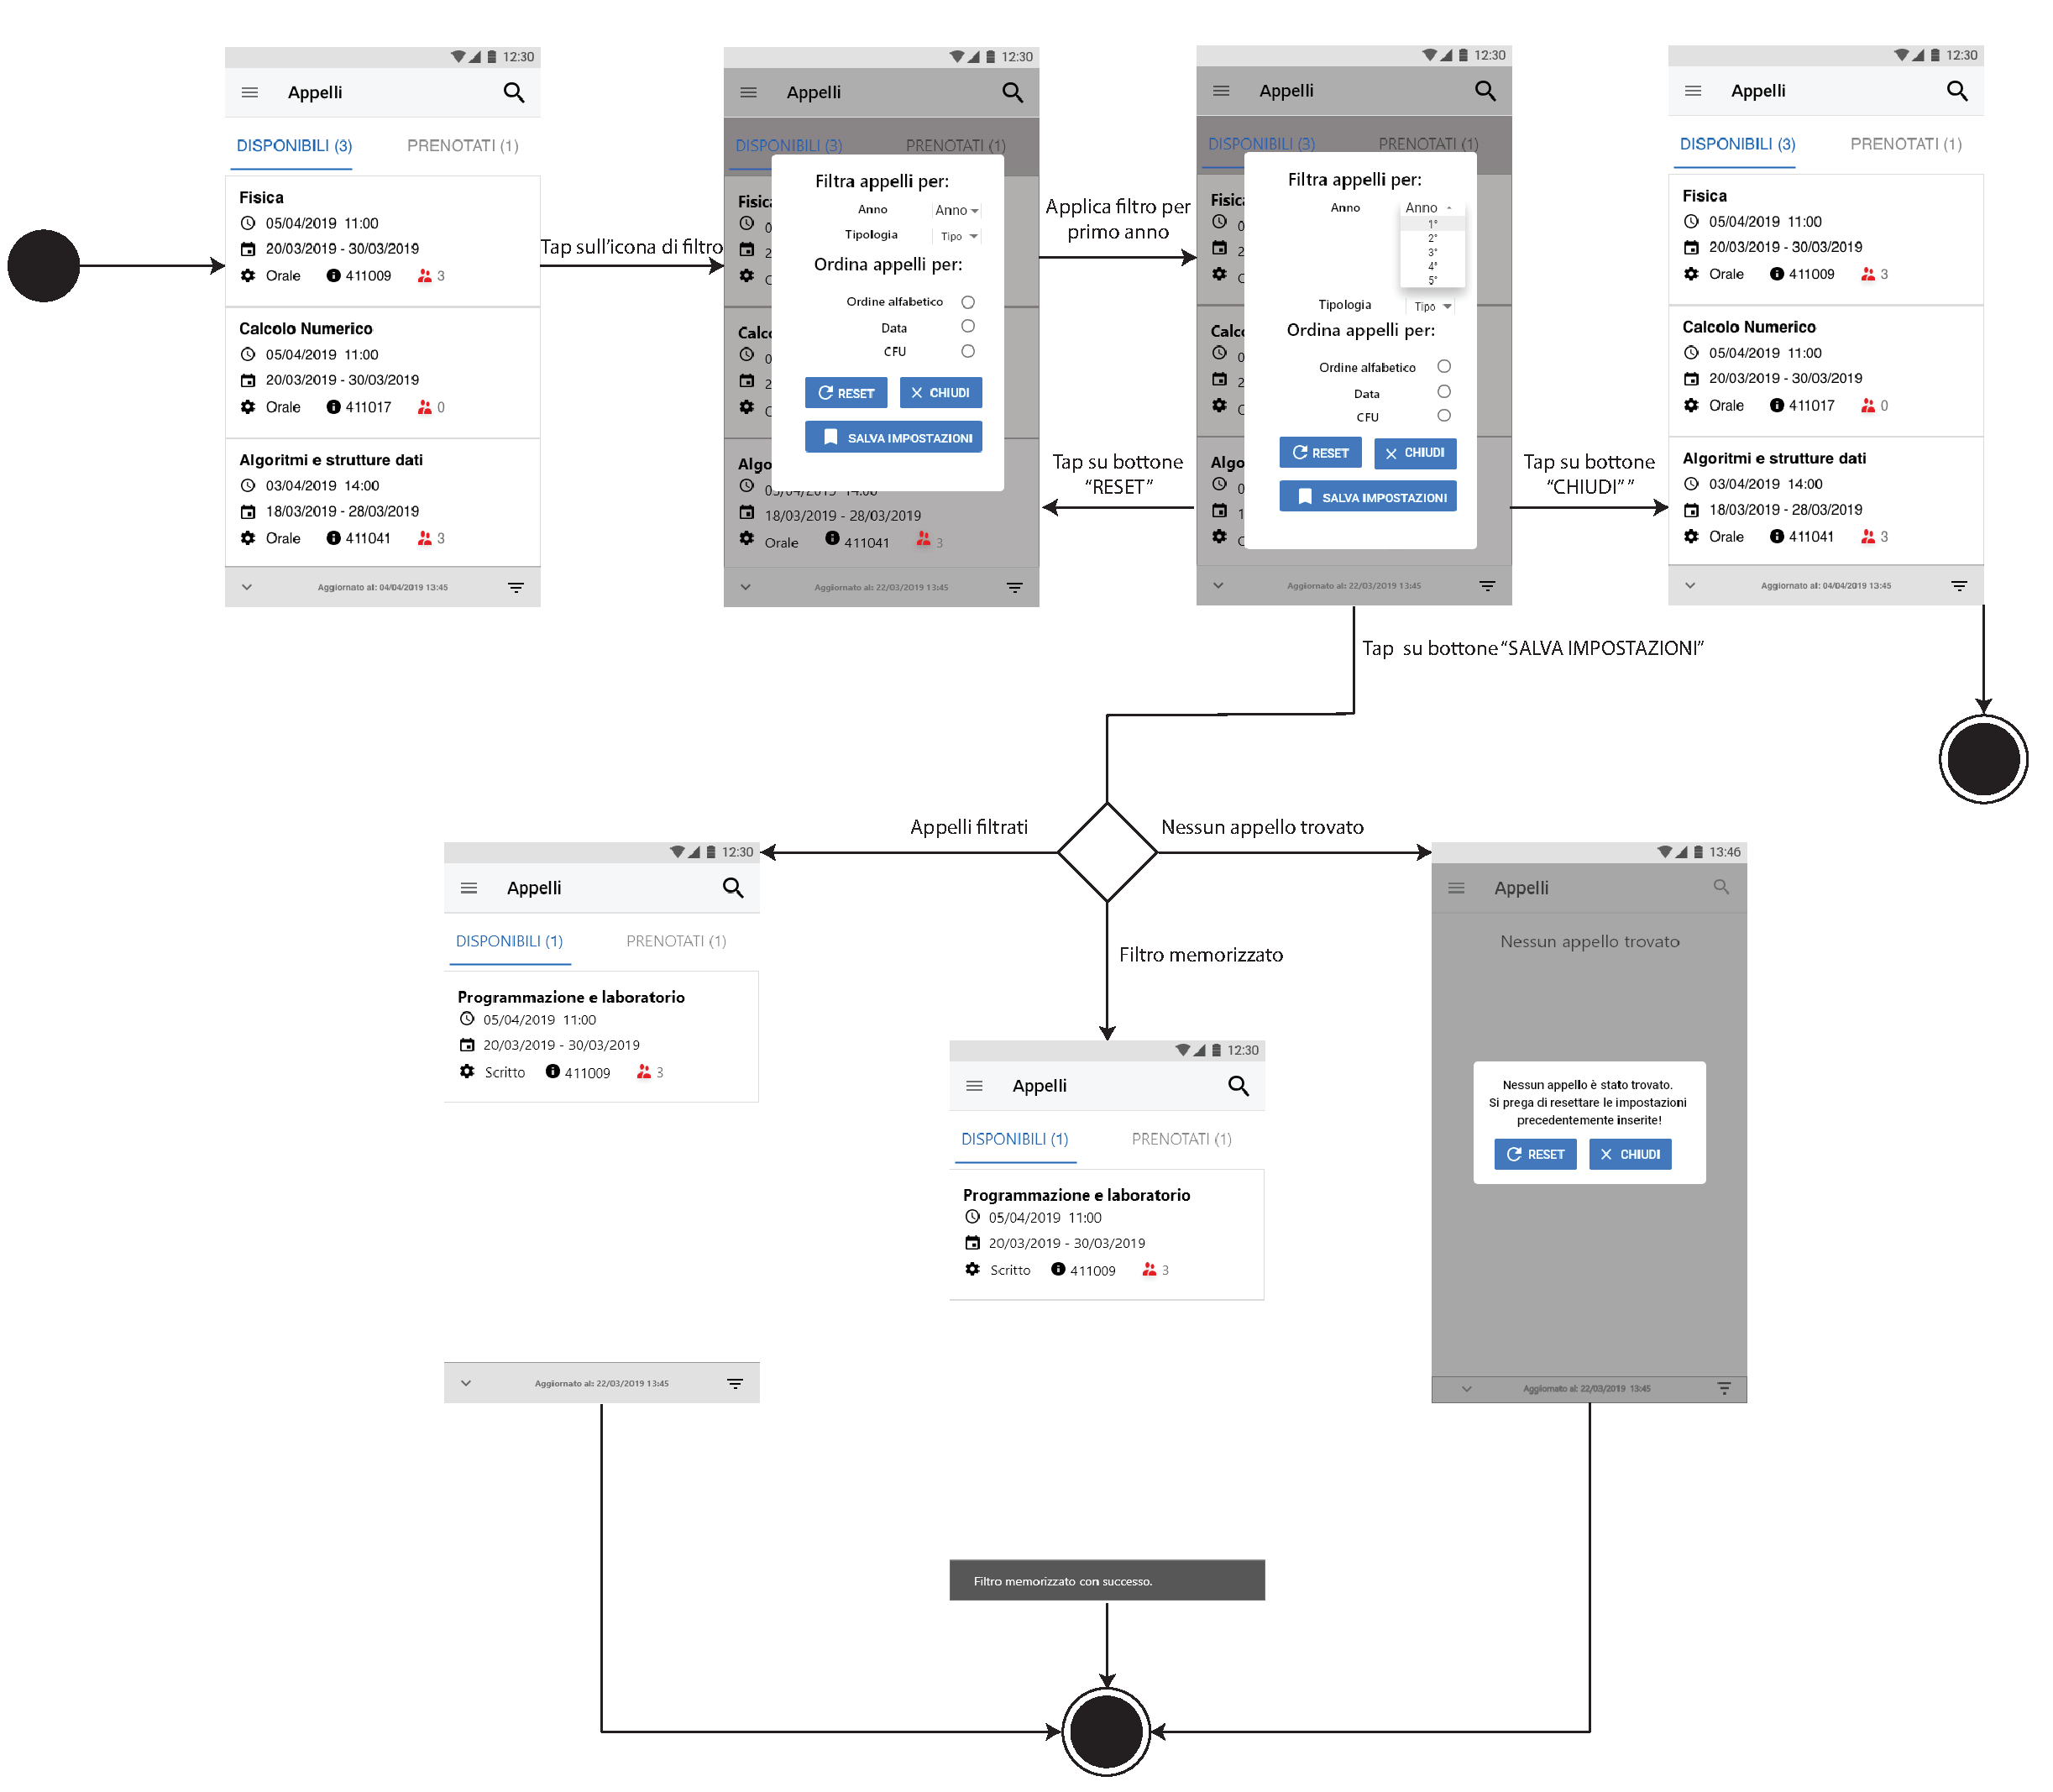
\includegraphics[width=6in]{imgs/gruppo1/activity_diagrams/AD9_filtrati_appelli.pdf}
\end{center}
\newpage

%%8.6.10 - Ordina appelli disponibili con memorizzazione%%

\subsection{Ordina appelli disponibili con memorizzazione }
\begin{center}
	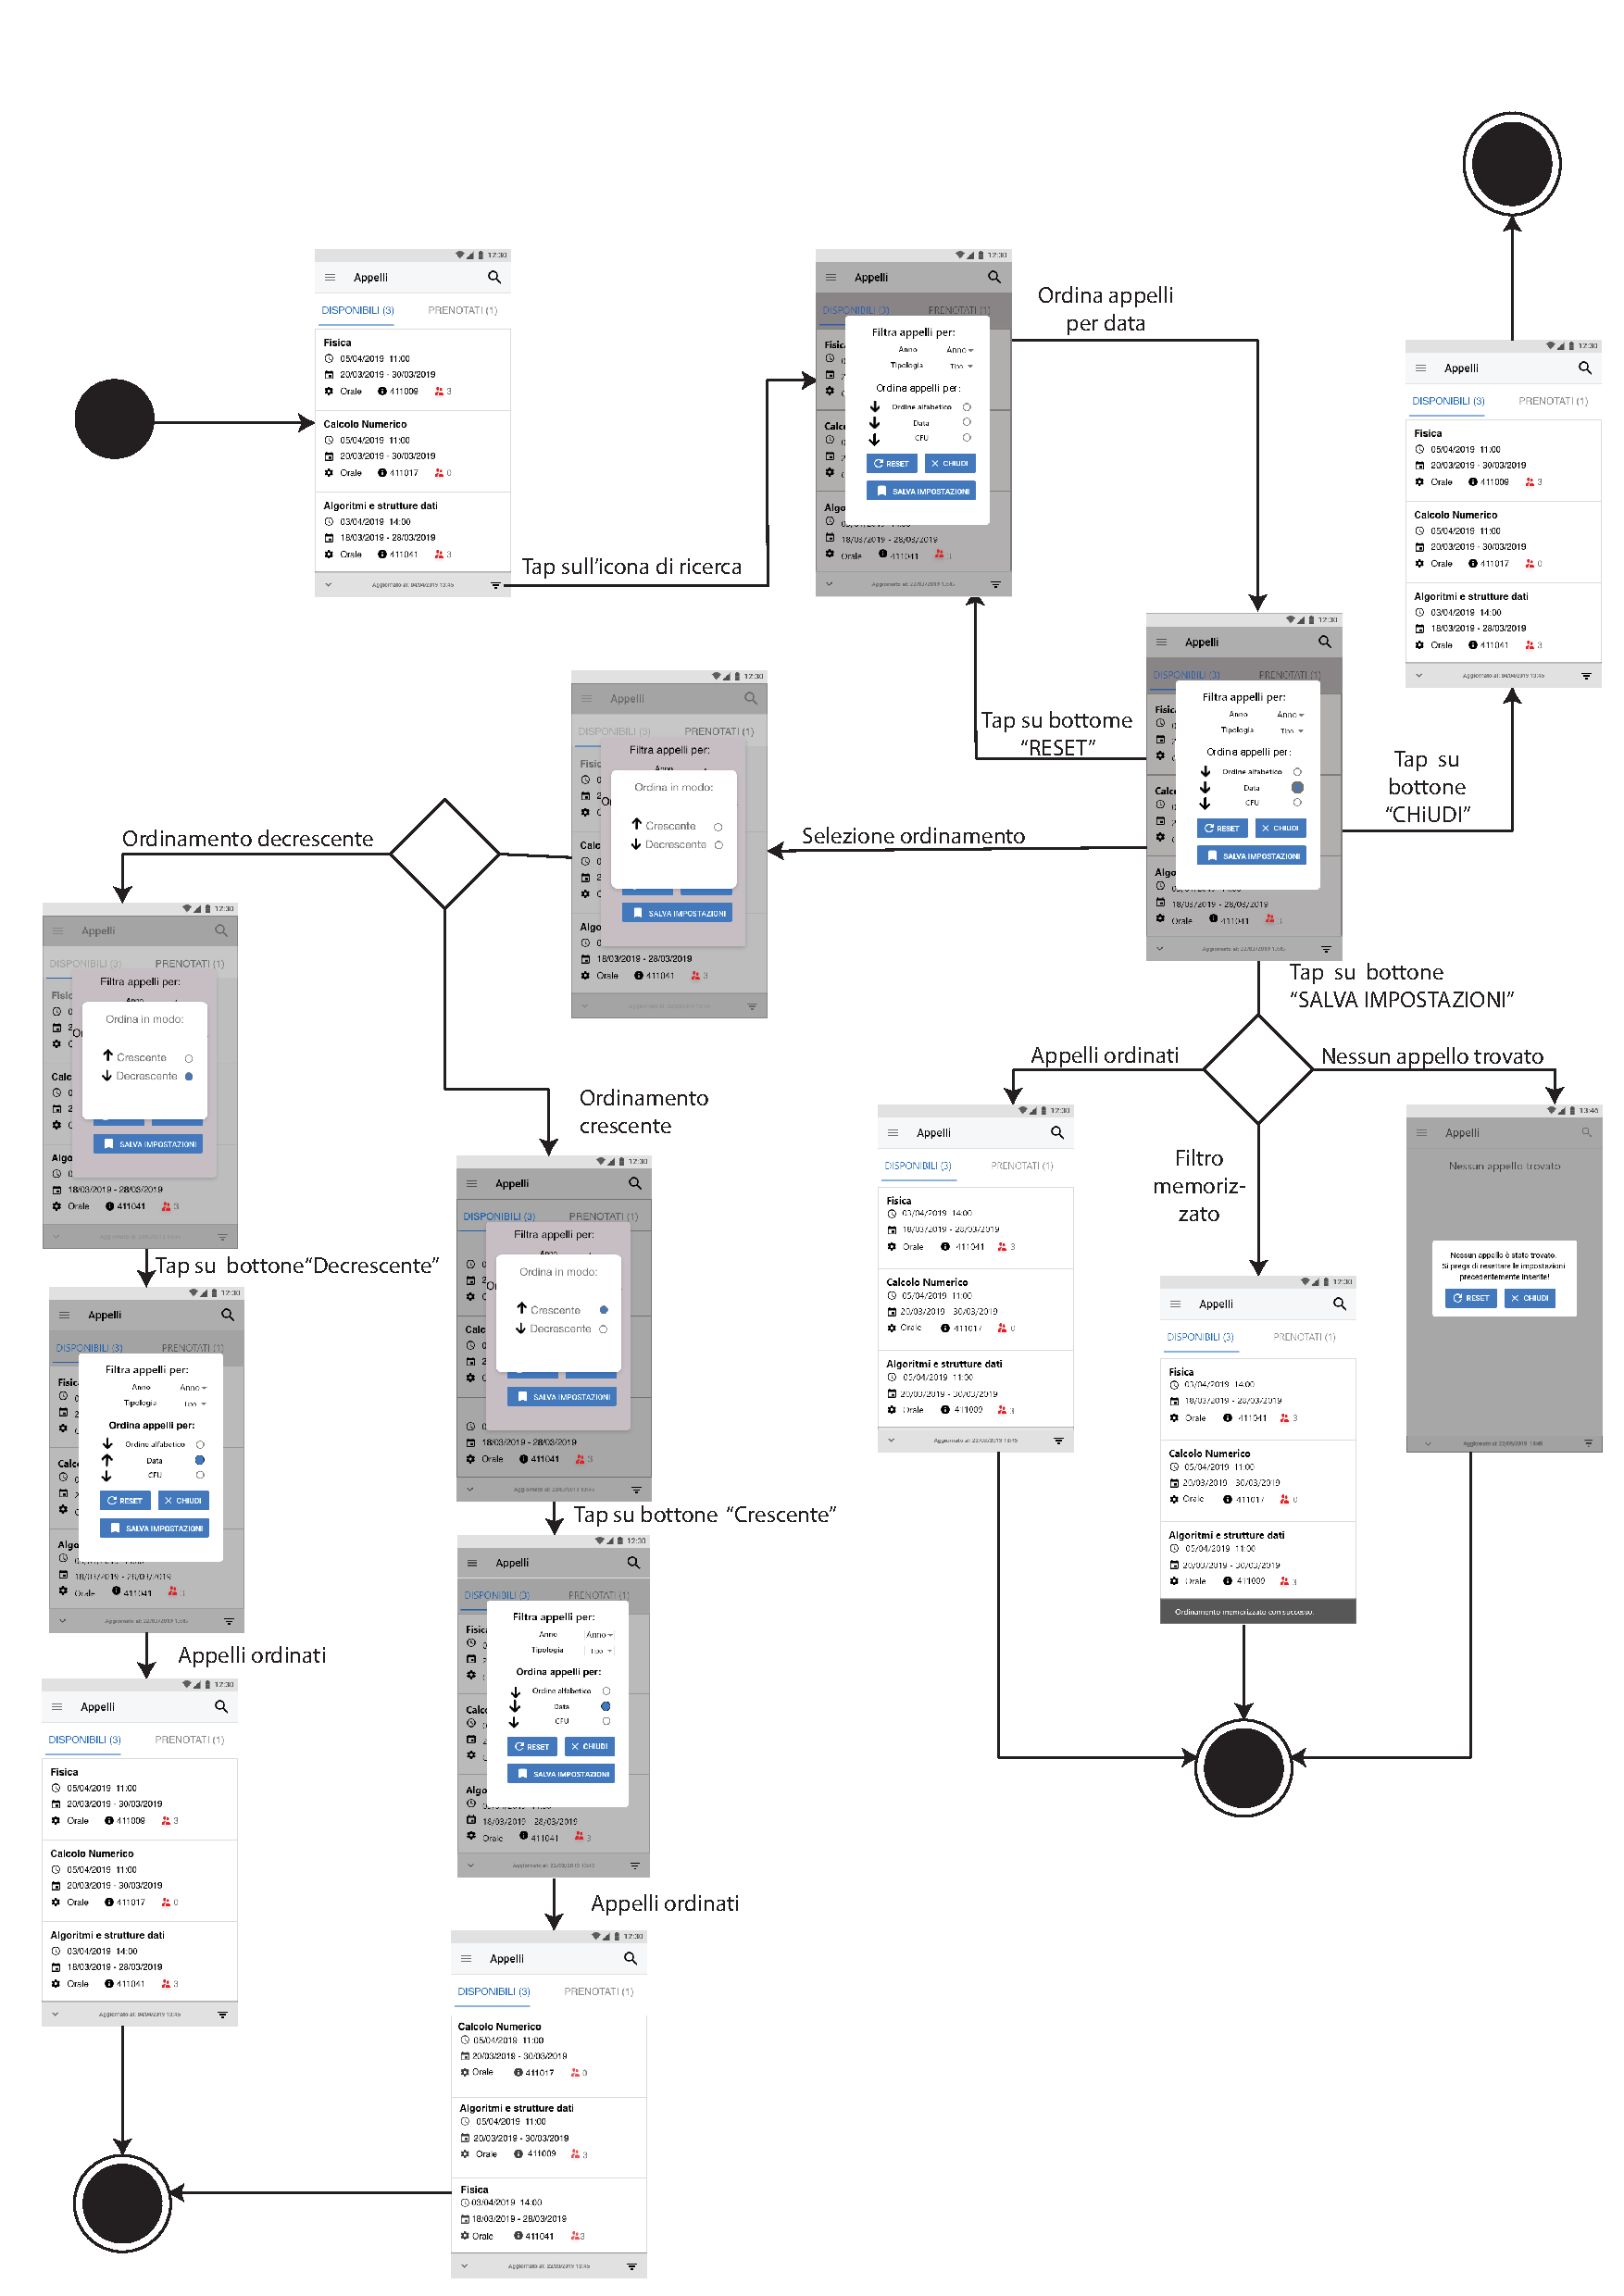
\includegraphics[width=6in]{imgs/gruppo1/activity_diagrams/AD10_ordina_appelli.pdf}
\end{center}
\newpage

%%8.6.11 - Prenota appello%%

\subsection{Prenota appello }
\begin{center}
	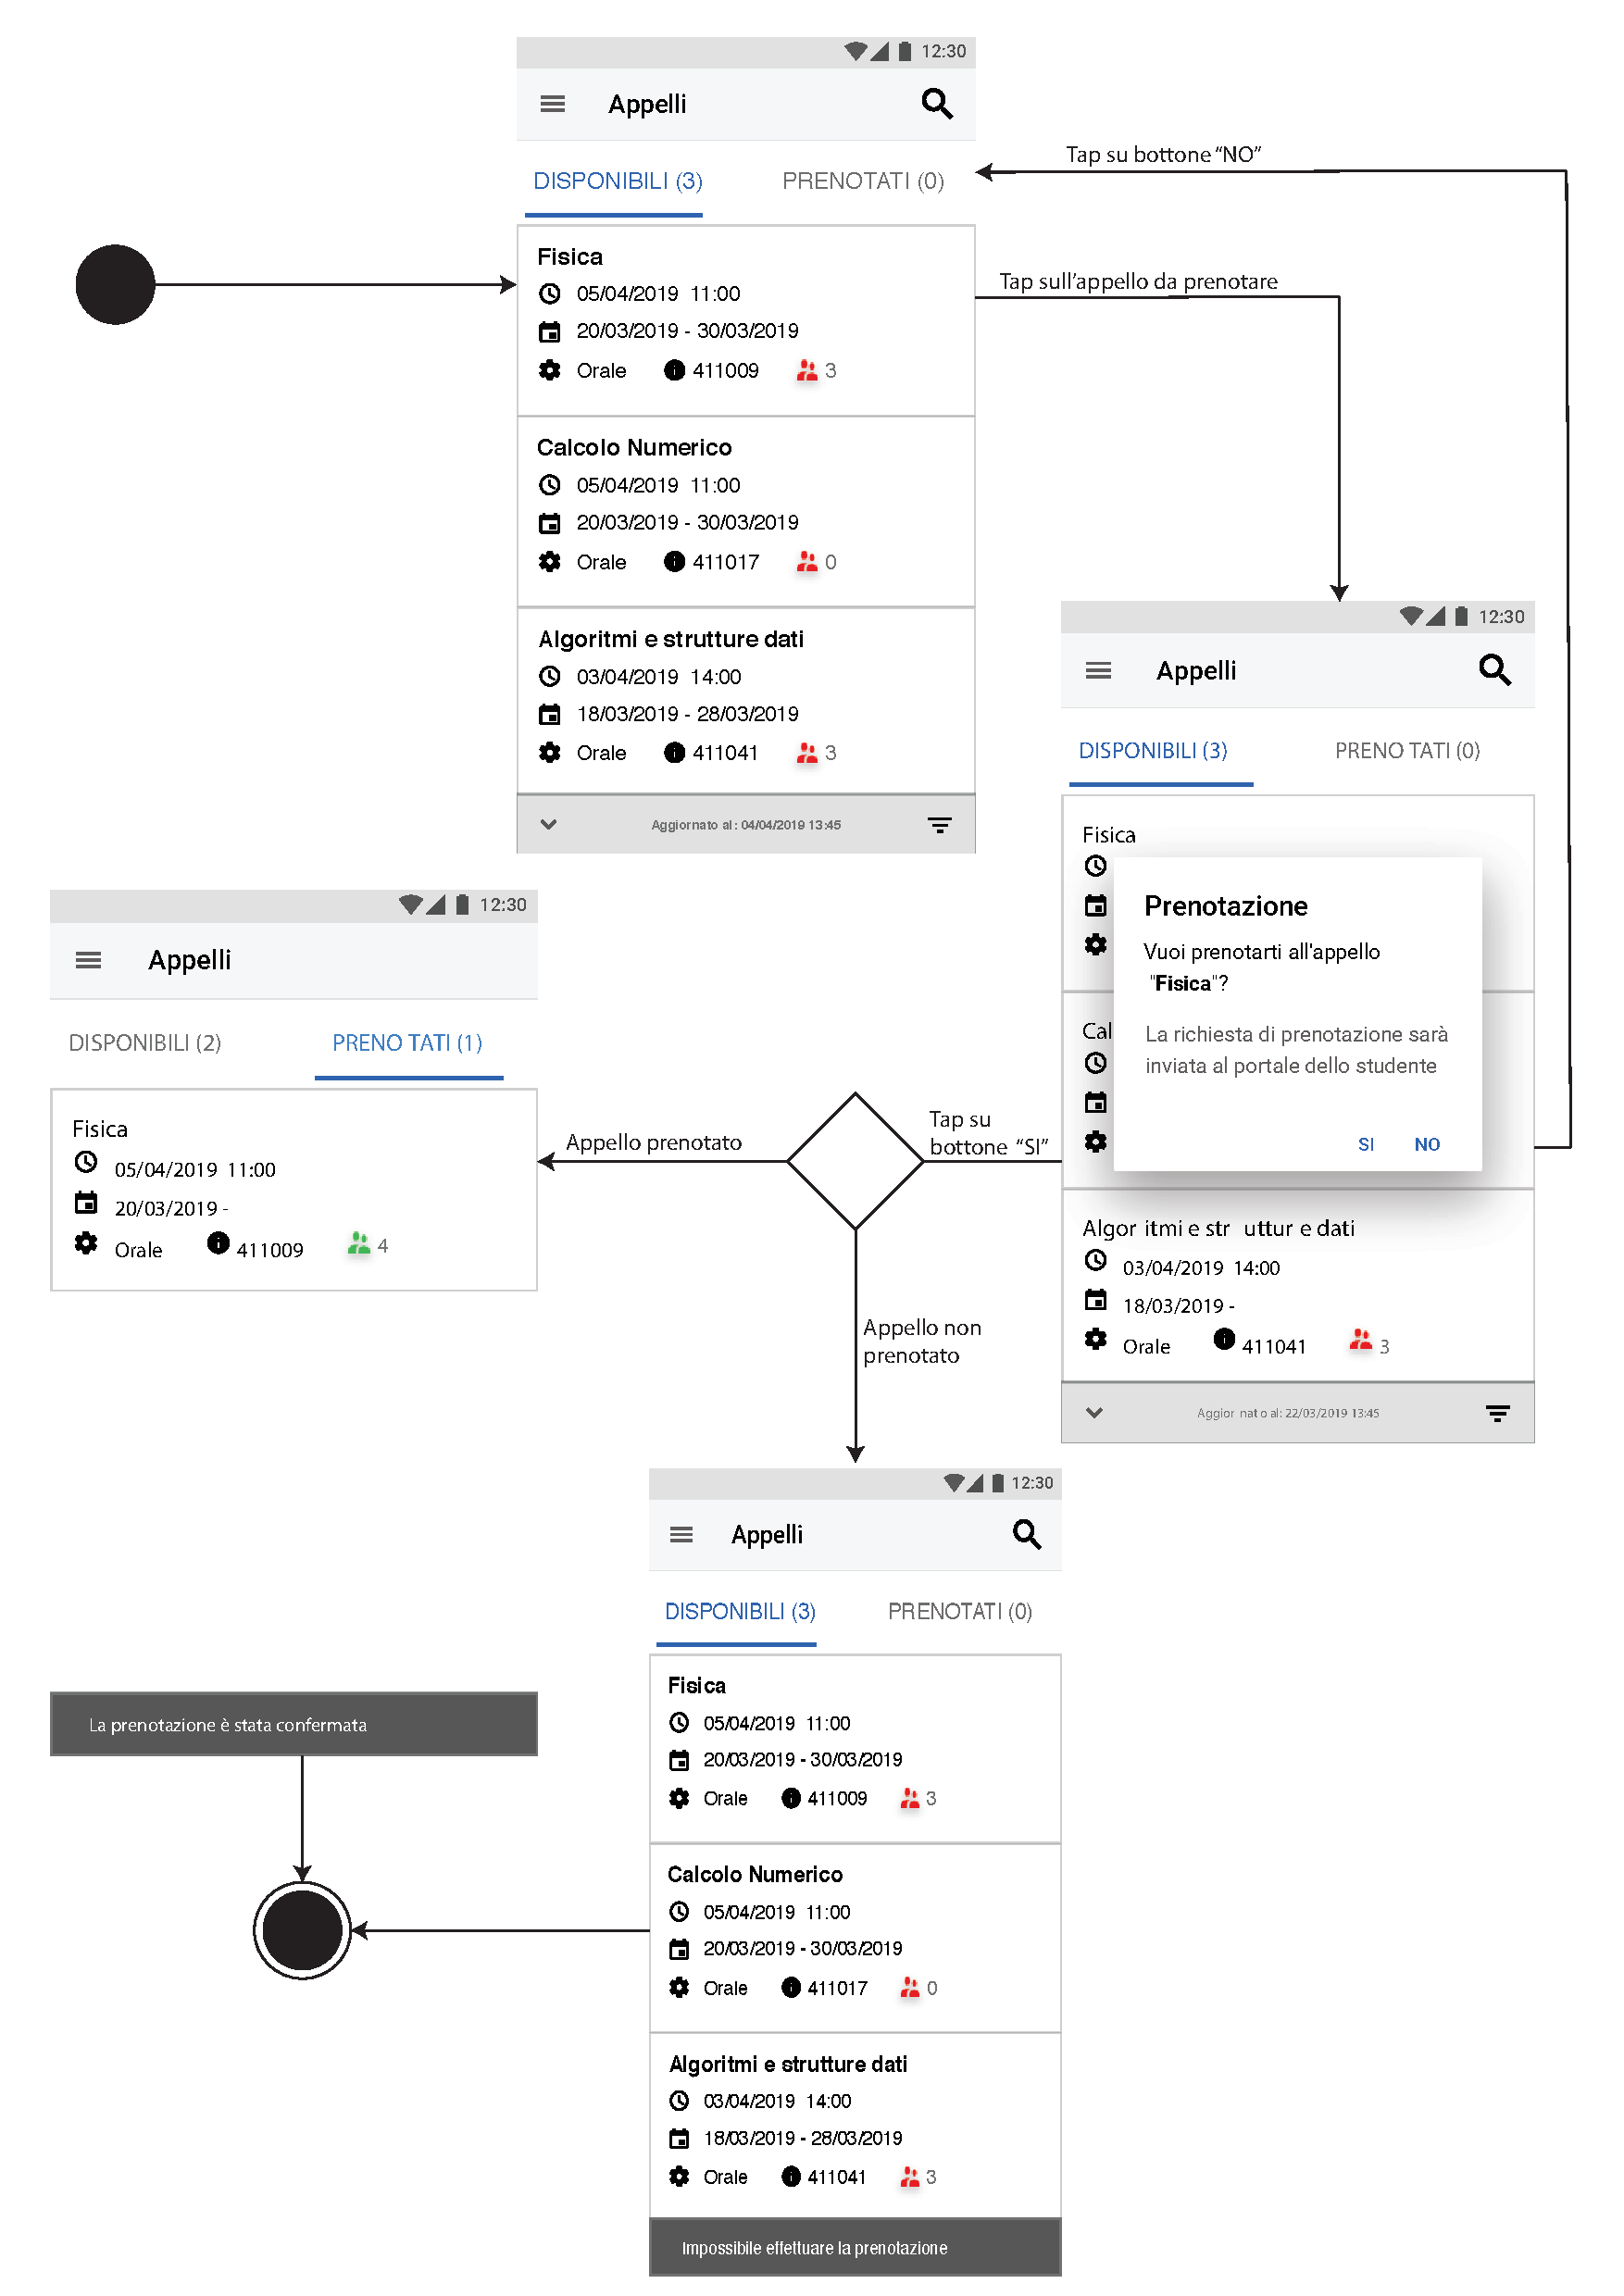
\includegraphics[width=6in]{imgs/gruppo1/activity_diagrams/AD11_prenota_apppello.pdf}
\end{center}
\newpage

%%8.6.12 - Cancella prenotazione%%

\subsection{Cancella prenotazione}
\begin{center}
	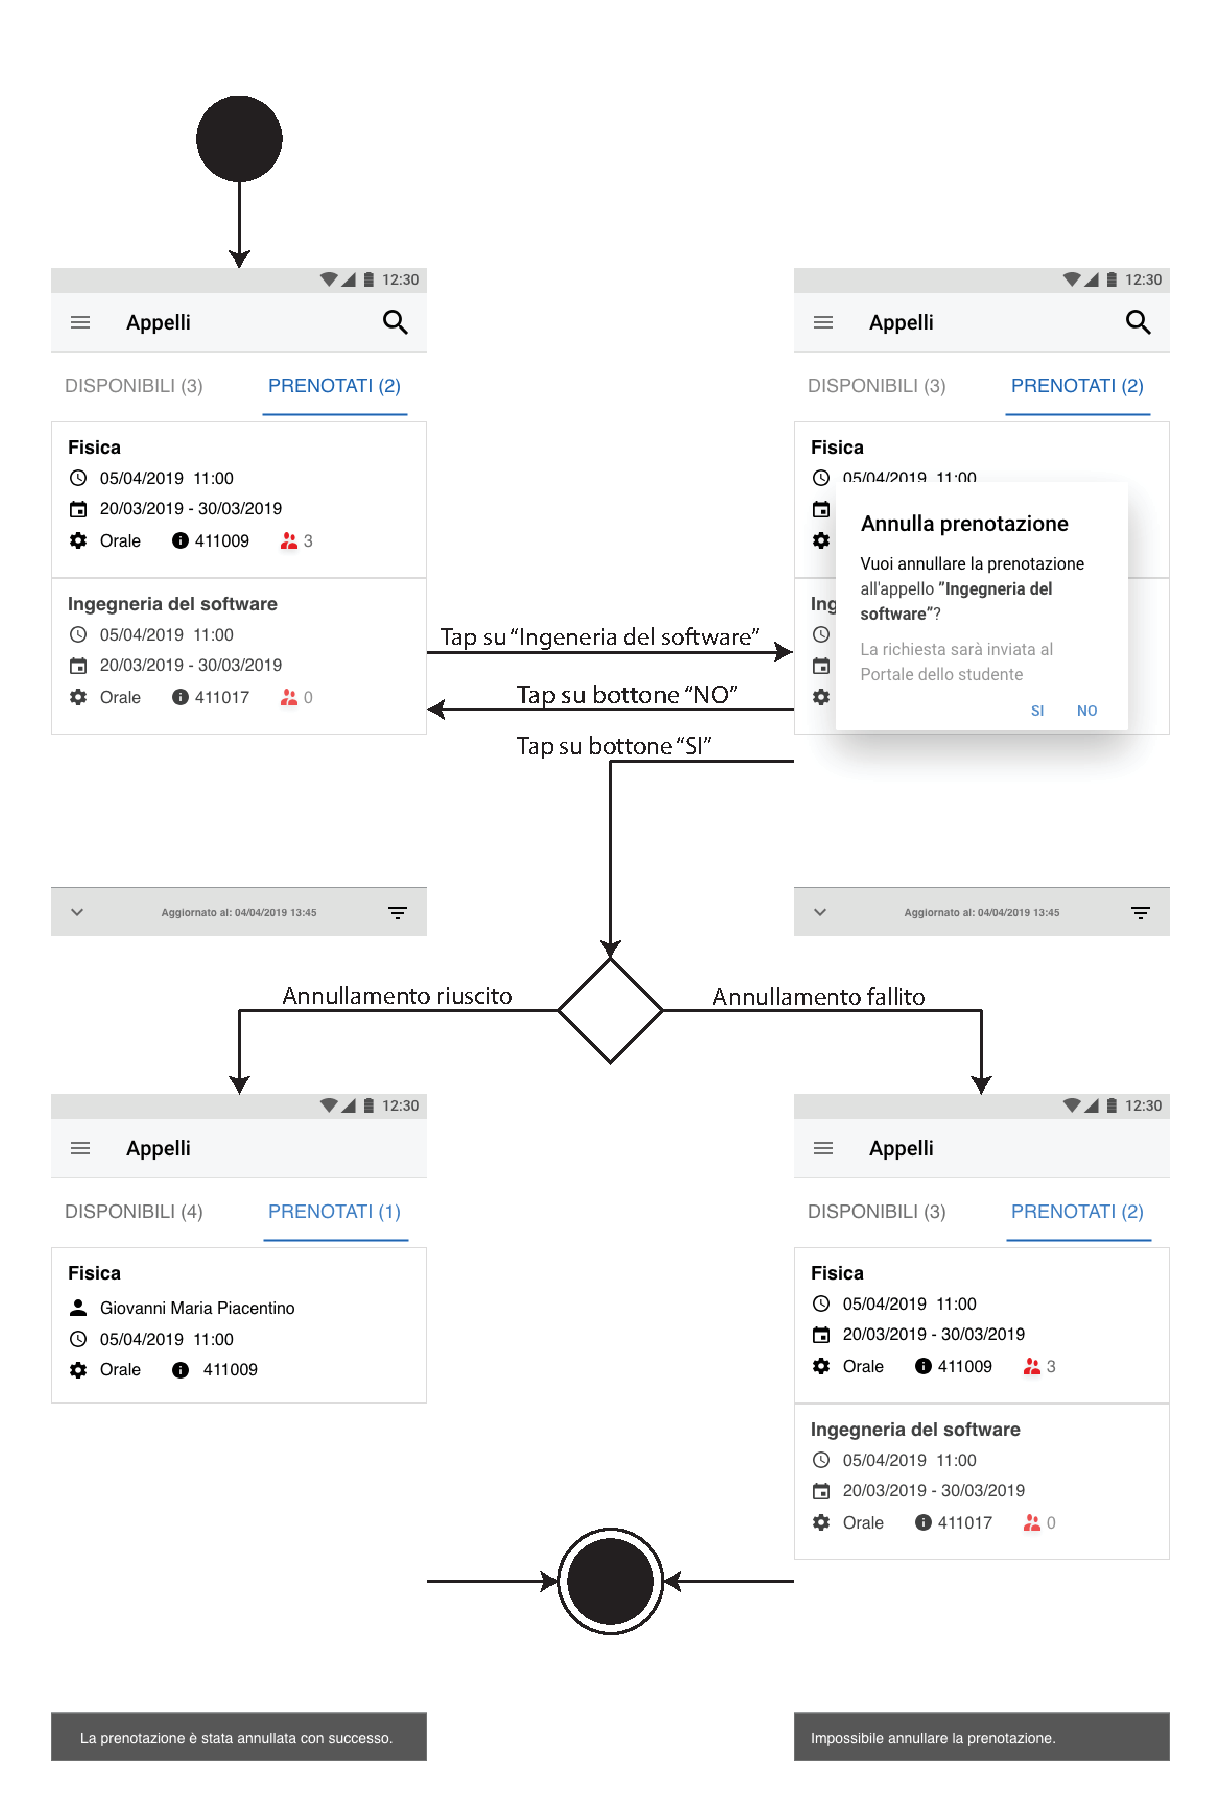
\includegraphics[width=6in]{imgs/gruppo1/activity_diagrams/AD12_cancella_prenotazione.pdf}
\end{center}
\newpage

%%8.6.13 - Visualizza elenco file%%

\subsection{Visualizza elenco file}
\begin{center}
	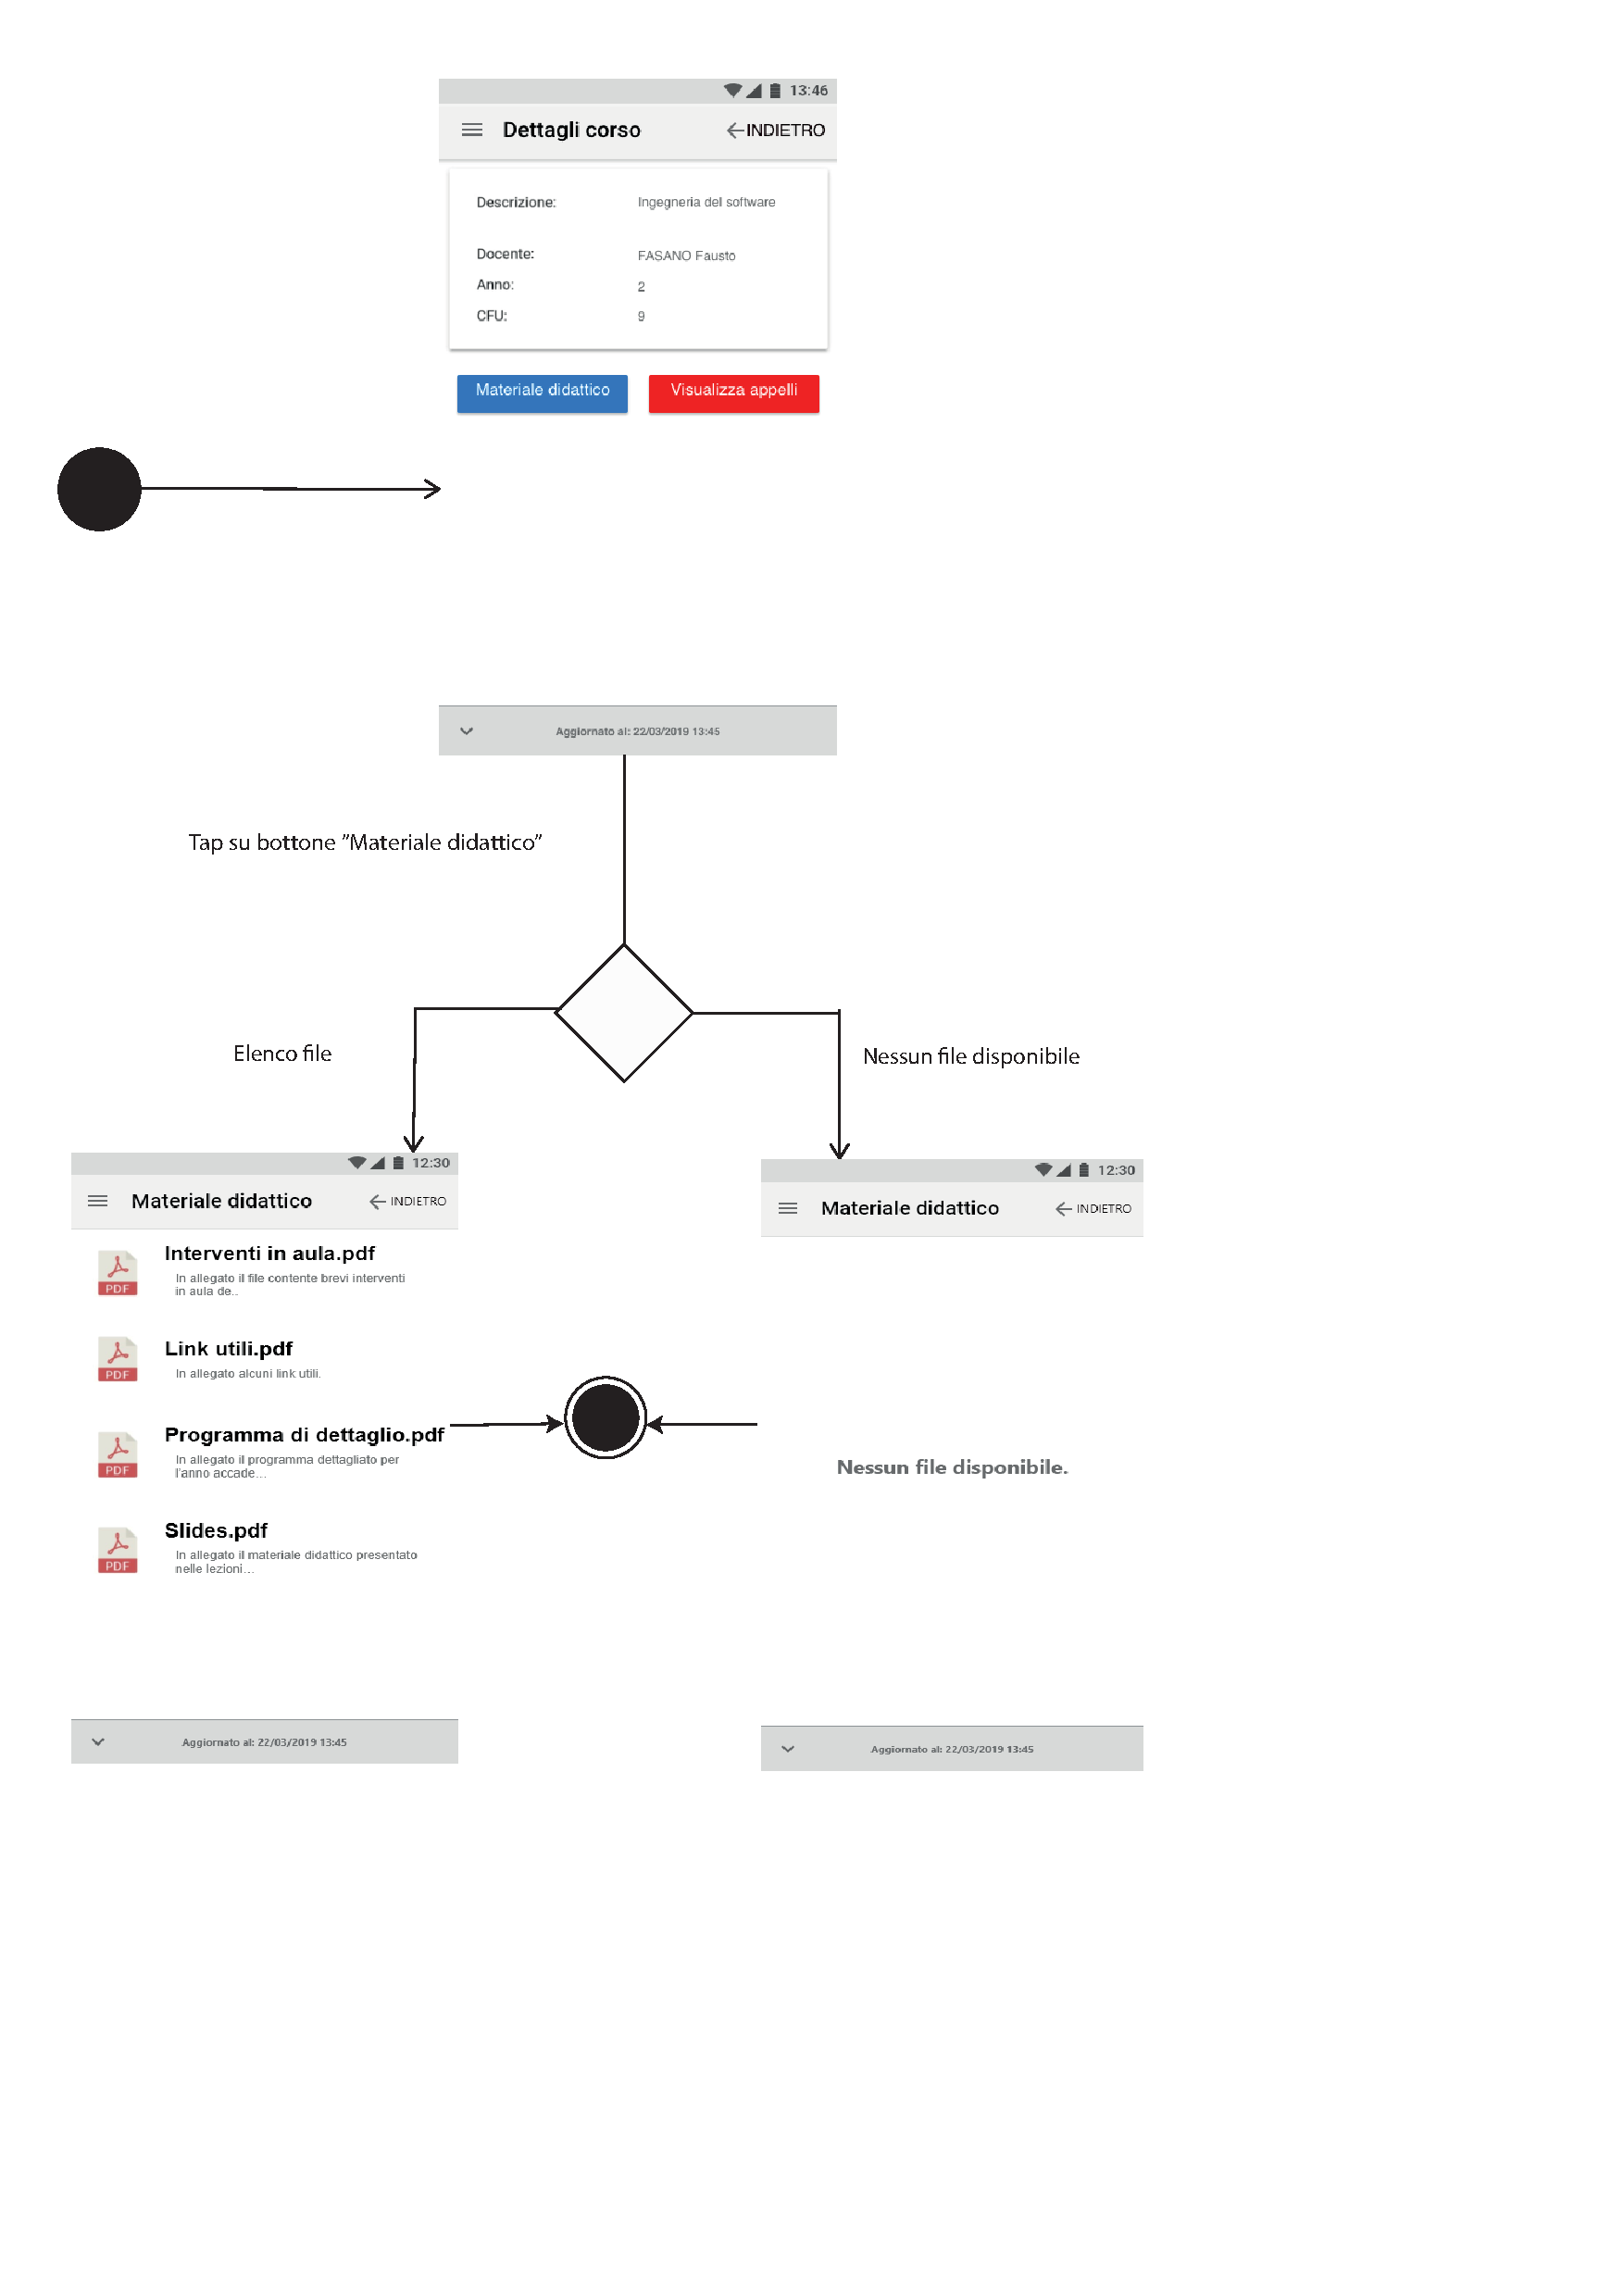
\includegraphics[width=6in]{imgs/gruppo1/activity_diagrams/AD13_viasualizza_elenco_file.pdf}
\end{center}
\newpage

%%8.6.14 - Ricerca files%%

\subsection{Ricerca files}
\begin{center}
	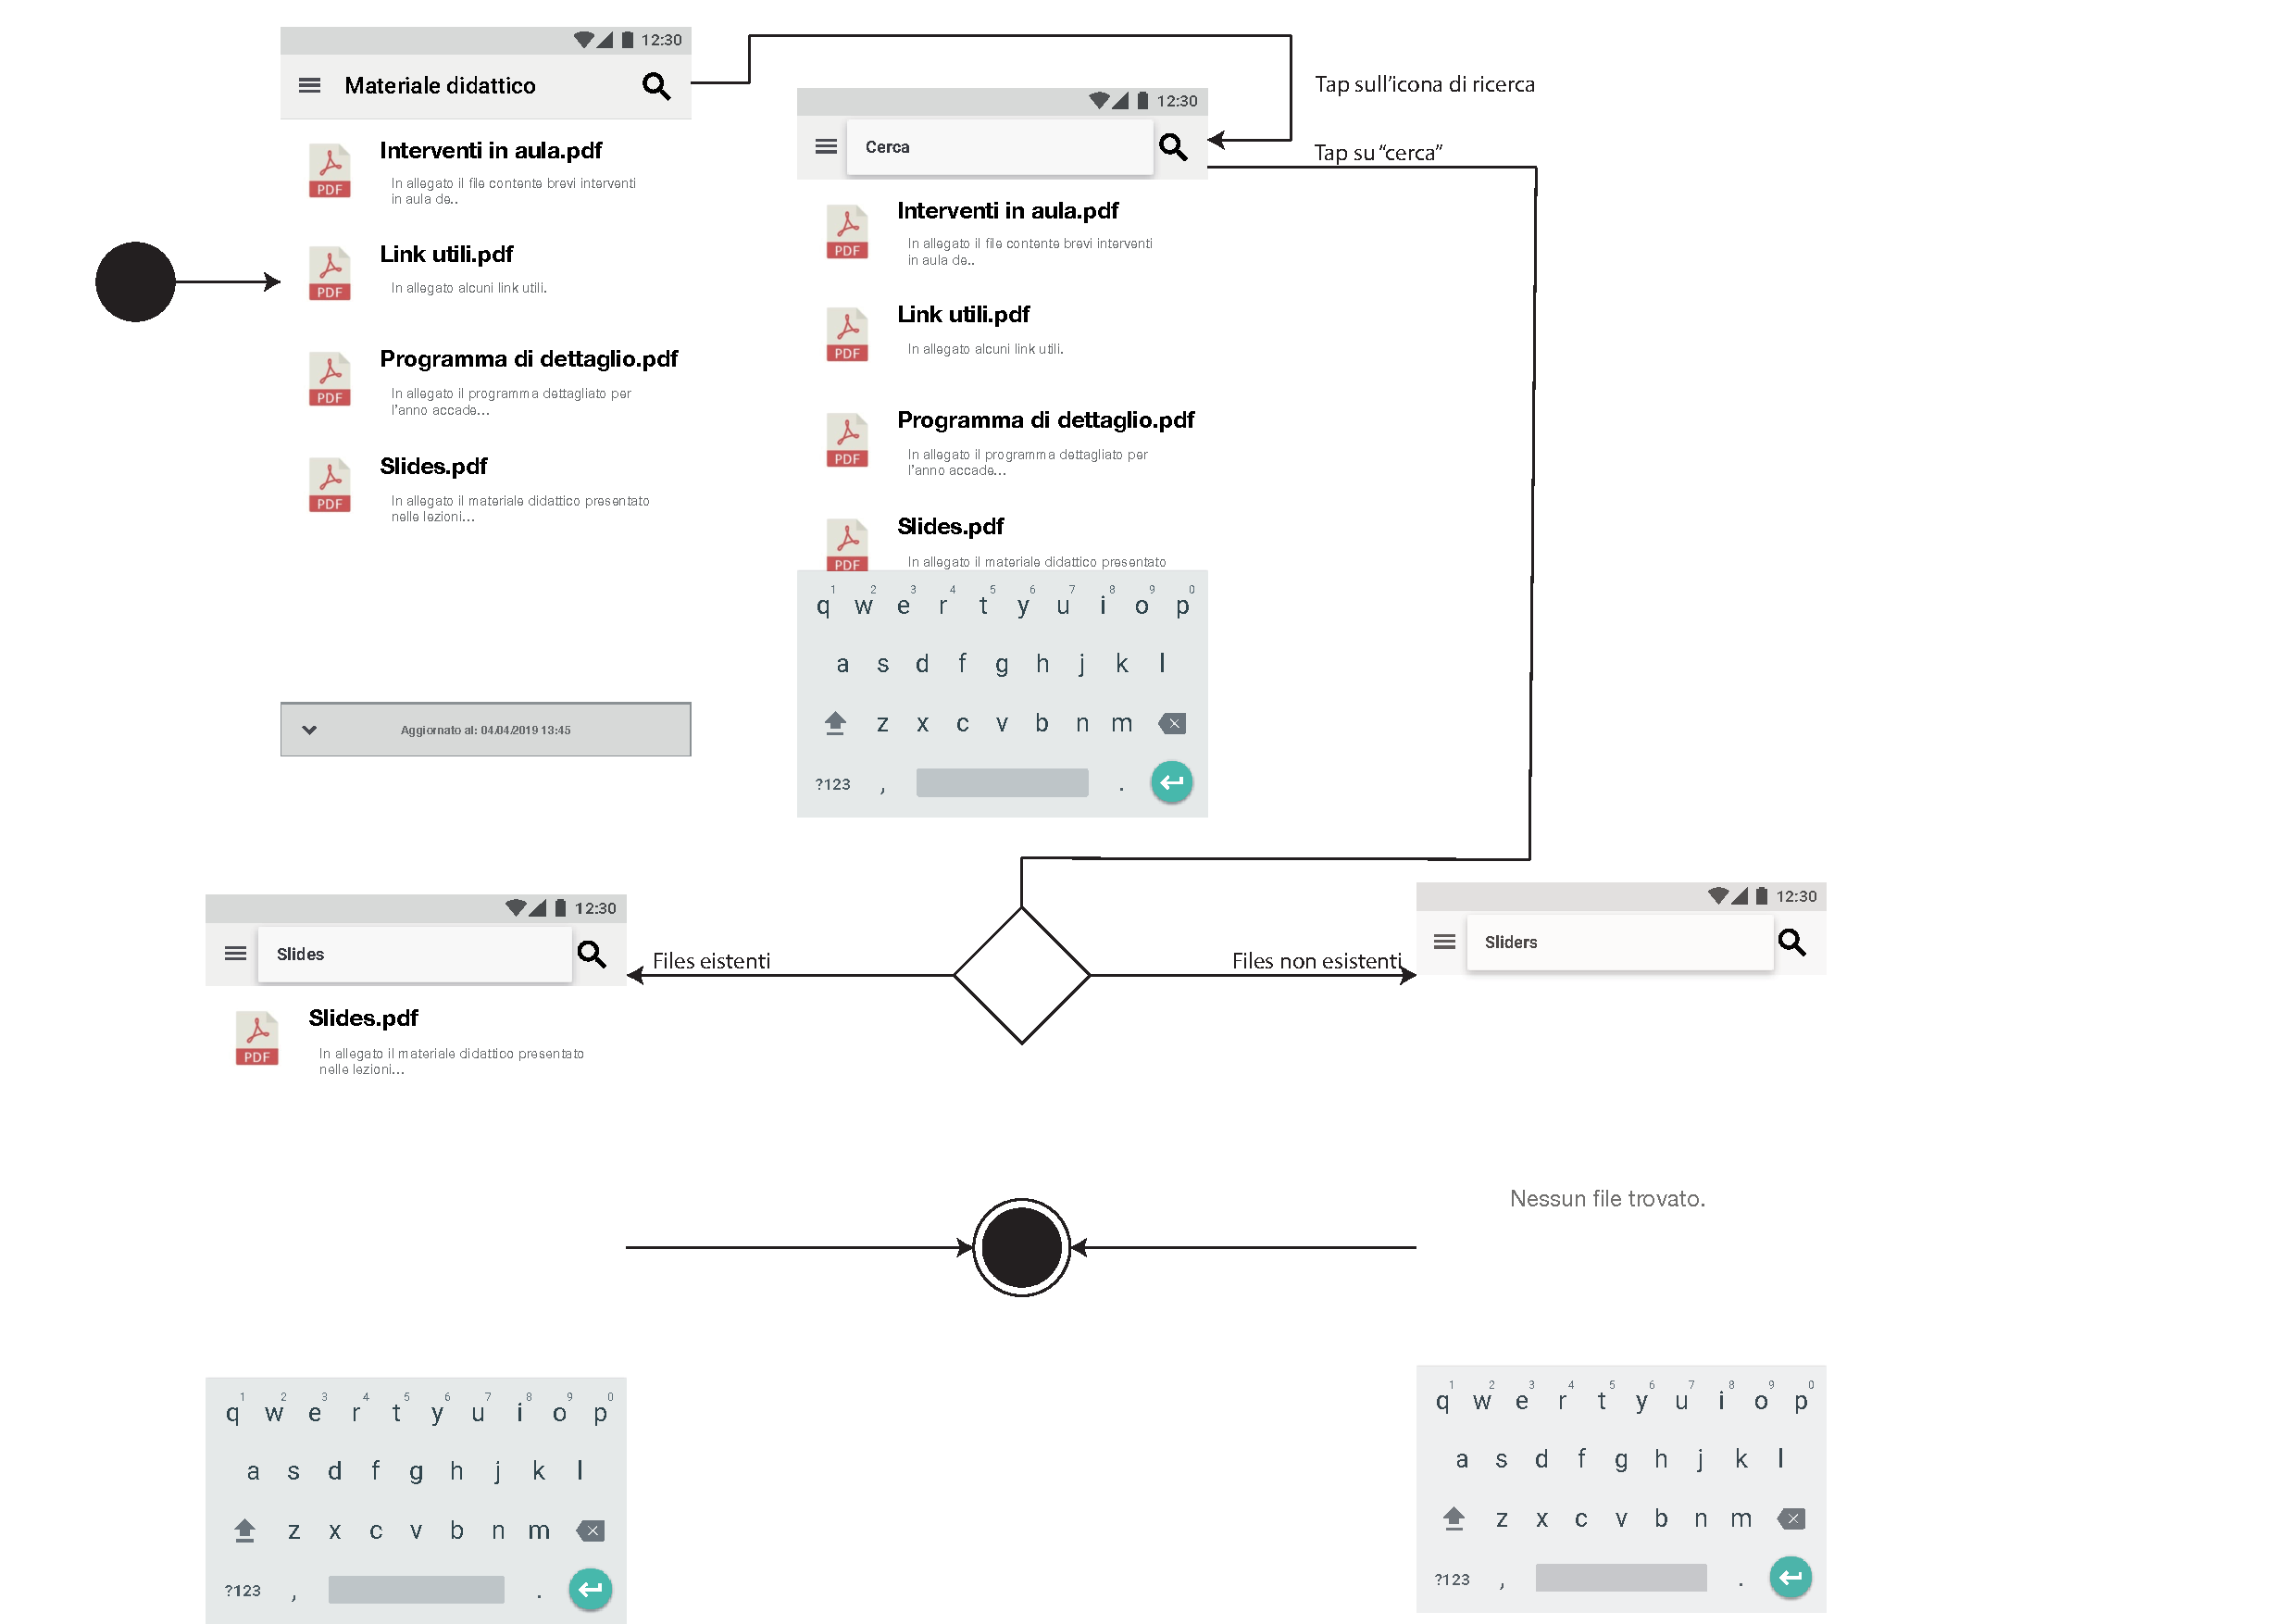
\includegraphics[width=6in]{imgs/gruppo1/activity_diagrams/AD14_ricerca_file.pdf}
\end{center}
\newpage

%%8.6.15 - Visualizza dettagli file%%

\subsection{Visualizza dettagli file}
\begin{center}
	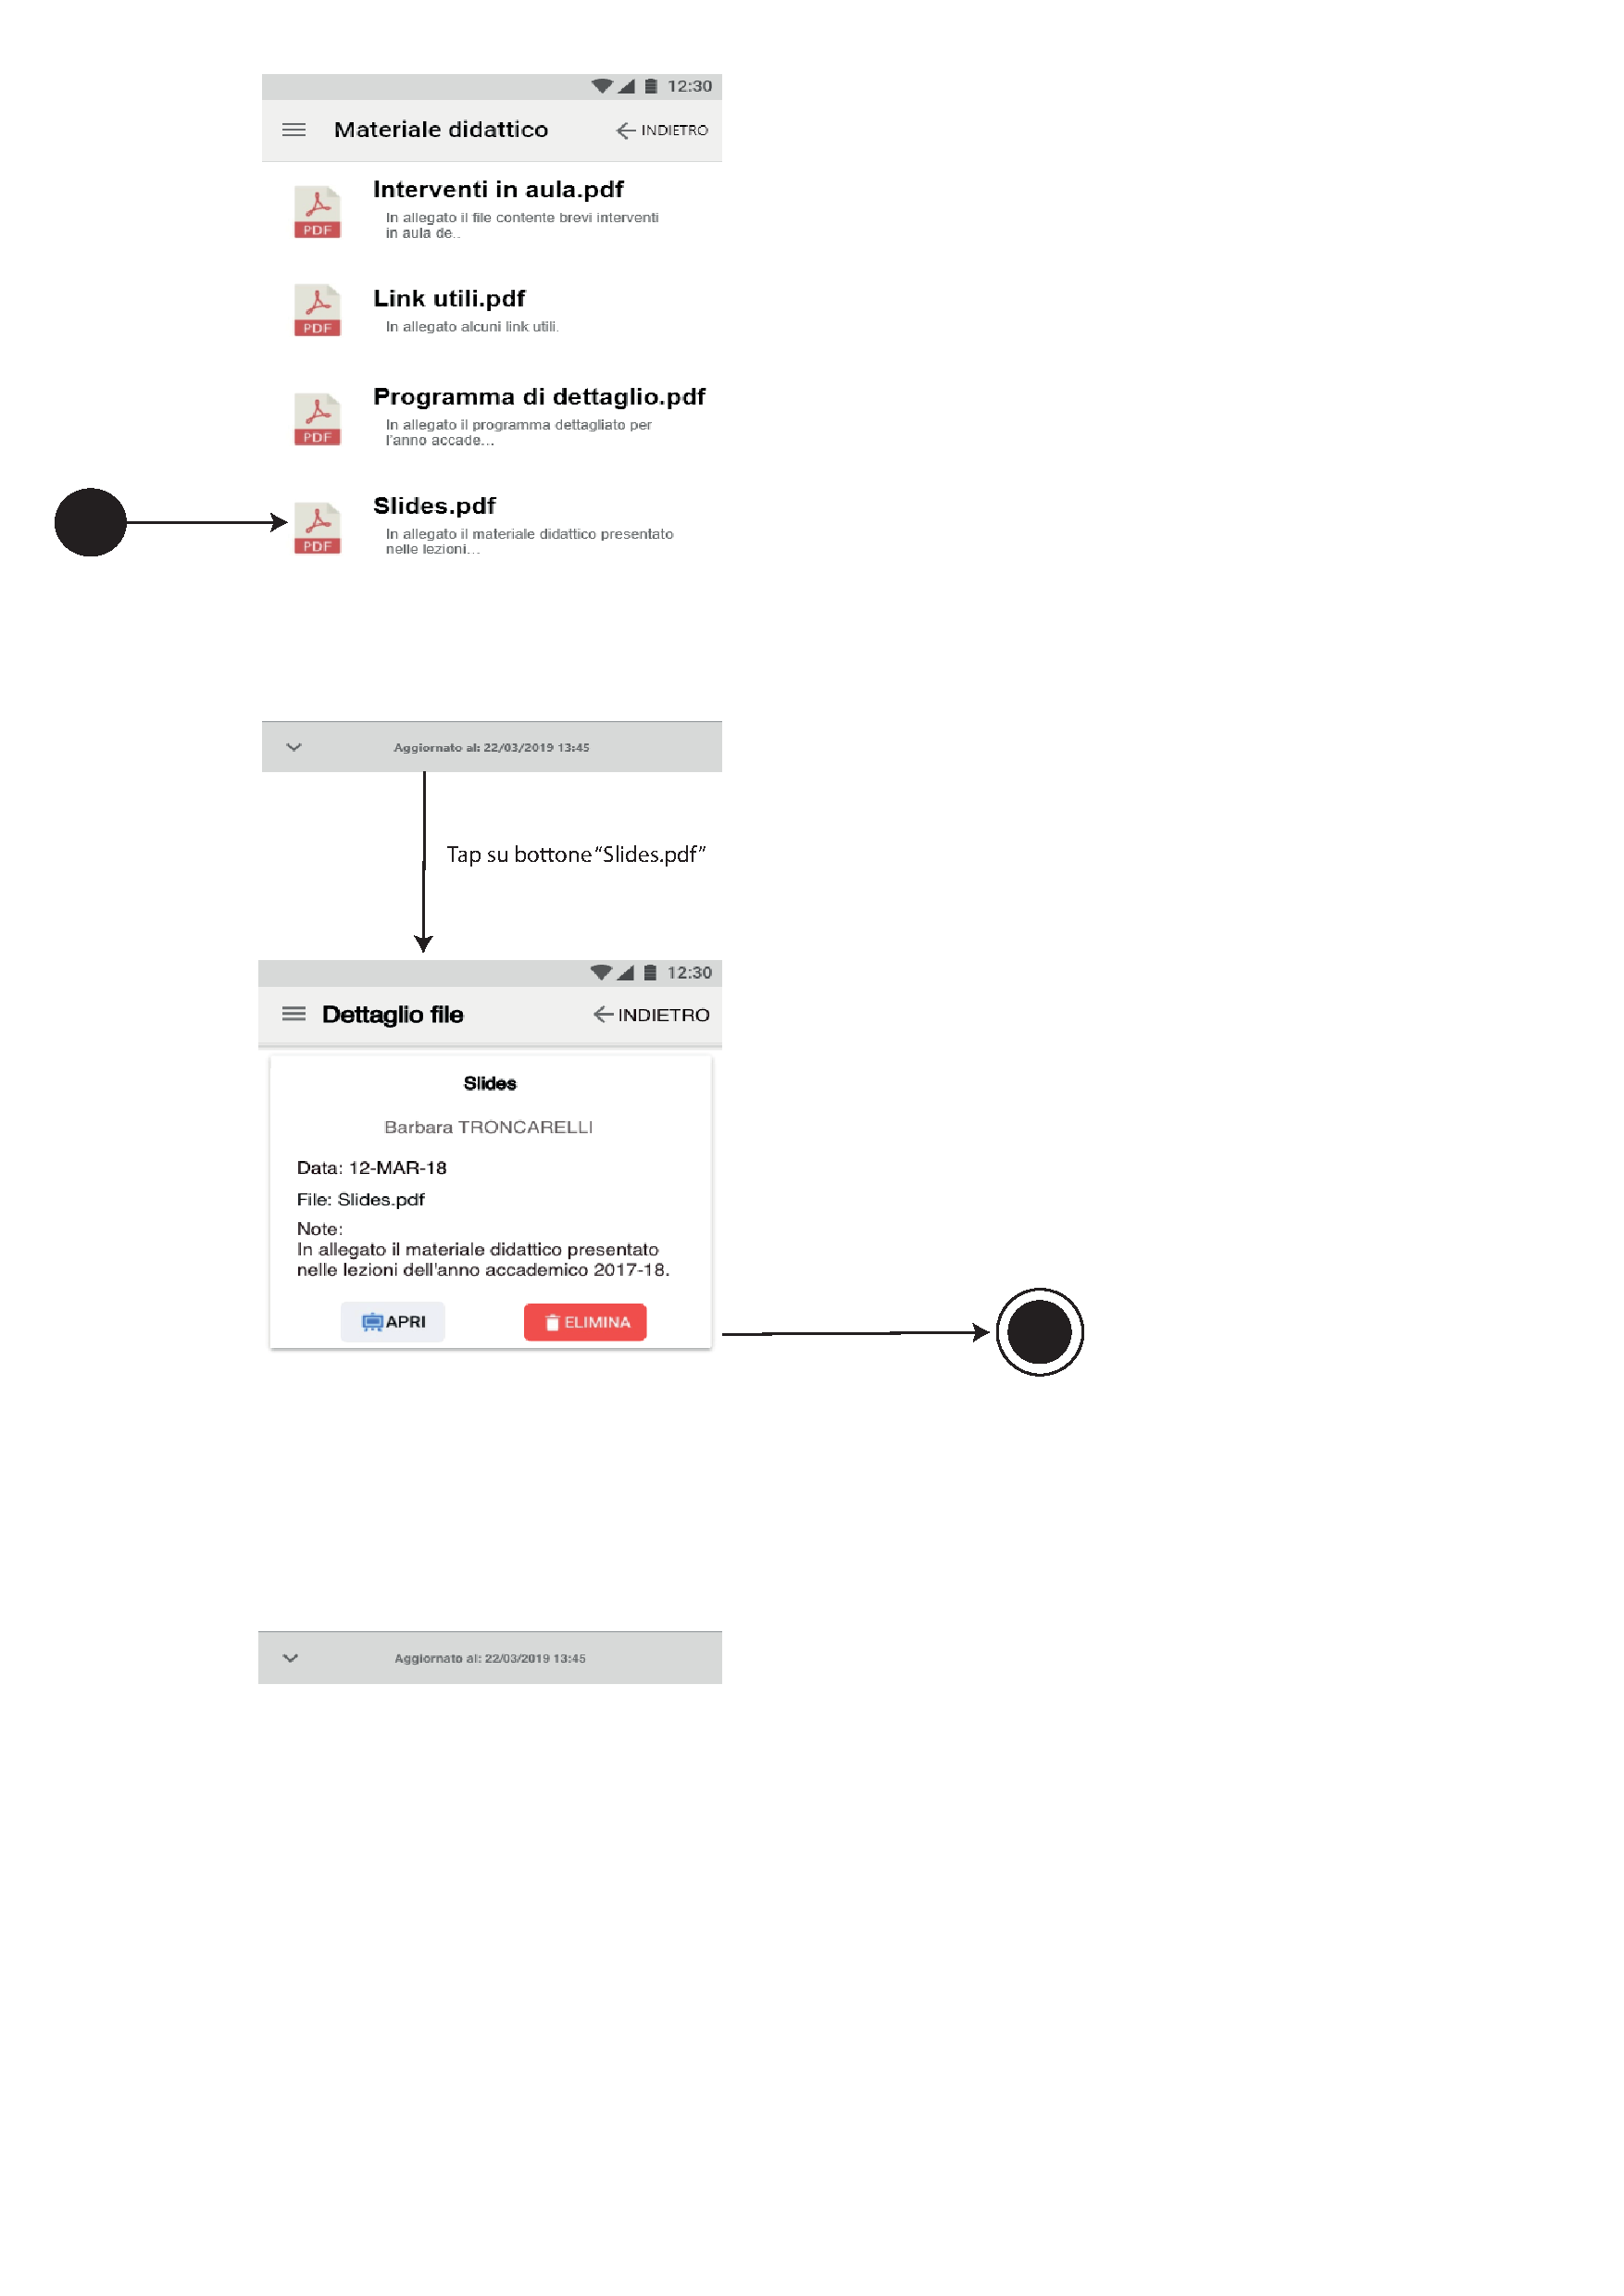
\includegraphics[width=6in]{imgs/gruppo1/activity_diagrams/AD15_dettagli_file.pdf}
\end{center}
\newpage

%%8.6.16 - Apri file%%

\subsection{Apri file}
\begin{center}
	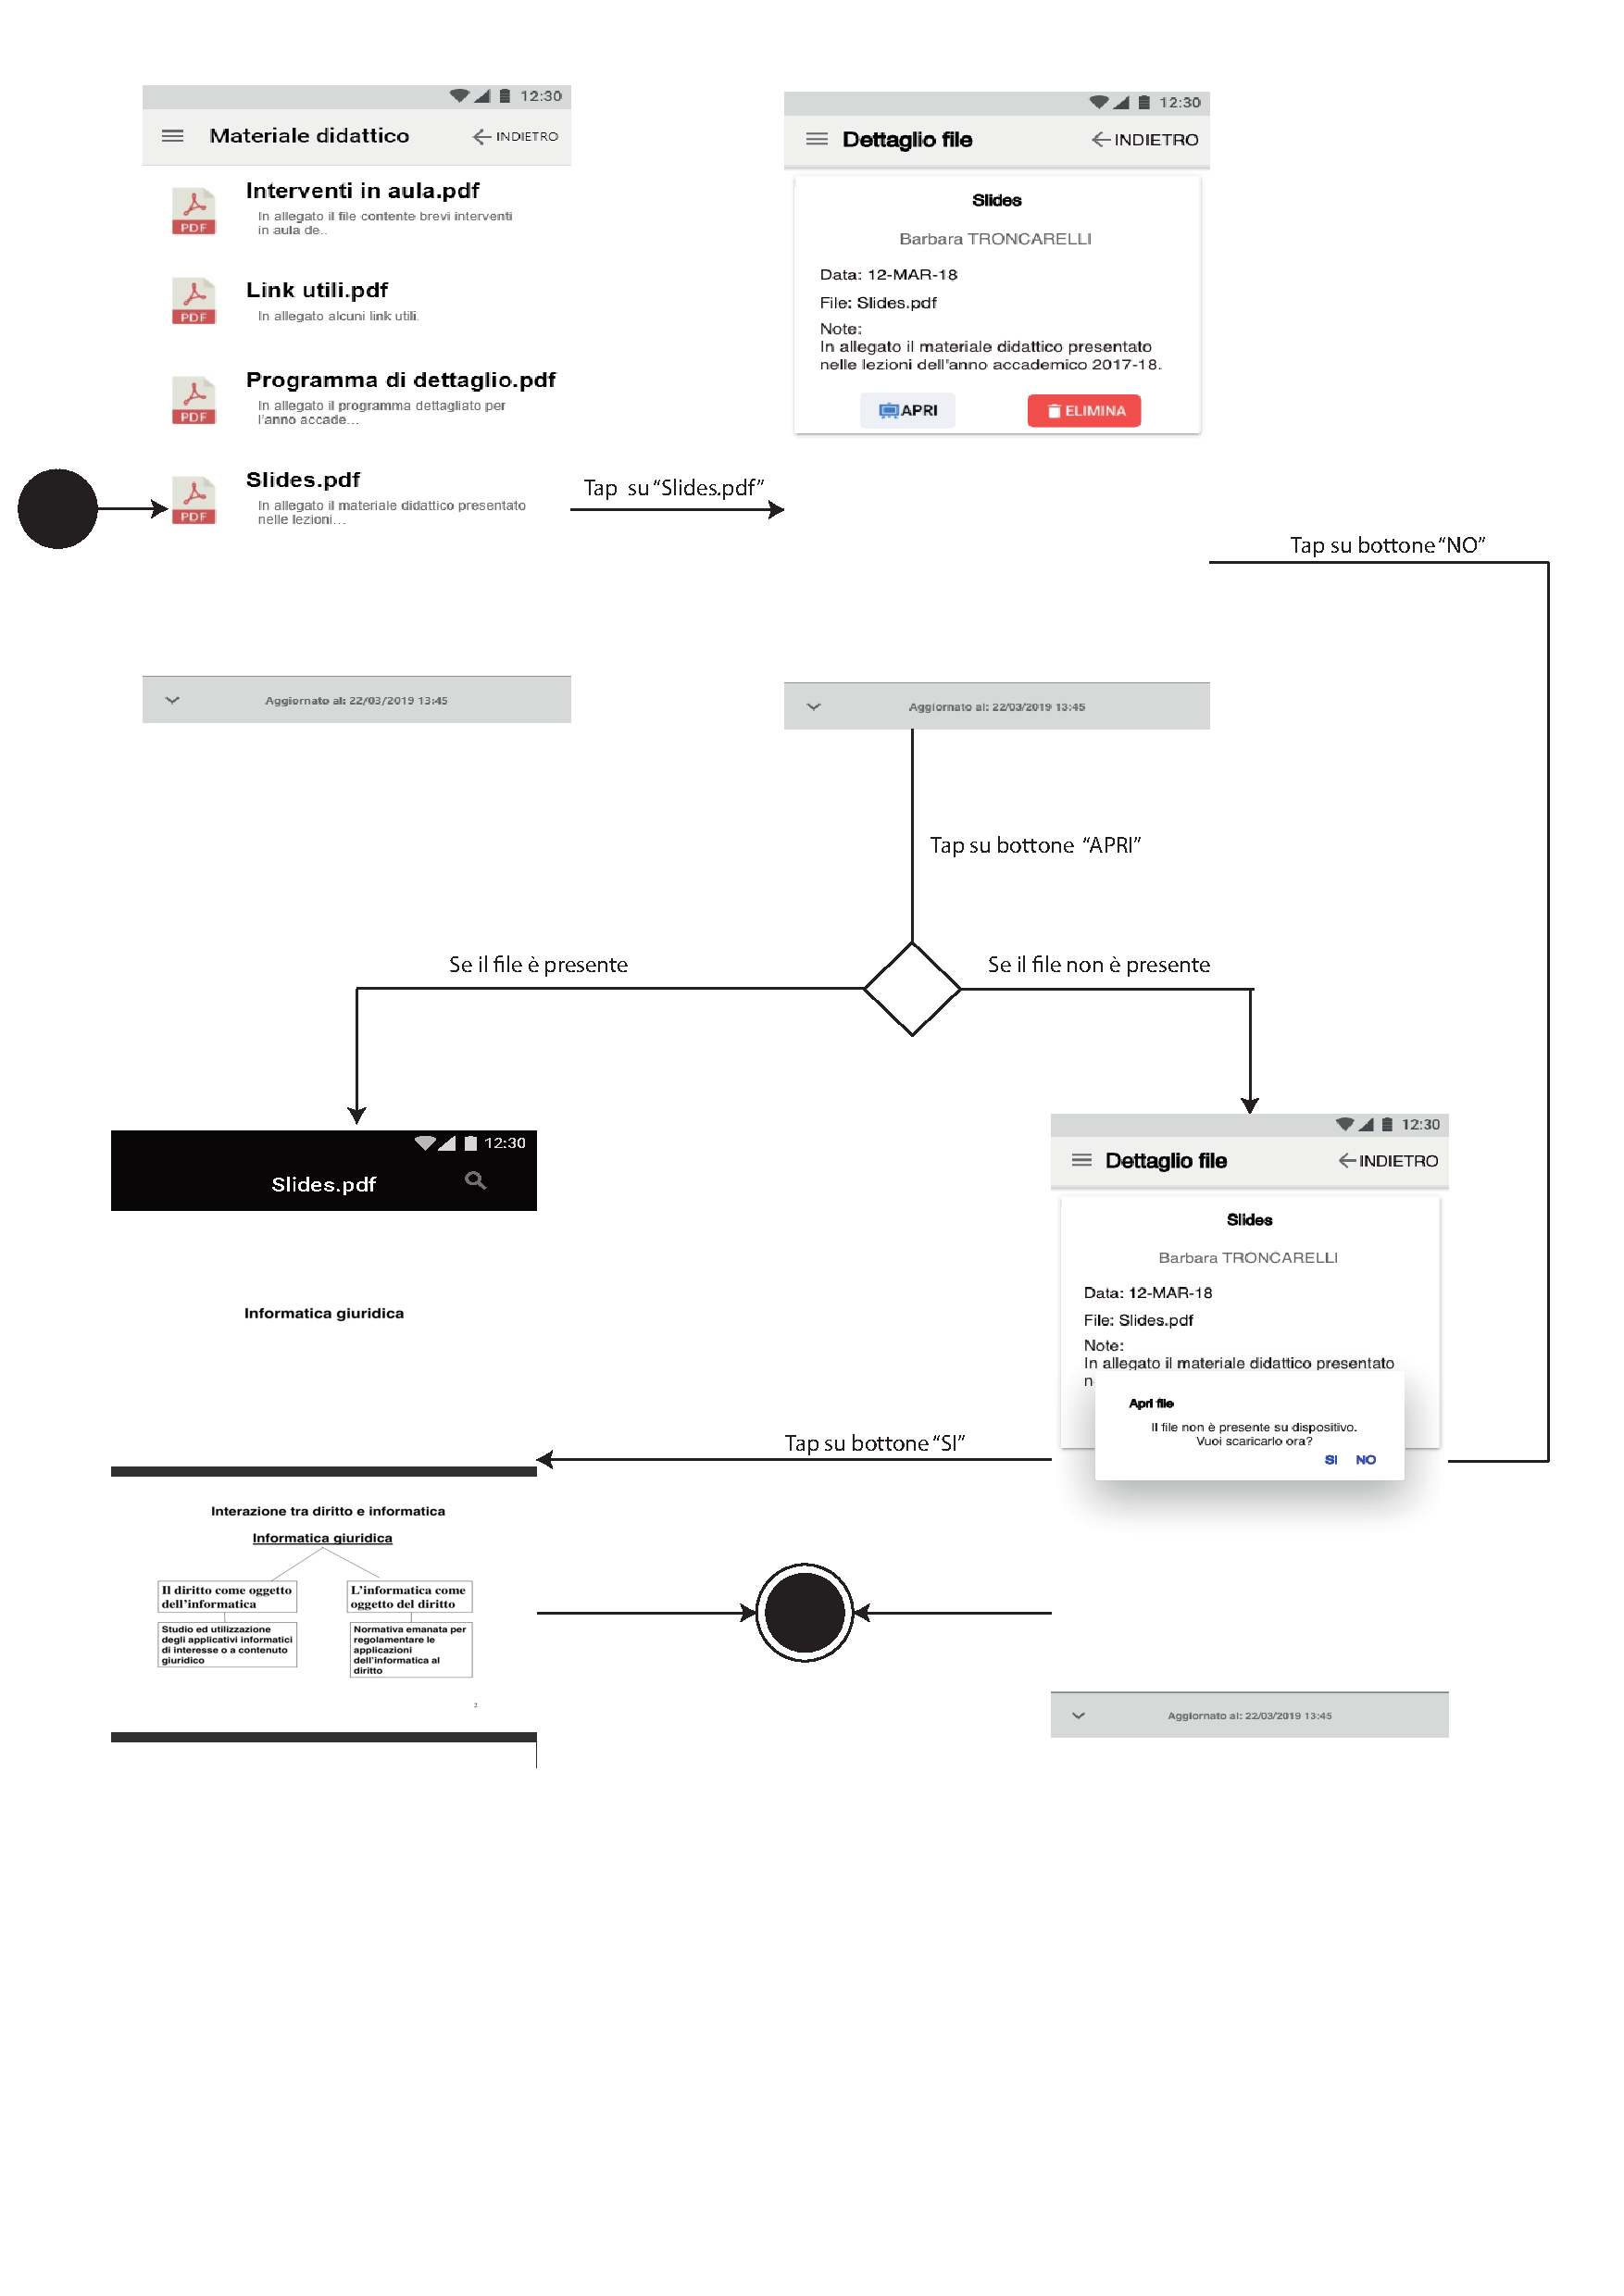
\includegraphics[width=6in]{imgs/gruppo1/activity_diagrams/AD16_apri_file.pdf}
\end{center}
\newpage

%%8.6.17 - Rimuovi file%%

\subsection{Rimuovi file}
\begin{center}
	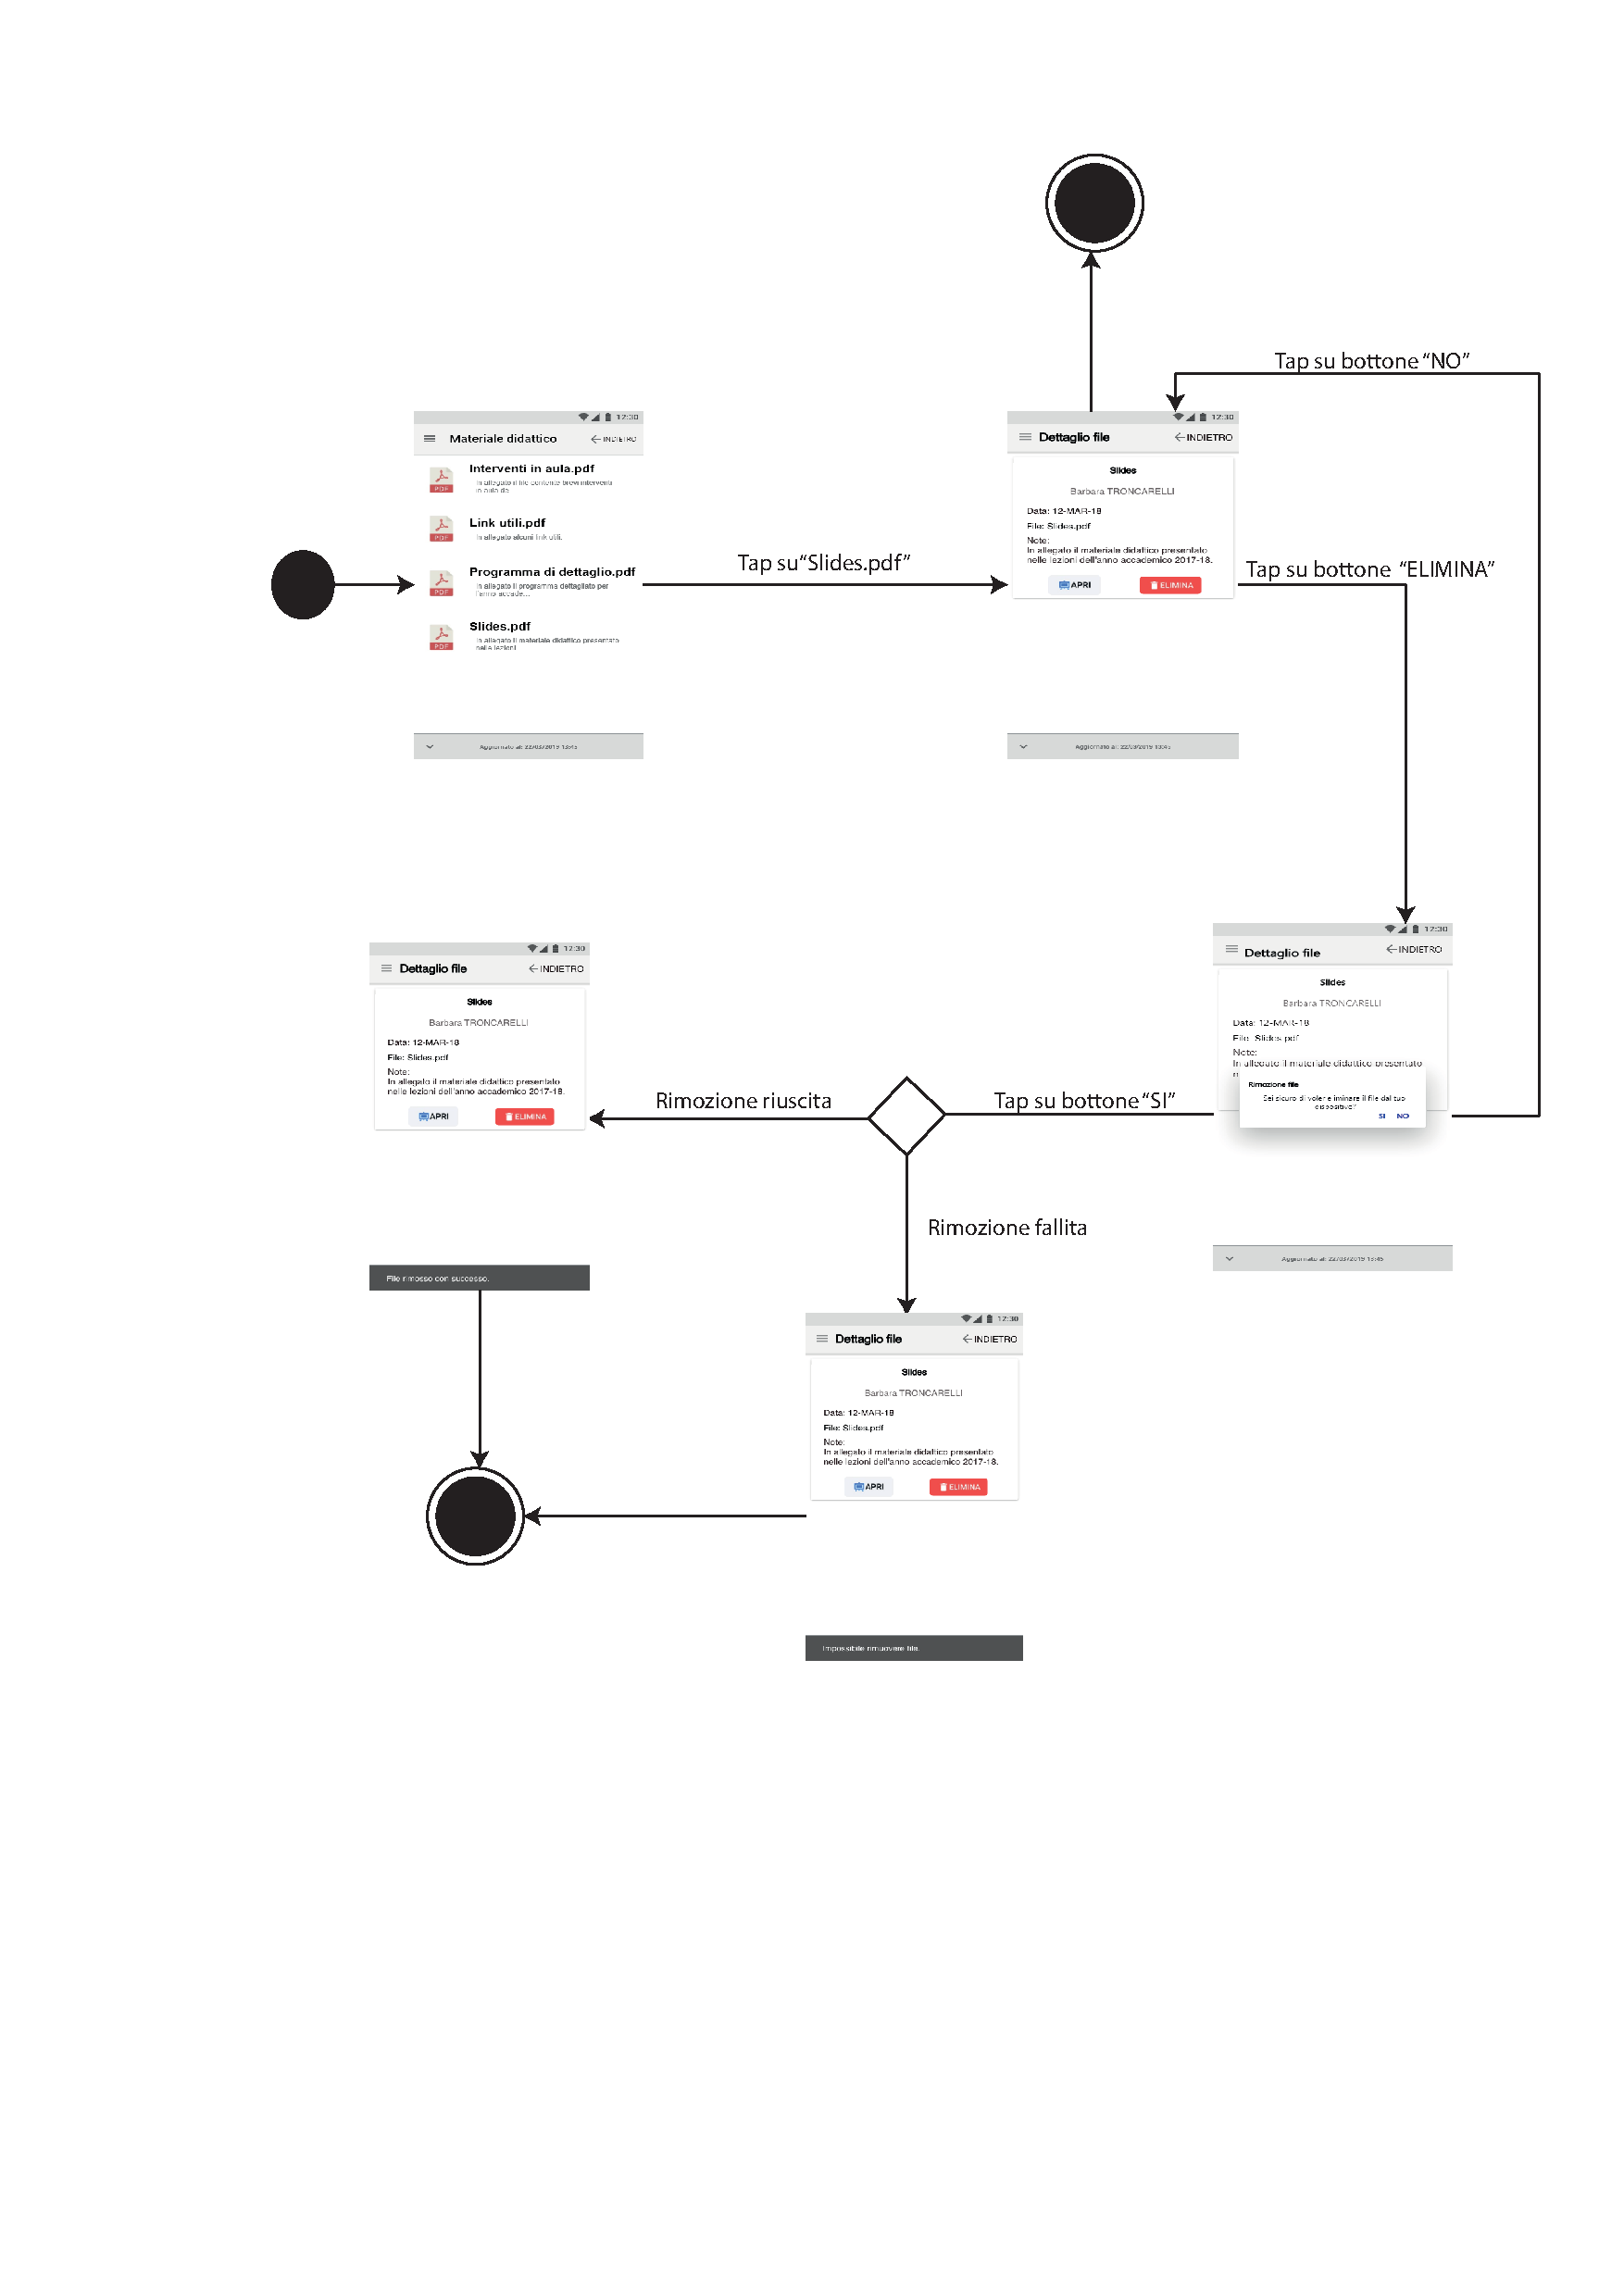
\includegraphics[width=6in]{imgs/gruppo1/activity_diagrams/AD17_rimuovi_file.pdf}
\end{center}
\newpage
